%%%%%%%%%%%%%%%%%%%%%%%%%%%%%%%%%%%%%%%%%
% Masters/Doctoral Thesis 
% LaTeX Template
% Version 2.5 (27/8/17)
%
% This template was downloaded from:
% http://www.LaTeXTemplates.com
%
% Version 2.x major modifications by:
% Vel (vel@latextemplates.com)
%
% This template is based on a template by:
% Steve Gunn (http://users.ecs.soton.ac.uk/srg/softwaretools/document/templates/)
% Sunil Patel (http://www.sunilpatel.co.uk/thesis-template/)
%
% Template license:
% CC BY-NC-SA 3.0 (http://creativecommons.org/licenses/by-nc-sa/3.0/)
%
%%%%%%%%%%%%%%%%%%%%%%%%%%%%%%%%%%%%%%%%%

%----------------------------------------------------------------------------------------
%	PACKAGES AND OTHER DOCUMENT CONFIGURATIONS
%----------------------------------------------------------------------------------------

\documentclass[
11pt, % The default document font size, options: 10pt, 11pt, 12pt
%oneside, % Two side (alternating margins) for binding by default, uncomment to switch to one side
english, % ngerman for German
singlespacing, % Single line spacing, alternatives: onehalfspacing or doublespacing
%draft, % Uncomment to enable draft mode (no pictures, no links, overfull hboxes indicated)
%nolistspacing, % If the document is onehalfspacing or doublespacing, uncomment this to set spacing in lists to single
%liststotoc, % Uncomment to add the list of figures/tables/etc to the table of contents
%toctotoc, % Uncomment to add the main table of contents to the table of contents
%parskip, % Uncomment to add space between paragraphs
%nohyperref, % Uncomment to not load the hyperref package
headsepline, % Uncomment to get a line under the header
%chapterinoneline, % Uncomment to place the chapter title next to the number on one line
%consistentlayout, % Uncomment to change the layout of the declaration, abstract and acknowledgements pages to match the default layout
]{MastersDoctoralThesis} % The class file specifying the document structure

\usepackage[utf8]{inputenc} % Required for inputting international characters
\usepackage[T1]{fontenc} % Output font encoding for international characters

\usepackage{mathpazo} % Use the Palatino font by default

%\usepackage[backend=biber,style=phys,natbib=true]{biblatex} % Use the bibtex backend with the authoryear citation style (which resembles APA)
%\usepackage[backend=biber,style=numeric,natbib=true]{biblatex} % Use the bibtex backend with the authoryear citation style (which resembles APA)
\usepackage[backend=biber,style=numeric-comp,natbib=true, sorting=none]{biblatex}
%\usepackage[backend=bibtex, style=phys]{biblatex}
%\usepackage[backend=bibtex, style=numeric]{biblatex}
%\usepackage[backend=bibtex, style=numeric, natbib=true]{biblatex}
%\usepackage[backend=bibtex, style=numeric-comp, natbib=true]{biblatex}

\addbibresource{LuizaCiucuMScThesisTrackML.bib} % The filename of the bibliography

\usepackage[autostyle=true]{csquotes} % Required to generate language-dependent quotes in the bibliography

\usepackage{tabularx}
\usepackage{adjustbox}
\usepackage{pdflscape}
\usepackage{multirow} % for tables
\usepackage{graphicx}
\usepackage{mathtools}

\def\ttbar{\ensuremath{t\bar{t}}}
\def\ttbaremu{\ensuremath{t\bar{t}~e-\mu}}
\def\pt{\ensuremath{p_{\mathrm{T}}}} % Subscript roman not italic (EE)

%
% +--------------------------------------------------------------------+
% |                                                                    |
% |  Some useful units                                                 |
% |                                                                    |
% +--------------------------------------------------------------------+
%
\def\TeV{\ifmmode {\mathrm{\ Te\kern -0.1em V}}\else
                   \textrm{Te\kern -0.1em V}\fi}%
\def\GeV{\ifmmode {\mathrm{\ Ge\kern -0.1em V}}\else
                   \textrm{Ge\kern -0.1em V}\fi}%
\def\MeV{\ifmmode {\mathrm{\ Me\kern -0.1em V}}\else
                   \textrm{Me\kern -0.1em V}\fi}%
\def\keV{\ifmmode {\mathrm{\ ke\kern -0.1em V}}\else
                   \textrm{ke\kern -0.1em V}\fi}%
\def\eV{\ifmmode  {\mathrm{\ e\kern -0.1em V}}\else
                   \textrm{e\kern -0.1em V}\fi}%
\let\tev=\TeV
\let\gev=\GeV
\let\mev=\MeV
\let\kev=\keV
\let\ev=\eV

\def\TeVc{\ifmmode {\mathrm{\ Te\kern -0.1em V}/c}\else
                   {\textrm{Te\kern -0.1em V}/$c$}\fi}%
\def\GeVc{\ifmmode {\mathrm{\ Ge\kern -0.1em V}/c}\else
                   {\textrm{Ge\kern -0.1em V}/$c$}\fi}%
\def\MeVc{\ifmmode {\mathrm{\ Me\kern -0.1em V}/c}\else
                   {\textrm{Me\kern -0.1em V}/$c$}\fi}%
\def\keVc{\ifmmode {\mathrm{\ ke\kern -0.1em V}/c}\else
                   {\textrm{ke\kern -0.1em V}/$c$}\fi}%
\def\eVc{\ifmmode  {\mathrm{\ e\kern -0.1em V}/c}\else
                   {\textrm{e\kern -0.1em V}/$c$}\fi}%
\let\tevc=\TeVc
\let\gevc=\GeVc
\let\mevc=\MeVc
\let\kevc=\keVc
\let\evc=\eVc

\def\TeVcc{\ifmmode {\mathrm{\ Te\kern -0.1em V}/c^2}\else
                   {\textrm{Te\kern -0.1em V}/$c^2$}\fi}%
\def\GeVcc{\ifmmode {\mathrm{\ Ge\kern -0.1em V}/c^2}\else
                   {\textrm{Ge\kern -0.1em V}/$c^2$}\fi}%
\def\MeVcc{\ifmmode {\mathrm{\ Me\kern -0.1em V}/c^2}\else
                   {\textrm{Me\kern -0.1em V}/$c^2$}\fi}%
\def\keVcc{\ifmmode {\mathrm{\ ke\kern -0.1em V}/c^2}\else
                   {\textrm{ke\kern -0.1em V}/$c^2$}\fi}%
\def\eVcc{\ifmmode  {\mathrm{\ e\kern -0.1em V}/c^2}\else
                   {\textrm{e\kern -0.1em V}/$c^2$}\fi}%
\let\tevcc=\TeVcc
\let\gevcc=\GeVcc
\let\mevcc=\MeVcc
\let\kevcc=\keVcc
\let\evcc=\eVcc

\def\mt{\ensuremath{m_{t}}}

%
% +--------------------------------------------------------------------+
% |                                                                    |
% |  Particles                       |
% |                                                                    |
% +--------------------------------------------------------------------+

\def\Zzero{\ensuremath{Z^{0}}}
\def\Zboson{\ensuremath{Z}}
\def\Wplus{\ensuremath{W^+}}
\def\Wminus{\ensuremath{W^-}}
\def\Wboson{\ensuremath{W}}%
\def\Wpm{\ensuremath{W^{\pm}}}%
\def\Wmp{\ensuremath{W^{\mp}}}%

%
% +--------------------------------------------------------------------+
% |                                                                    |
% |  NN, metrics                       |
% |                                                                    |
% +--------------------------------------------------------------------+

\def\volumeID{\texttt{\detokenize{volume_id}}}
\def\layerID{\texttt{\detokenize{layer_id}}}
\def\moduleID{\texttt{\detokenize{module_id}}}
\def\hitID{\texttt{\detokenize{hit_id}}}
\def\nbPositiveHit{\texttt{\detokenize{nbPositiveHit}}}
\def\nbTruePositiveHit{\texttt{\detokenize{nbTruePositiveHit}}}
\def\particleID{\texttt{\detokenize{particle_id}}}
%\def\\texttt{\detokenize{}}}
\def\nbBucket{\texttt{\detokenize{nbBucket}}}
\def\nbParticleTruth{\texttt{\detokenize{nbParticleTruth}}}
\def\nbParticleReco{\texttt{\detokenize{nbParticleReco}}}
\def\eff{\texttt{\detokenize{eff}}}

\def\TP{\ifmmode {\mathrm{TP}}\else
                   \textrm{TP}\fi}%
\def\FP{\ifmmode {\mathrm{FP}}\else
                   \textrm{FP}\fi}%                                     
\def\FN{\ifmmode {\mathrm{FN}}\else
                   \textrm{FN}\fi}%
\def\TN{\ifmmode {\mathrm{TN}}\else
                   \textrm{TN}\fi}%

\def\Accuracy{\ifmmode {\mathrm{Accuracy}}\else
                   \textrm{Accuracy}\fi}%
\def\Precision{\ifmmode {\mathrm{Precision}}\else
                   \textrm{Precision}\fi}%
\def\Recall{\ifmmode {\mathrm{Recall}}\else
                   \textrm{Recall}\fi}%
\def\NegativePredictedValue{\ifmmode {\mathrm{Negative~Predicted~Value}}\else
                   \textrm{Negative~Predicted~Value}\fi}%
\def\TrueNegativeRate{\ifmmode {\mathrm{True~Negative~Rate}}\else
                   \textrm{True~Negative~Rate}\fi}%
\def\LossFunctionHinge{\ifmmode {\mathrm{Loss~function~hinge}}\else
                   \textrm{Loss~function~hinge}\fi}%
\def\LossFunctionSquaredHinge{\ifmmode {\mathrm{Loss~function~squared~hinge}}\else
                   \textrm{Loss~function~squared~hinge}\fi}%
\def\ReLU{\ifmmode {\mathrm{ReLU}}\else
                   \textrm{ReLU}\fi}%
\def\ELU{\ifmmode {\mathrm{ELU}}\else
                   \textrm{ELU}\fi}%
\def\SQNL{\ifmmode {\mathrm{SQNL}}\else
                   \textrm{SQNL}\fi}%
\def\SOSI{\ifmmode {\mathrm{SOSI}}\else
                   \textrm{SOSI}\fi}%


\def\Ni{\ifmmode {\mathrm{N}_\mathrm{i}}\else
                   \textrm{N}_{\textrm{i}}\fi}%
\def\wi{\ifmmode {\mathrm{w}_\mathrm{i}}\else
                   \textrm{w}_{\textrm{i}}\fi}%
\def\xi{\ifmmode {\mathrm{x}_\mathrm{i}}\else
                   \textrm{x}_{\textrm{i}}\fi}%
\def\wzero{\ifmmode {\mathrm{w}_\mathrm{0}}\else
                   \textrm{w}_{\textrm{0}}\fi}%
\def\xzero{\ifmmode {\mathrm{x}_\mathrm{0}}\else
                   \textrm{x}_{\textrm{0}}\fi}%

%
% +--------------------------------------------------------------------+
% |                                                                    |
% |  Define input folder for our plots only once                       |
% |                                                                    |
% +--------------------------------------------------------------------+

\newcommand{\td}[1]{\texttt{\detokenize{#1}}}


%----------------------------------------------------------------------------------------
%	MARGIN SETTINGS
%----------------------------------------------------------------------------------------

\geometry{
	paper=a4paper, % Change to letterpaper for US letter
	inner=2.5cm, % Inner margin
	%outer=3.8cm, % Outer margin
	outer=2.5cm, % Outer margin
	bindingoffset=.5cm, % Binding offset
	top=1.5cm, % Top margin
	bottom=1.5cm, % Bottom margin
	%showframe, % Uncomment to show how the type block is set on the page
}

%----------------------------------------------------------------------------------------
%	THESIS INFORMATION
%----------------------------------------------------------------------------------------

\thesistitle{Track Reconstruction for a High-Luminosity LHC Detector using Deep Neural Networks} % Your thesis title, this is used in the title and abstract, print it elsewhere with \ttitle
\supervisor{Dr. Tobias \textsc{Golling}} % Your supervisor's name, this is used in the title page, print it elsewhere with \supname
\examiner{} % Your examiner's name, this is not currently used anywhere in the template, print it elsewhere with \examname
\degree{Master of Particle Physics} % Your degree name, this is used in the title page and abstract, print it elsewhere with \degreename
\author{Luiza Adelina \textsc{Ciucu}} % Your name, this is used in the title page and abstract, print it elsewhere with \authorname
\addresses{} % Your address, this is not currently used anywhere in the template, print it elsewhere with \addressname

\subject{Experimental Particle Physics} % Your subject area, this is not currently used anywhere in the template, print it elsewhere with \subjectname
\keywords{} % Keywords for your thesis, this is not currently used anywhere in the template, print it elsewhere with \keywordnames
\university{\href{https://www.unige.ch/}{University of Geneva}} % Your university's name and URL, this is used in the title page and abstract, print it elsewhere with \univname
\department{\href{https://www.unige.ch/sciences/en/larecherche/domainesderecherche/physique/}{Department of Physics}} % Your department's name and URL, this is used in the title page and abstract, print it elsewhere with \deptname
\group{\href{https://www.unige.ch/dpnc/en/groups/tobias-golling/home/}{Prof. Golling Research Group}} % Your research group's name and URL, this is used in the title page, print it elsewhere with \groupname
\faculty{\href{https://www.unige.ch/sciences/en/larecherche/domainesderecherche/physique/}{Faculty of Science}} % Your faculty's name and URL, this is used in the title page and abstract, print it elsewhere with \facname

\AtBeginDocument{
\hypersetup{pdftitle=\ttitle} % Set the PDF's title to your title
\hypersetup{pdfauthor=\authorname} % Set the PDF's author to your name
\hypersetup{pdfkeywords=\keywordnames} % Set the PDF's keywords to your keywords
}

\begin{document}

\frontmatter % Use roman page numbering style (i, ii, iii, iv...) for the pre-content pages

\pagestyle{plain} % Default to the plain heading style until the thesis style is called for the body content

%----------------------------------------------------------------------------------------
%	TITLE PAGE
%----------------------------------------------------------------------------------------

\begin{titlepage}
\begin{center}

\vspace*{.06\textheight}
{\scshape\LARGE \univname\par}\vspace{1.5cm} % University name
\textsc{\Large Master Thesis}\\[0.5cm] % Thesis type

\HRule \\[0.4cm] % Horizontal line
{\huge \bfseries \ttitle\par}\vspace{0.4cm} % Thesis title
\HRule \\[1.5cm] % Horizontal line
 
\begin{minipage}[t]{0.4\textwidth}
\begin{flushleft} \large
\emph{Author:}\\
\href{http://www.johnsmith.com}{\authorname} % Author name - remove the \href bracket to remove the link
\end{flushleft}
\end{minipage}
\begin{minipage}[t]{0.4\textwidth}
\begin{flushright} \large
\emph{Supervisor:} \\
\href{http://www.jamessmith.com}{\supname} % Supervisor name - remove the \href bracket to remove the link  
\end{flushright}
\end{minipage}\\[3cm]
 
\vfill

\large \textit{A thesis submitted in fulfilment of the requirements\\ for the degree of \degreename}\\[0.3cm] % University requirement text
\textit{in the}\\[0.4cm]
\groupname\\\deptname\\[2cm] % Research group name and department name
 
\vfill

{\large \today}\\[4cm] % Date
%\includegraphics{Logo} % University/department logo - uncomment to place it
 
\vfill
\end{center}
\end{titlepage}

%----------------------------------------------------------------------------------------
%	DECLARATION PAGE
%----------------------------------------------------------------------------------------

%\begin{declaration}
%\addchaptertocentry{\authorshipname} % Add the declaration to the table of contents
%\noindent I, \authorname, declare that this thesis titled, \enquote{\ttitle} and the work presented in it are my own. I confirm that:

%\begin{itemize} 
%\item This work was done wholly or mainly while in candidature for a research degree at this University.
%\item Where any part of this thesis has previously been submitted for a degree or any other qualification at this University or any other institution, this has been clearly stated.
%\item Where I have consulted the published work of others, this is always clearly attributed.
%\item Where I have quoted from the work of others, the source is always given. With the exception of such quotations, this thesis is entirely my own work.
%\item I have acknowledged all main sources of help.
%\item Where the thesis is based on work done by myself jointly with others, I have made clear exactly what was done by others and what I have contributed myself.\\
%\end{itemize}
 
%\noindent Signed:\\
%\rule[0.5em]{25em}{0.5pt} % This prints a line for the signature
 
%\noindent Date:\\
%\rule[0.5em]{25em}{0.5pt} % This prints a line to write the date
%\end{declaration}

%\cleardoublepage

%----------------------------------------------------------------------------------------
%	QUOTATION PAGE
%----------------------------------------------------------------------------------------

%\vspace*{0.2\textheight}

%\noindent\enquote{\itshape Thanks to my solid academic training, today I can write hundreds of words on virtually any topic without possessing a shred of information, which is how I got a good job in journalism.}\bigbreak

%\hfill Dave Barry

%----------------------------------------------------------------------------------------
%	ABSTRACT PAGE
%----------------------------------------------------------------------------------------

\begin{abstract}
\addchaptertocentry{\abstractname} % Add the abstract to the table of contents
%The Thesis Abstract is written here (and usually kept to just this page). The page is kept centered vertically so can expand into the blank space above the title too\ldots
In the context of the ATLAS detector upgrade for the Run-4, the number of collisions per bunch crossing (pile-up) is increased to about 200. The overlapping particle tracks make it very difficult to reconstruct all particle tracks. Alternative reconstruction methods become necessary. In this thesis a deep neural network  (DNN) is used on simulated data from LHC experiments. Tracks are reconstructed from groups of 20 particle hits in the detector, called buckets. The DNN input is the hit spatial coordinates x, y, z. In every bucket hits belonging to the particle with the largest number of hits in the bucket have an output label of 1, the rest an output label of -1. This situation corresponds to a machine learning multi-label problem, namely to predict for each hit in the bucket an output value of 1 or -1. The model hyper-parameters are optimised. Various models are compared with various figures of merit. Overall, an efficiency of particle reconstruction of 71.3\% is obtained.
\end{abstract}

%----------------------------------------------------------------------------------------
%	ACKNOWLEDGEMENTS
%----------------------------------------------------------------------------------------

\begin{acknowledgements}
\addchaptertocentry{\acknowledgementname} % Add the acknowledgements to the table of contents
%The acknowledgments and the people to thank go here, don't forget to include your project advisor\ldots
This project would not have been possible without the continuous support, encouragement and feedback of my supervisor Prof. Tobias Golling and my senior colleague and Ph.D. student Sabrina Amrouche. I would also like to express my gratitude to the ATLAS group of the University of Geneva for having welcomed me, including Prof. Giuseppe Iacobucci and Anna Sfyrla. I would also like to thank the professors from my lectures of the University of Geneva, who offered me a strong theoretical and practical foundation in particle physics. 

\end{acknowledgements}

%----------------------------------------------------------------------------------------
%	LIST OF CONTENTS/FIGURES/TABLES PAGES
%----------------------------------------------------------------------------------------

\tableofcontents % Prints the main table of contents

\listoffigures % Prints the list of figures

\listoftables % Prints the list of tables

%----------------------------------------------------------------------------------------
%	ABBREVIATIONS
%----------------------------------------------------------------------------------------

%\begin{abbreviations}{ll} % Include a list of abbreviations (a table of two columns)

%\textbf{LAH} & \textbf{L}ist \textbf{A}bbreviations \textbf{H}ere\\
%\textbf{WSF} & \textbf{W}hat (it) \textbf{S}tands \textbf{F}or\\

%\end{abbreviations}

%----------------------------------------------------------------------------------------
%	PHYSICAL CONSTANTS/OTHER DEFINITIONS
%----------------------------------------------------------------------------------------

%\begin{constants}{lr@{${}={}$}l} % The list of physical constants is a three column table

% The \SI{}{} command is provided by the siunitx package, see its documentation for instructions on how to use it

%Speed of Light & $c_{0}$ & \SI{2.99792458e8}{\meter\per\second} (exact)\\
%Constant Name & $Symbol$ & $Constant Value$ with units\\

%\end{constants}

%----------------------------------------------------------------------------------------
%	SYMBOLS
%----------------------------------------------------------------------------------------

%\begin{symbols}{lll} % Include a list of Symbols (a three column table)

%$a$ & distance & \si{\meter} \\
%$P$ & power & \si{\watt} (\si{\joule\per\second}) \\
%Symbol & Name & Unit \\

%\addlinespace % Gap to separate the Roman symbols from the Greek

%$\omega$ & angular frequency & \si{\radian} \\

%\end{symbols}

%----------------------------------------------------------------------------------------
%	DEDICATION
%----------------------------------------------------------------------------------------

%\dedicatory{For/Dedicated to/To my\ldots} 

%----------------------------------------------------------------------------------------
%	THESIS CONTENT - CHAPTERS
%----------------------------------------------------------------------------------------

\mainmatter % Begin numeric (1,2,3...) page numbering

\pagestyle{thesis} % Return the page headers back to the "thesis" style

% Include the chapters of the thesis as separate files from the Chapters folder
% Uncomment the lines as you write the chapters

\chapter{Introduction}
\label{chapter:Introduction}

Elementary particle physics is the field of physics that describes the elementary particles and their interactions. The theoretical model denoted by the Standard Model (SM) was created about 50 years ago and is a very successful theory. All its predictions have been confirmed experimentally, including the discovery of the Higgs boson in 2012 at CERN. But theorists believe that there are phenomena predicted by theories beyond the SM that may be discovered at CERN in the next decade, in the future data taking runs, Run-3 Run-4 and Run-5, at the Large Hadron Collider (LHC). There are four major experiments, two of which have general-purpose detectors: ATLAS and CMS. These experiments hope to discover new phenomena like supersymmetry and dark matter. These detectors are huge digital cameras in three dimensions (3D) made of three different layers. Inner detectors reconstruct tracks of charged particles and measure their momenta via ionization energy. Calorimeters measure the total energy of both charged and neutral particles in a destructive process. The final layer is the muon detector, which measures muons tracks as minimum ionization particles.

\ \\The LHC collides bunches of protons. The number of proton-pair collisions per bunch crossing (denoted by the pileup $\mu$) increases steadily every year, to maximise the probability to observe rare processes. Higher $\mu$ values indicate busier collision events and this makes it harder to reconstruct the particles. The latest value of $\mu$ in Run-2 ended in 2018 is about 36. In Run-4 a value of 200 is expected. The potential combinatorics of the events exceeds the available computing power, even with an increased budget. The solution is to reconstruct tracks via new machine learning techniques. This is the problem addressed in this thesis. A public simulated dataset for a general-purpose detector at $\mu$=200 produced for the TrackML Challenge is analyzed in this project. Two key techniques used are a deep neural network and an approximate nearest neighbour technique.

\ \\Sections~\ref{sec:StandardModel} and~\ref{sec:SMLimitations} describe the Standard Model and its limitations. Section~\ref{sec:ExperimentalSetup} describes the experimental setup, and Section~\ref{sec:ProtonCollisions} describes the proton collisions, and Section~\ref{sec:Tracking} describes the tracking reconstruction.

\section{Standard Model}
\label{sec:StandardModel}

The Standard Model is a theory that describes the elementary particle (fermions and bosons) and their interactions via three fundamental forces. The SM elementary particles are illustrated in Figure~\ref{fig:SMParticles} and are described in more detail below.

\begin{figure}[!htb]
  \centering
  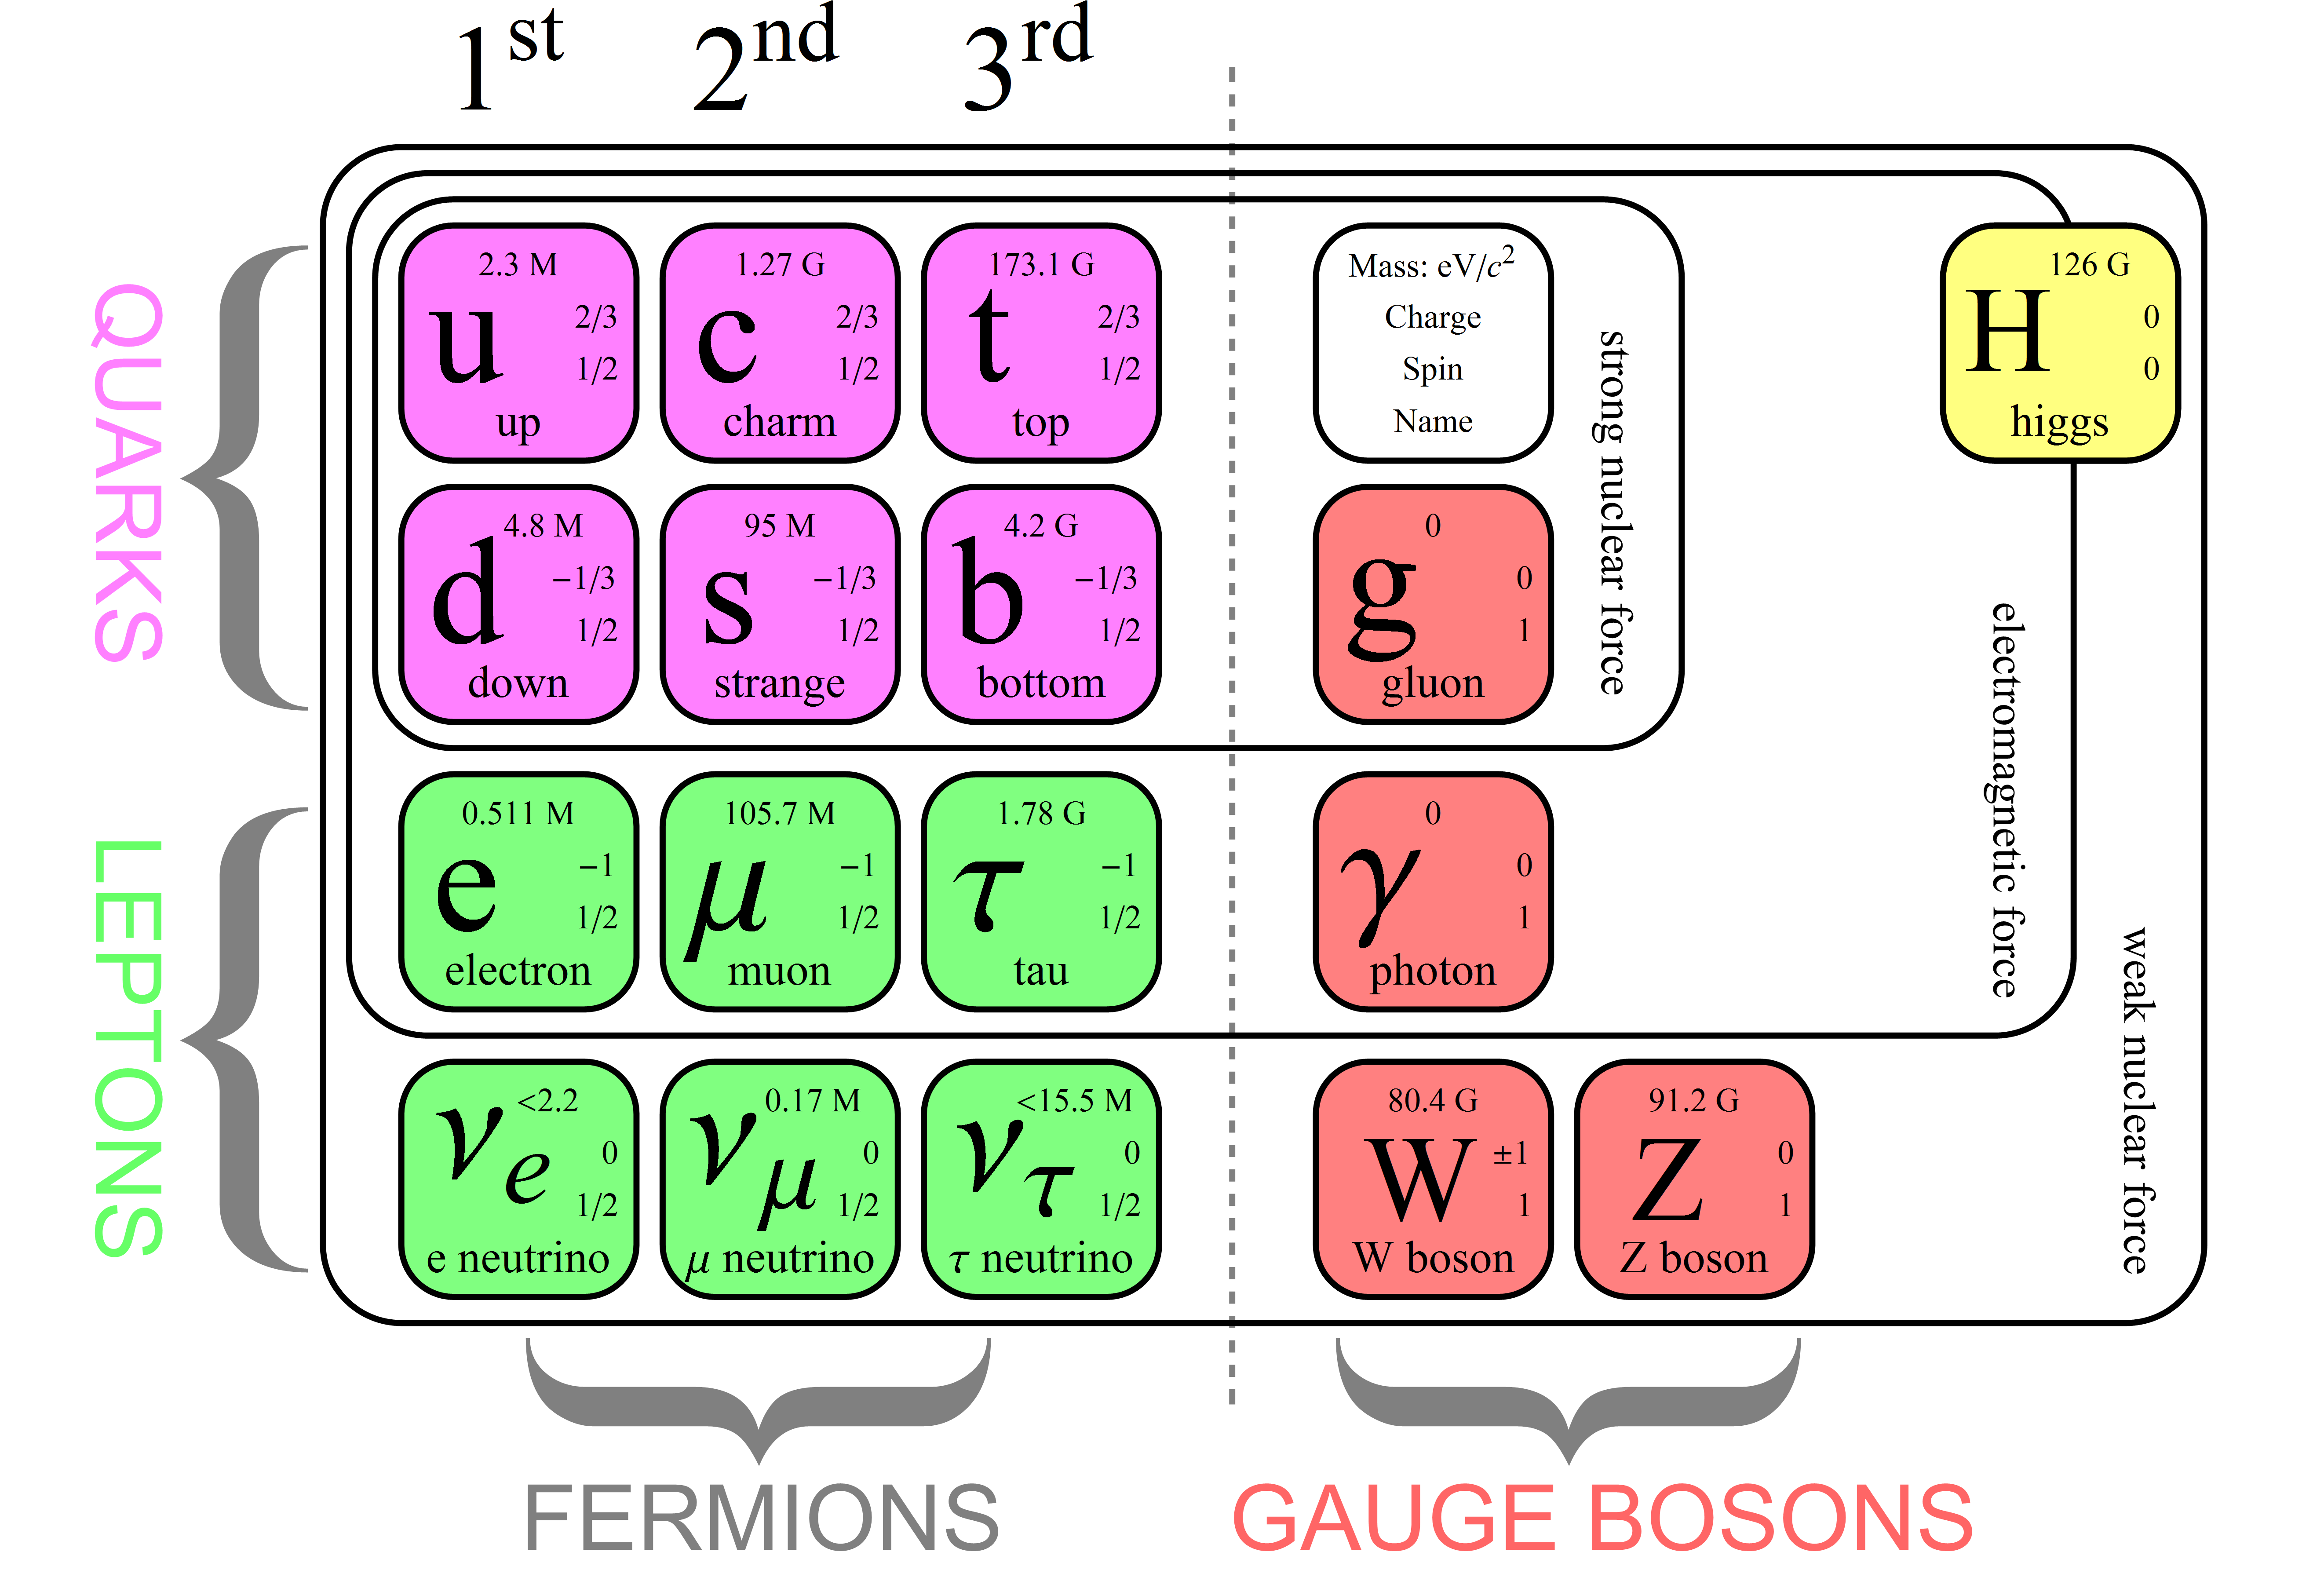
\includegraphics[width=0.98\textwidth]{./plots/SM.png}
  \caption{Elementary particles of the Standard Model}
  \label{fig:SMParticles}
\end{figure}

\ \\There are 12 fermions representing the constituents of matter. They have a semi-integer spin ($1/2$) and they are divided into two categories: quarks and leptons. The quarks have fractional electric charges and form baryons and mesons. The six quarks are up ($u\,^{+2/3}$), down ($d\,^{-1/3}$), charm ($c\,^{+2/3}$), strange ($s\,^{-1/3}$), top ($t\,^{+2/3}$), and bottom ($b\,^{-1/3}$). The three electrically-charged leptons have a negative charge: the electron ($e\,^{-}$), the muon ($\mu\,^{-}$), and the tau lepton ($\tau\,^{-}$). These have corresponding neutrally-charged leptons caled neutrinos ($\nu_e\,^0$, $\nu_\mu\,^0$, $\nu_\tau\,^0$). Together these particles form matter. For each matter particle there is an anti-matter particle that has an opposite electric charge. 

\ \\Fermions interact with each other via the exchange of elementary particles called bosons. Bosons are carriers of the elementary forces and have integer spin ($1$). There are eight type of gluons ($g$) that carry the strong force. The photon ($\gamma$) is responsible for the electromagnetic force. The \Wplus, \Wminus~and the \Zzero~bosons carry the weak force. 

\ \\There is also another type of boson, a scalar elementary particle of spin zero (0), called the Higgs boson. The Higgs boson is the latest elementary particle of the Standard Model discovered in 2012, by the ATLAS and CMS collaborations at CERN. It is predicted by the mechanism explaining how the elementary particles acquire mass.

\section{Limitations of the Standard Model}
\label{sec:SMLimitations}

Although all particles predicted by the Standard Model have been discovered, there are phenomena not yet explained by the SM. 

\ \\The matter-antimatter asymmetry is not yet understood. It is believed in the Big Bang equal quantities of matter and antimatter were produced. But the observable Universe seems to consist of matter only.

\ \\The matter-energy content of the Universe consists of only 5\% of regular baryonic matter. About 25\% is represented by dark matter, an unknown form of matter that interacts only very weakly with regular matter. It is thought this matter is key to the evolution of the Universe.

%\ \\The unification of known fundamental forces is not yet complete. The Standard Model is made of two theories put side by side: the electroweak theory and the quantum chromodynamics, which explains the strong interaction. But these two forces have not yet been unified. Such a unification is thought to happen at energies much larger than those available at the LHC. Such a theory would be called the Grand Unified Theory (GUT). If such a theory were combined further with the gravitational theory at energies close to the Big Bang, the theory of everything (TOE) would emerge.

%\ \\There are three generations of elementary particles. It is not clear why there are exactly three. Particles of each generation are more massive than the previous, but the exact mass values are not yet predicted from first principles. The Higgs mechanism explains how a particle can acquire mass by interacting with the Higgs boson proportional to its mass, but does not predict what the mass is. 

\ \\Overall, it is believed that the Standard Model is in fact only a low-energy approximation of a higher-energy theory. New particles and interactions are predicted by a variety of models of physics beyond the Standard Model (BSM). Such models have already been ruled out by current searches at CERN. The search for new physics will continue in Run-3, Run-4 and Run-5 at the LHC.

\section{Experimental Setup}
\label{sec:ExperimentalSetup}

At the moment the Large Hadron Collider (LHC), which is situated at CERN, is the most powerful proton-proton collider in the world. After the Tevatron and the Large Electron-Positron Collider (LEP) era, a new machine was needed for new discoveries in particle physics. The LHC was designed to achieve a centre-of-mass energy $\sqrt{s}=14\,\TeV$. Two of the biggest goals of the LHC are to study and test the SM, as well as to search for new physics BSM. The LHC accelerator complex is illustrated in Figure~\ref{fig:LHC}.

\begin{figure}[!htb]
  \centering
  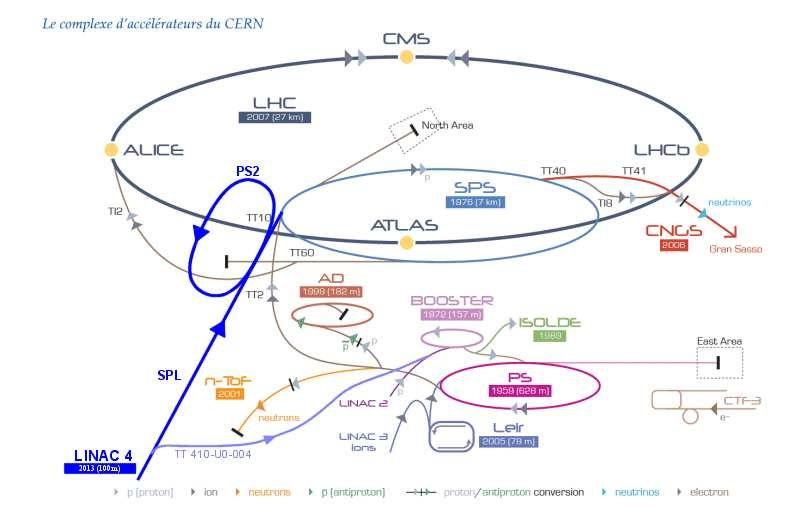
\includegraphics[width=0.5\textwidth]{plots/LHC.png} 
  \caption{LHC Accelerator Complex}
  \label{fig:LHC}
\end{figure}

\ \\This project is affiliated to the international collaboration of the A Toroidal LHC ApparatuS (ATLAS)~\cite{ATLAS}\cite{ATLASUrl}. ATLAS is the largest of several detectors at the LHC. ATLAS is one of two general-purpose particle physics detectors at the LHC, the other being CMS. The two collaborations of ATLAS and CMS perform similar research programs. New discoveries must be observed by both detectors to be believed as true. 

\ \\ATLAS is a cylindrical detector around the colliding proton beams. It is formed of four main subdetectors. The closest to the beam is the inner detector (ID). The ID measures the momentum vector of charged particles which ionise the gas inside the detector. An electric current is measured, giving the position of the particle in the detector, also called a \emph{hit}. A collection of hits forms a \emph{track}. The next detectors the particle encounters are two types of calorimeters, which measure the energy of the particle in a destructive way. The calorimeter is formed of two parts. First there is the electromagnetic calorimeter (EMCal), which measures the energy of electrons, positrons and photons. Then the hadronic calorimeter (HadCal), which measures the energy of hadrons, which originate from quarks and gluons. Several hadrons travelling together, after having originated in the same particle, are called \emph{jets}. Muons deposit very little energy in the calorimeters, being minimum ionising particles. The fourth subdetector detects energy depositions of muons and thus measures their momenta. These subdetectors of ATLAS are illustrated in Figure~\ref{fig:ATLAS}.

\begin{figure}[!htb]
  \centering
  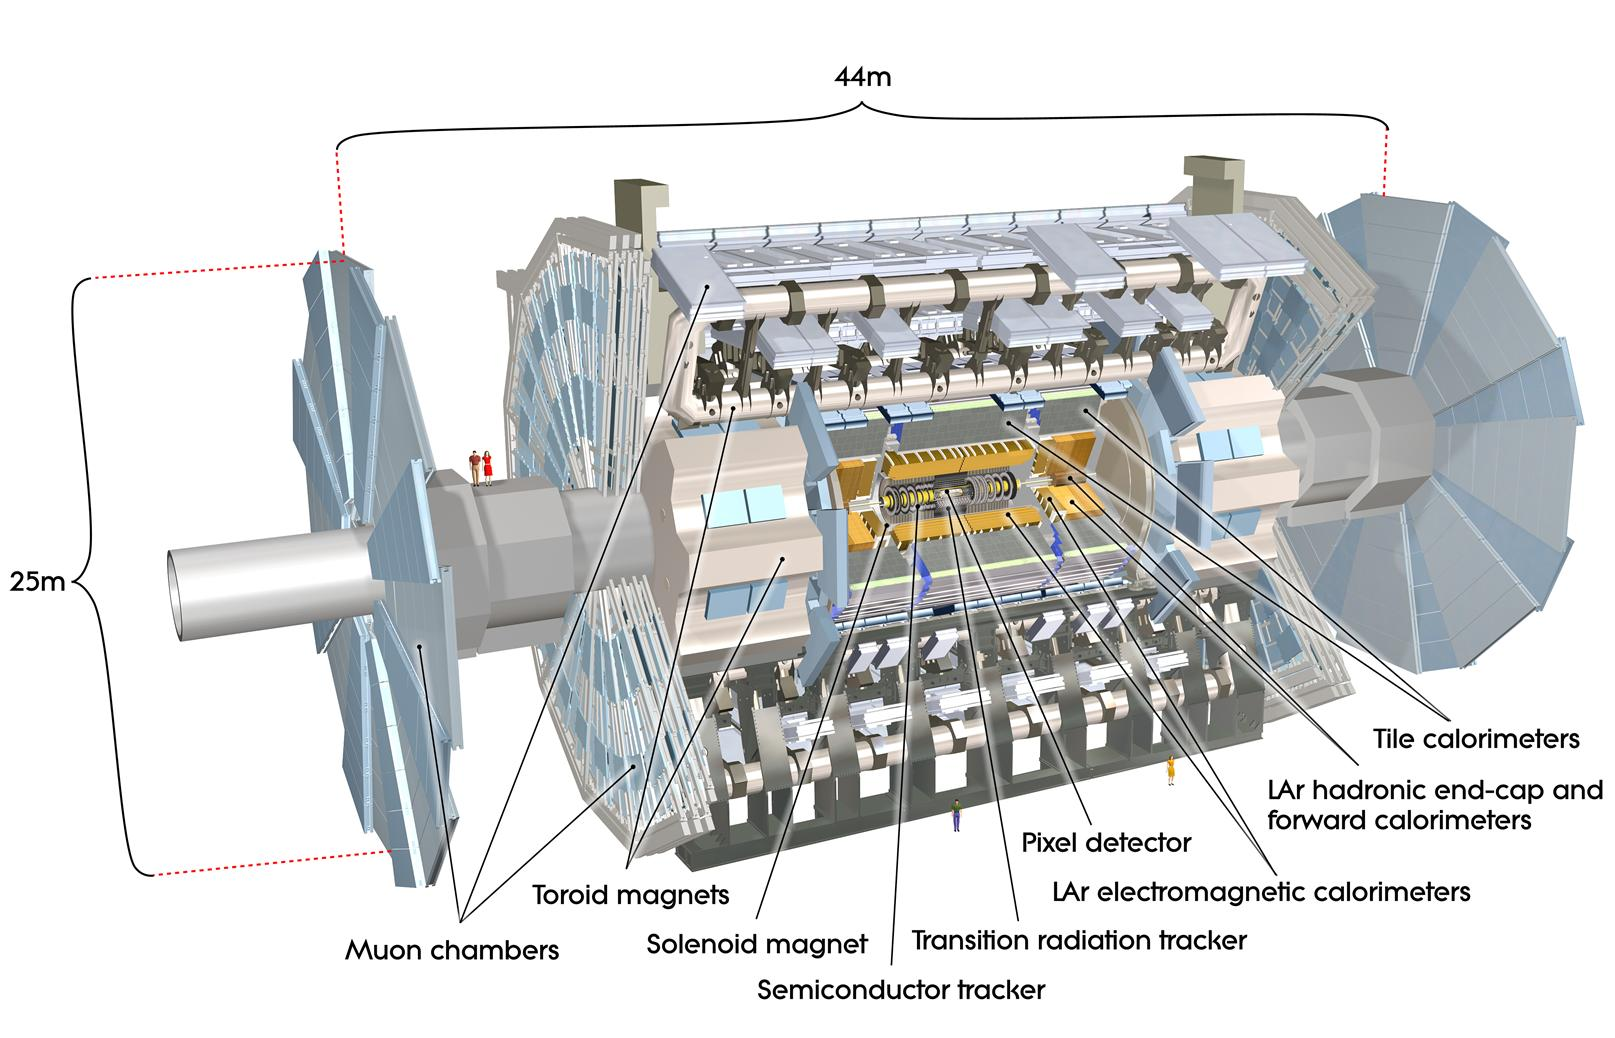
\includegraphics[width=0.5\textwidth]{plots/ATLAS.jpg} 
  \caption{ATLAS detector and its sub-detectors}
  \label{fig:ATLAS}
\end{figure}

\section{Proton Collisions}
\label{sec:ProtonCollisions}

The LHC collides proton beams head-on. The beam is not continuous. Instead, the protons are grouped into up to 2808 bunches. Each bunch contains approximately 115 billion protons. Proton bunches collide every 25 nanoseconds (ns), at a bunch collision rate of 40 MHz. The number of proton collisions during a bunch crossing is called \emph{pile-up} and is denoted by $\mu$. The data from the proton collisions from one bunch crossing are recorded together by the detector, called an an \emph{event}. Usually only one of the collisions produces a rare interesting particle, such as a top quark, a W, Z, or Higgs boson, or BSM particles like supersymmetric candidates or dark matter. The remaining collisions represent a background for the rare one. The rare collision is called \emph{hard scatter} (HS) and the rest of the collisions are called \emph{pile-up} collisions (PU). Event reconstruction in general and charged-particle track reconstruction in particular becomes \emph{harder} with increasing $\mu$. 

\ \\Yet increasing $\mu$ is exactly the strategy employed at the LHC for Run-1 and Run-2, in order to increase the collision luminosity and thus the probability to produce rare particles. The $\mu$ average values during Run-2 were about 13, 25, 38, 36 in 2015, 2016, 2017 and 2018, respectively, as seen in Figure~\ref{fig:LHCPileup}~\cite{ATLASPileup}. In Run-3, Run-4 and Run-5, the aim is to increase the pile-up even further to $\mu=200$.

\begin{figure}[!htb]
  \centering
  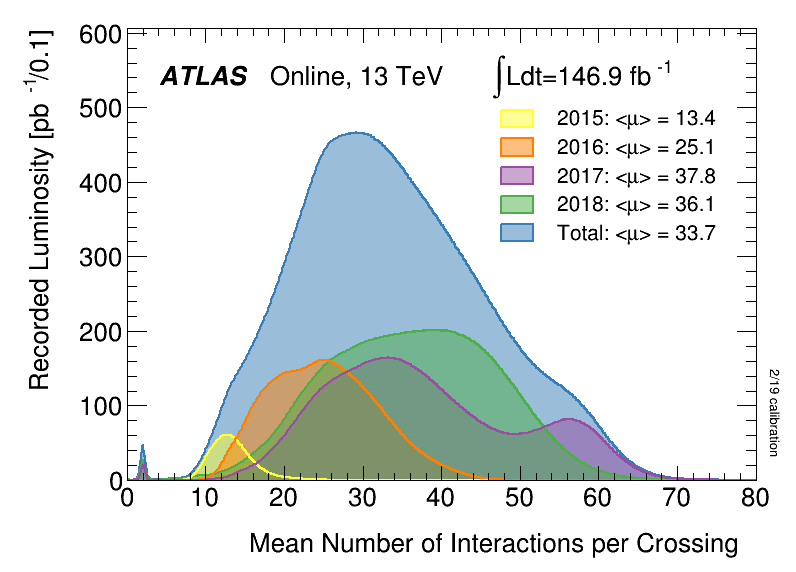
\includegraphics[width=0.5\textwidth]{plots/ATLAS_mu_2015_2018.png} 
  \caption{LHC pile-up ($\mu$) increase during Run-2~\cite{ATLASPileup}}
  \label{fig:LHCPileup}
\end{figure}

\section{Tracking}
\label{sec:Tracking}

A group of hits reconstructed in the inner detector (ID) and belonging to the same particle is called a \emph{track}. Reconstructing particle tracks is called \emph{tracking}. Tracks are produced only by charged particles that ionise the gas in the ID. The ID is held in a magnetic field, so that the trajectories of positively and negatively charged particles curve in opposite directions. The radius of the curvature allows measurement of the particle momentum. Neutral particles, such as photons, neutrinos, and neutral hadrons, do not produce tracks. Because of the magnetic field, tracks are geometric helices pointing approximately to the origin of the primary proton-proton interaction. Reconstructing one track from hits is illustrated in Figure~\ref{fig:FromHitsToTracks}. Reconstructed hits and tracks for an entire collision event are overlaid in Figure~\ref{fig:FromHitsToTracks2}, using simulated data for a general-purpose particle detector. The data is from the TrackML Challenge dataset used in this project. 

\begin{figure}[!htb]
\centering
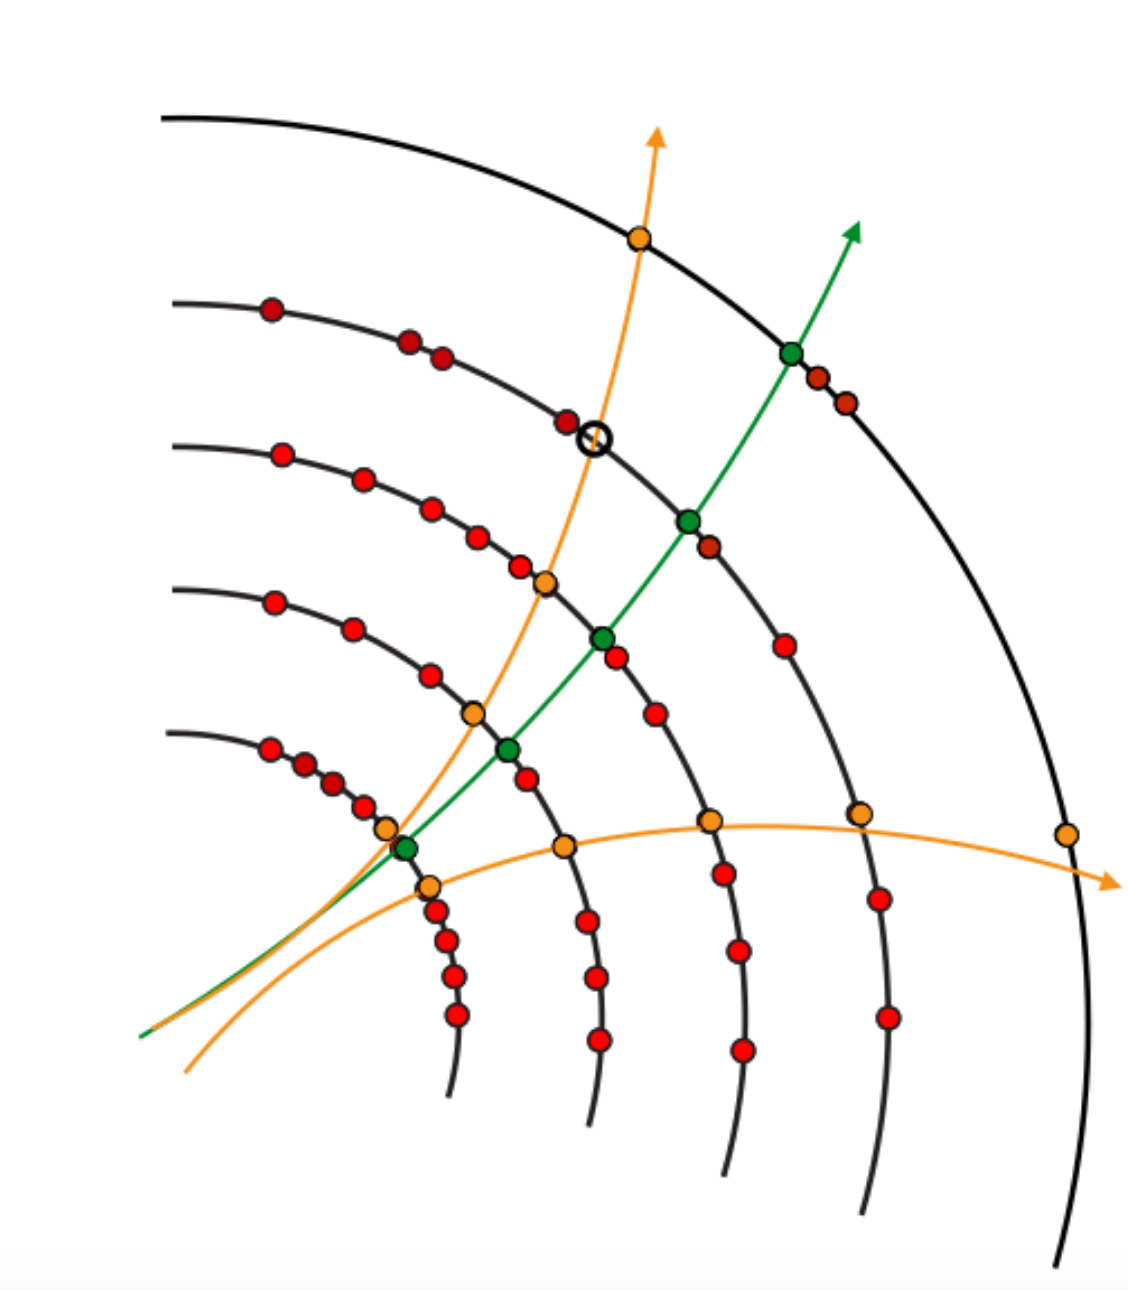
\includegraphics[width=0.30\textwidth]{./plots/TrackReconstruction.png}
\caption{Reconstructing one track from hits in a general-purpose detector. In green a good reconstruction, in orange two bad reconstructions~\cite{TrackMLPPTBefore}.}
\label{fig:FromHitsToTracks}
\end{figure}

\begin{figure}[!htb]
\centering
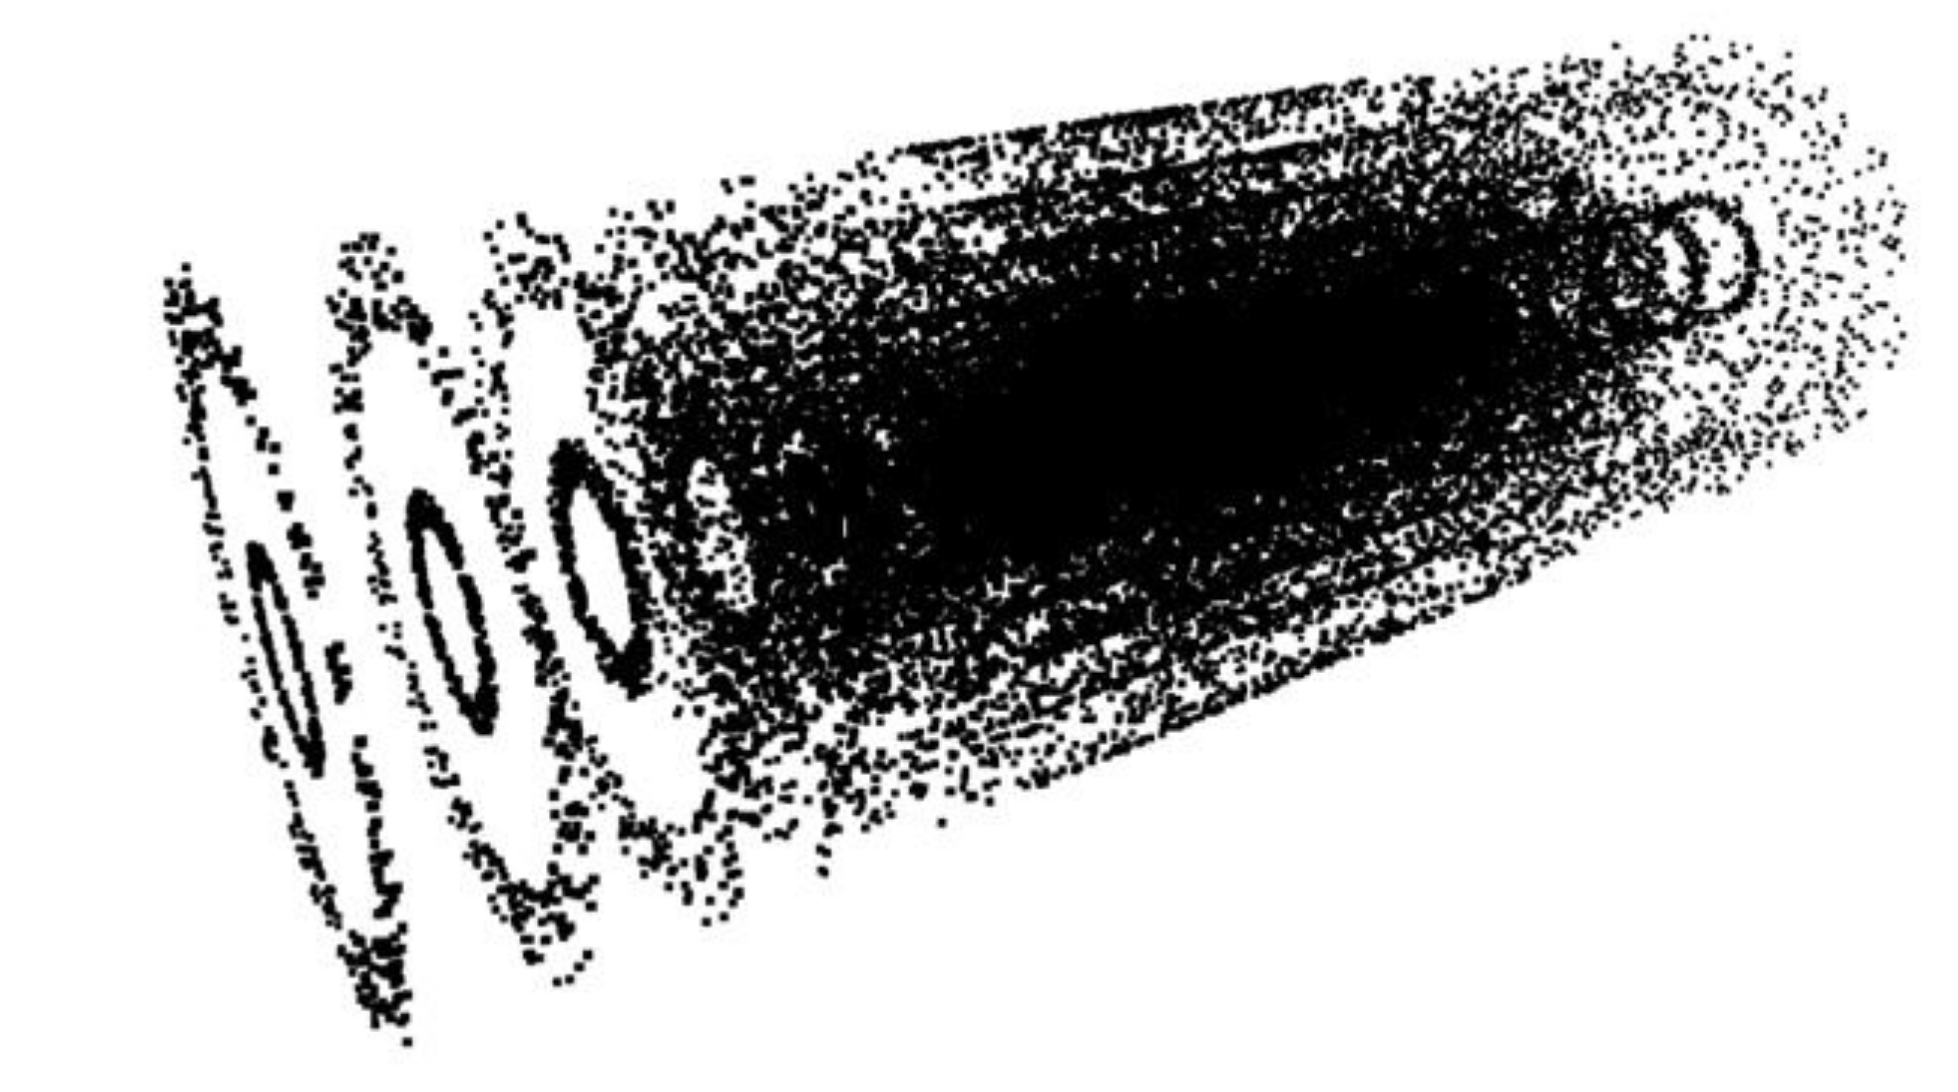
\includegraphics[width=0.49\textwidth]{./plots/Hits.png}
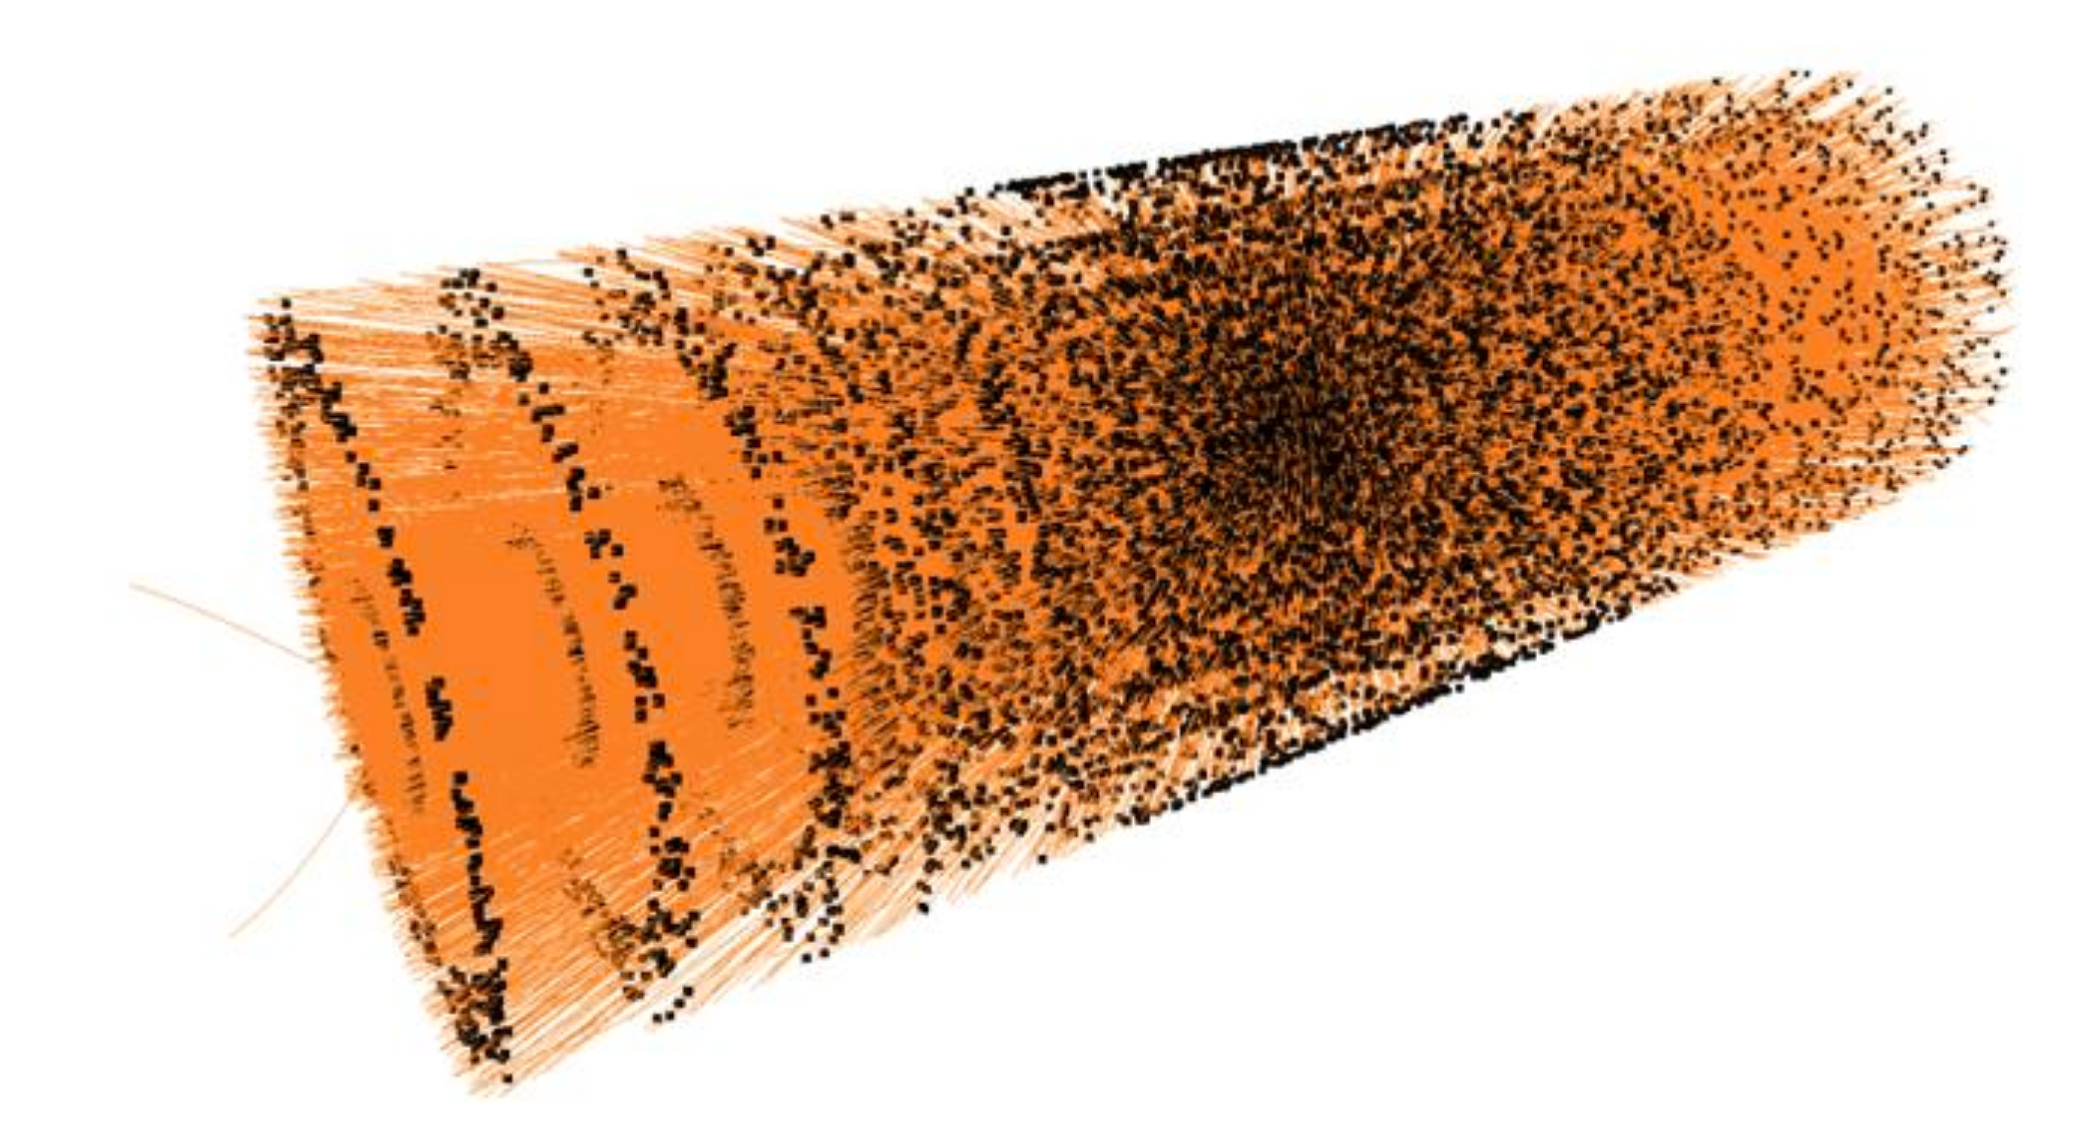
\includegraphics[width=0.49\textwidth]{./plots/Tracks.png}
\caption{Tracking for a general-purpose detector illustrated by reconstructing tracks (orange lines to the right) from hits (black individual 3D points to the left)~\cite{TrackMLPPTAfter}~\cite{TrackMLPPTAfter2}.}
\label{fig:FromHitsToTracks2}
\end{figure}

\ \\Tracking is a key component of event reconstruction and is used in several of its steps. The first step is to reconstruct vertices. Every proton collision in a bunch-crossing produces its own particles, out of which only the charged particles produce tracks. These tracks are clustered in a vertex. From the vertices in an event, the most interesting one (usually at higher energy for a rare particle) is called the \emph{primary vertex}, the rest being \emph{pile-up vertices}, as illustrated in Figure~\ref{fig:Vertices} for the ATLAS detector. 

\begin{figure}[!htb]
  \centering
  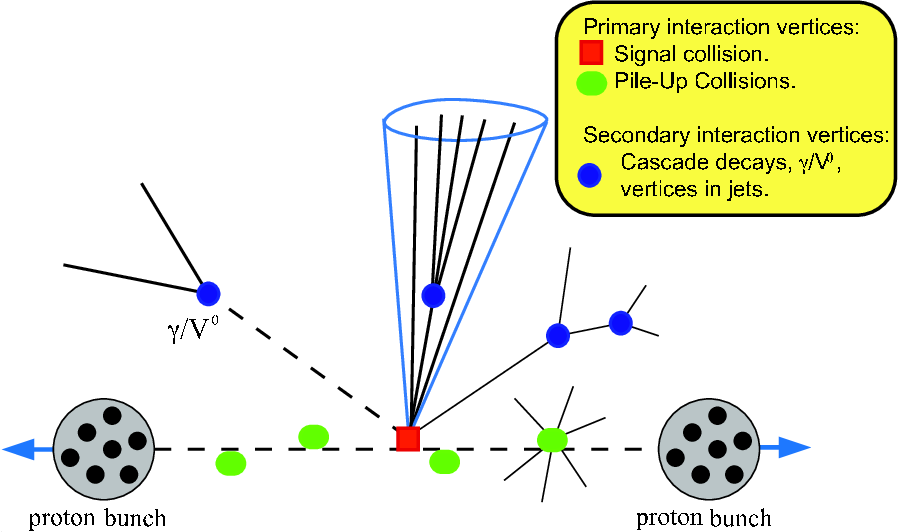
\includegraphics[width=0.45\textwidth]{plots/Vertices.png} 
  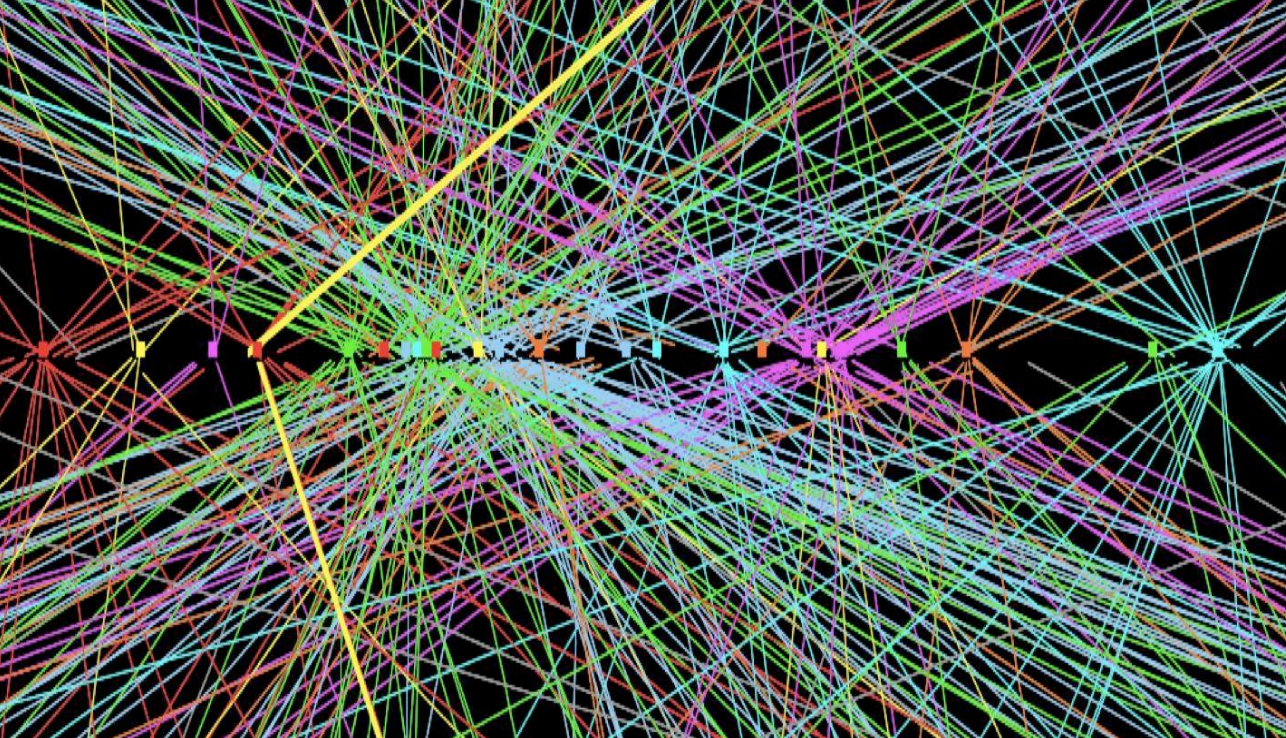
\includegraphics[width=0.45\textwidth]{plots/Vertices2.png} 
  \caption{Left: Diagram of the collision of proton bunches producing several vertices: one primary vertex from a rare interesting particle, and several pile-up vertices~\cite{ATLASVertices}. Right: Example of several vertices reconstructed in the ATLAS detector~\cite{TrackMLPPTBefore}.}
  \label{fig:Vertices}
\end{figure}

\ \\The second step is to reconstruct charged particle tracks. For example, an electron is reconstructed as a track in the ID, plus an electromagnetic shower in the EMCal. A muon is reconstructed as a track in the ID, plus energy deposits in the muon detector. A charged hadron is reconstructed as a track in the ID, plus a hadronic shower in HadCal. 

%\ \\Tracking is also key to reconstruct bottom ($b$) quarks. Top quarks decay about 100\% of the time into a $W$ boson and a $b$ quark. The Higgs boson decays most often (about 60\% of the time) to bottom-quark pairs. Also many supersymmetric particle decay signatures contain a $b$ quark. Identifying jets originating from bottom quarks is called \emph{b-tagging}. $b$-tagging uses tracks originating from the same vertex to identify a secondary vertex produced by the $B$-hadron decay after it has travelled about 3 mm away from the primary vertex.

\ \\Current tracking algorithms employed at ATLAS~\cite{TrackingATLAS} and CMS~\cite{TrackingCMS} use a combinatorial approach. First a track seed is found and later the track is computed. These algorithms require many calculations and thus require high CPU consumption. There is a stringent need to find algorithms with reduced CPU consumption to allow scaling from an LHC pile-up of about $\mu=36$ in Run-2 to $\mu=200$ in Run-3 and beyond. As illustrated in Figure~\ref{fig:CPU} (left), the CPU consumption increases more than quadratically with $\mu$. Tracking represents the largest part of the event reconstruction CPU. Figure~\ref{fig:CPU} (right) illustrates how the CPU consumption increases even further for Run-4 and Run-5. Especially for Run-4, scheduled for 2026, significant algorithm improvements are needed to improve tracking CPU requirements by a factor of approximately 10~\cite{TrackMLPPTBefore}.

%The CPU requirement increases further with increasing pile-up ($\mu$), due to the increased number of combinations of hits. Alternative more efficient algorithms are needed. In this thesis a machine learning algorithm is studied to reconstruct tracks at $\mu=200$ for the Run-3 through Run-5 at the LHC, using simulated data from the Particle Tracking Machine Learning Challenge, described in Chapter~\ref{chapter:TrackML}.

\begin{figure}[htb]
\centering
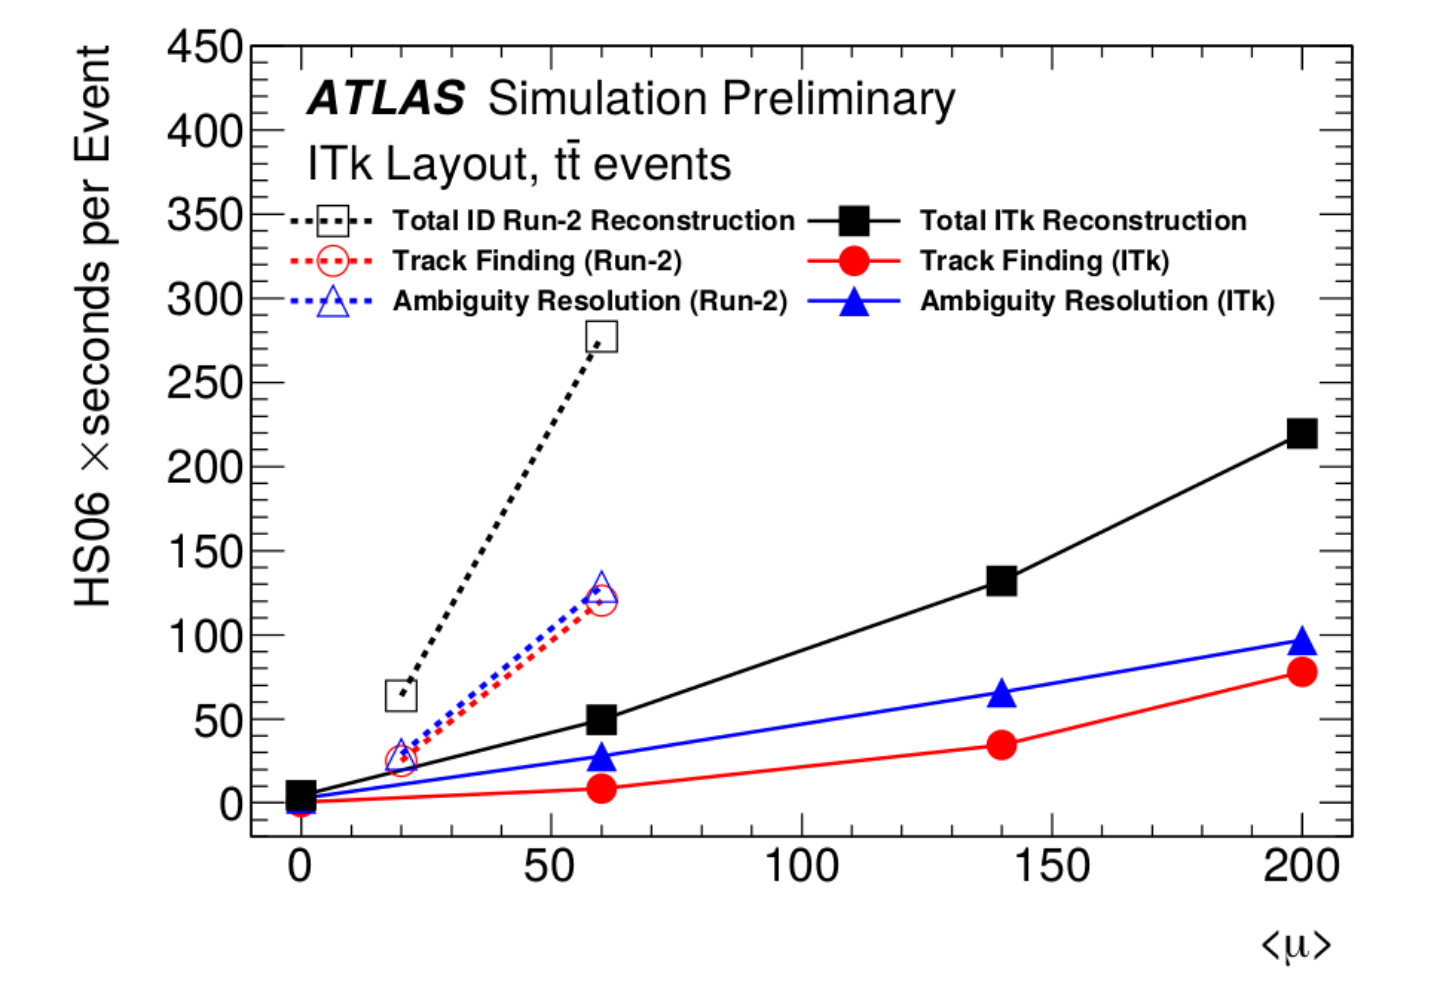
\includegraphics[width=0.45\textwidth]{./plots/CPU1.png}
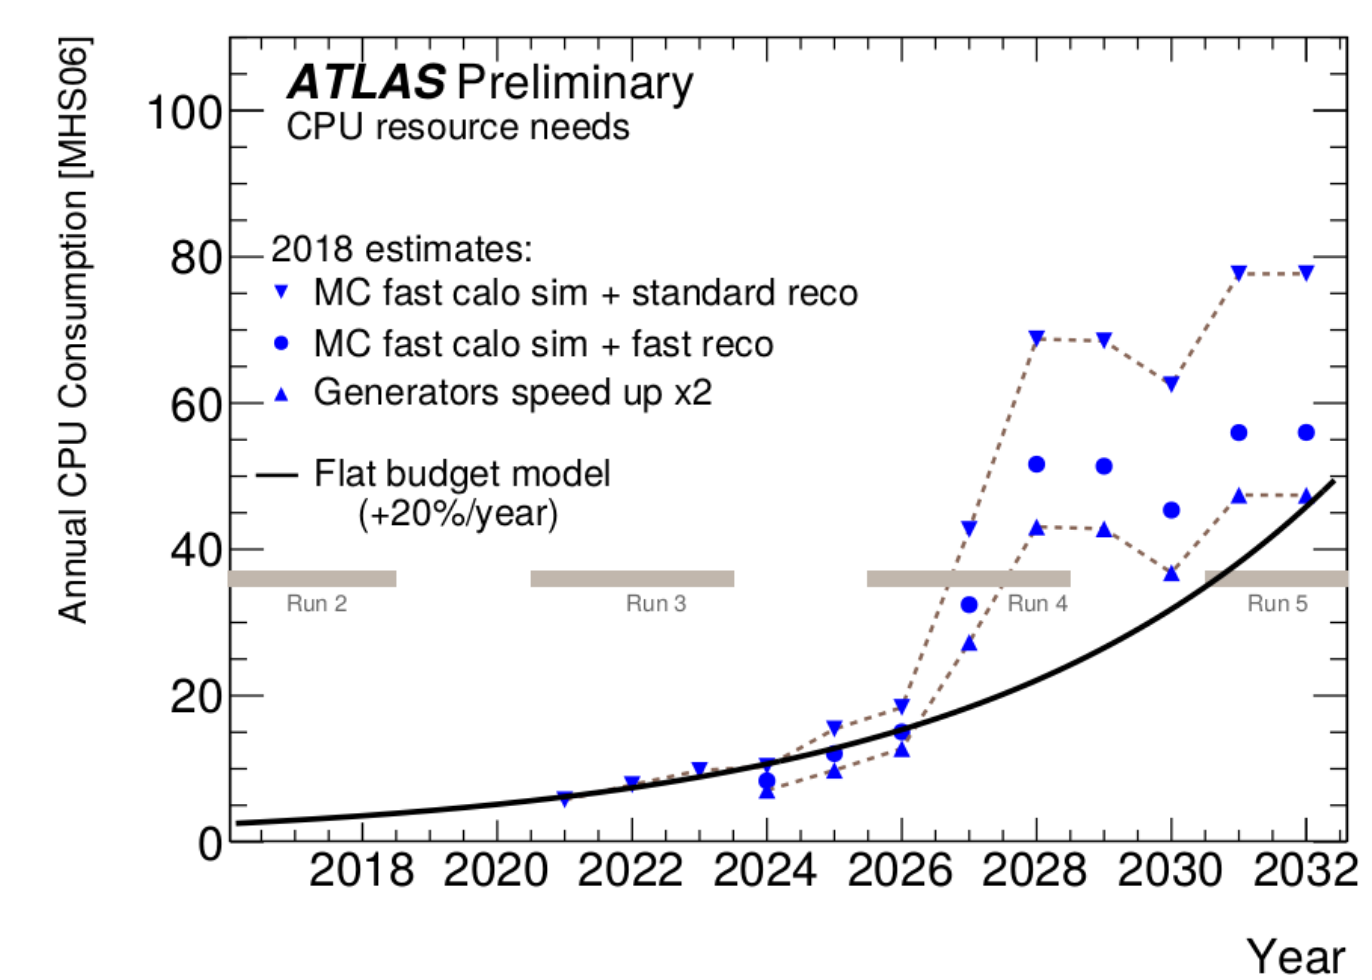
\includegraphics[width=0.45\textwidth]{./plots/CPU2.png}
\caption{CPU consumption increases more than quadratically with both pile-up (left) and years (right)~\cite{TrackMLPPTAfter}~\cite{TrackMLPPTAfter2}.}
\label{fig:CPU}
\end{figure}

\ \\A promising avenue is machine learning algorithms. Such algorithms require a lot of training data and require a long time to train (learn), but are usually fast to predict (infer). The field of machine learning has experienced a rapid growth in last few years. In this thesis a deep neural network algorithm is studied.

\chapter{TrackML}
\label{chapter:TrackML}

\section{TrackML Challenge}

To bring expertise for particle tracking for Run-3 to CERN from the computer science and machine learning communities, several LHC experiments have worked together to invite machine learning teams from outside CERN to compete in the 2018 Kaggle challenge called the TrackML Particle Tracking Challenge~\cite{TrackML}~\cite{TrackMLPPTBefore}~\cite{TrackMLPPTAfter}~\cite{TrackMLPPTAfter2} and a follow-up challenge in 2019~\cite{TrackML2}.

\ \\The candidates were offered a dataset of simulated charged particles in a general-purpose detector, representative of ATLAS and CMS at CERN. The simulation contains both the true and reconstructed position of the track hits, allowing for a labelled dataset on which learning can be performed. The dataset was obtained using a common tracking software framework at CERN called ACTS~\cite{ACTS}~\cite{ACTSPPT}. Events of top quark production (\ttbar~events) were simulated at $\mu=200$, leading to about 10 thousand tracks per event. \ttbar~events are known to produce many particles and consequently also many tracks. 

\ \\Tracks are reconstructed in the inner detector, which is simulated to be formed of three types of silicon detectors, to be representative of both the ATLAS and CMS at the planned High Luminosity LHC (HL-LHC). As illustrated in Figure~\ref{fig:ThreeSiDetectors}, the three silicon detectors are the pixels, short strips and long strips, in order of increasing radius. 

\begin{figure}[htb]
\centering
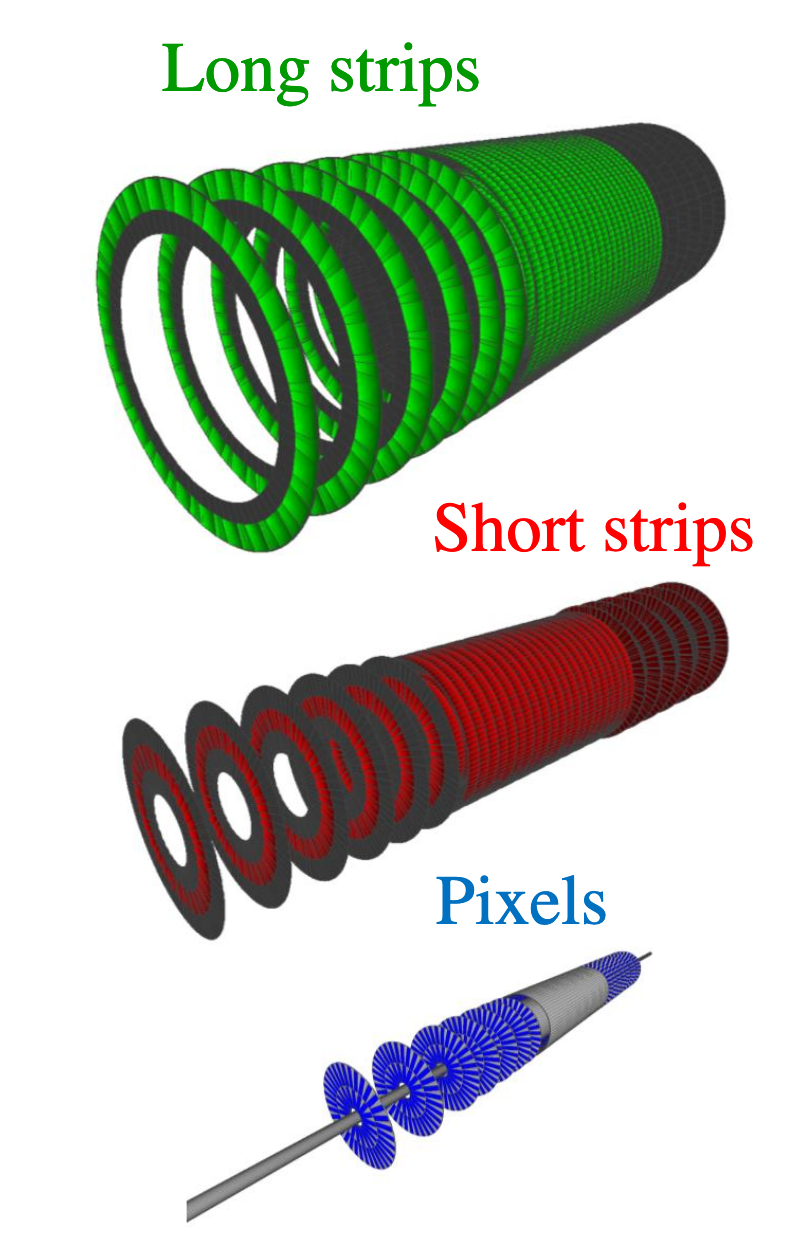
\includegraphics[width=0.45\textwidth]{./plots/ThreeSiDetectors.png}
\caption{Tracks are reconstructed in the inner detector, which is simulated to be formed of three types of silicon detectors. From beam pipe outwards the pixels, short strips and long strips~\cite{TrackMLPPTBefore}~\cite{TrackMLPaperAccuracyPhase}.}
\label{fig:ThreeSiDetectors}
\end{figure}

\ \\The coordinate system is right-handed and cartesian. The z-axis points along the beam axis (longitudinal axis). The x-y plane is the transverse plane. The azimuthal angle $\phi$ with values within $[0, 2\pi)$ is the angle in the transverse plane to the x-axis. The polar angle $\theta$ with values within $[0, \pi]$ is the angle to the z-axis. In particle physics, instead of the angle $\theta$ often the pseudo-rapidity $\eta$ is used, where $\eta = -\ln \tan (\theta/2)$.

\ \\In this coordinate system, the three silicon detectors are presented in the longitudinal plane in the left side of Figure~\ref{fig:DetectorGeometry}. The horizontal lines represent the barrel, and the vertical lines represent the two end-caps of the detector. The pixel detector is shown in the transverse plane in the right side of~\ref{fig:DetectorGeometry}. 

\begin{figure}[hbt]
\centering
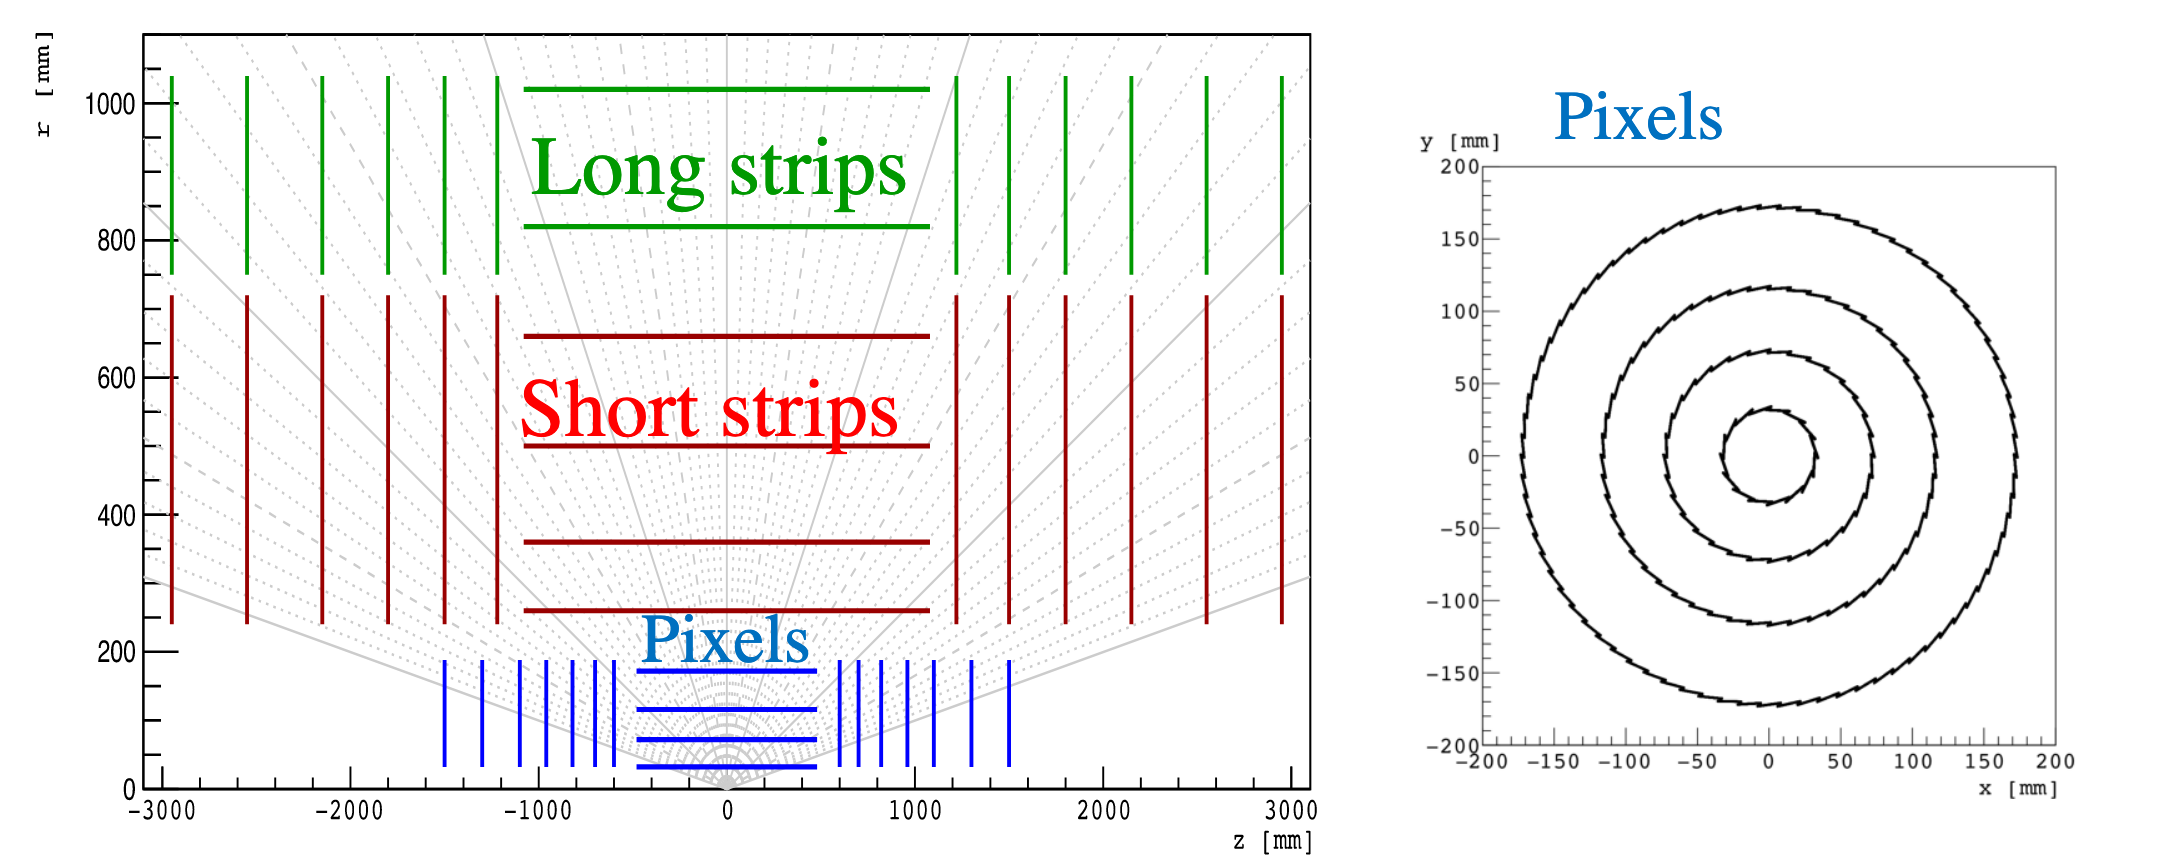
\includegraphics[width=0.9\textwidth]{./plots/DetectorGeometry.png}
\caption{The three detectors are organized in volumes, layers and modules~\cite{TrackMLPPTBefore}~\cite{TrackMLPaperAccuracyPhase}.}
\label{fig:DetectorGeometry}
\end{figure}

\section{Dataset}

Ten thousand events were simulated with collisions in the centre of the detector, leading to about 0.1 billion tracks. Each track has about 10 hits, or 3D points, in the simulated detector, leading to a total of 1 billion points, and about 100 GBytes of data~\cite{TrackMLPPTAfter2}. The dataset from TrackML is described in detail in~\cite{TrackMLPaperAccuracyPhase}~\cite{TrackMLPaper}~\cite{TrackMLPaperHAL}. A subset of 100 events of the TrackML dataset is used in this study.

\ \\The detector volumes for barrel and end-caps are divided into unique \volumeID. Each volume is divided into layers described by \layerID, which for technical reasons have only even values. Each layer is divided into modules identified by \moduleID. For each event, four files are provided~\cite{TrackMLPaper}, as described below.

\ \\The \emph{hit} file contains the reconstructed hit information: \hitID, the numerical identifier of the hit within the event, the measured coordinates $x$, $y$, $z$ of the hit in mm, the \volumeID, the \layerID, and the \moduleID.

\ \\The \emph{truth} file contains the generated (also called truth) hit information: the \hitID, the \particleID~of the particle that generated this hit, the truth coordinates $tx$, $ty$, $tz$ in mm, and the truth momenta $tpx$, $tpy$, $tpz$. 

\ \\The \emph{particles} file contains for each \particleID~the particle type, its velocities and momenta, the electric charge and the number of hits.

\ \\The \emph{cells} file contains for each \hitID~the cell that recorded the hit. A cell is the smallest unit in a particle detector. A cell is identified uniquely by two channel numbers, similarly to two coordinates of a pixel in an image. 

\ \\In this thesis only the \emph{hit} and \emph{truth} files of 100 events simulated with $\mu=200$ are studied. They are read in as data frames, and concatenated by columns. As a result, for each \hitID~one knows the reconstructed coordinates, the truth coordinates, truth momenta and to what \particleID~it belongs to. 

\section{Simulated Truth Particles and Reconstructed Hits}

One random event with index 99 is studied. Its behaviour is however representative for all events. A typical event produces about 10 thousand simulated particles, with a distribution of the number of hits per particle illustrated in Figure~\ref{fig:TruthParticleNbHits}, with a mean of 10.8 and a standard deviation (rms) of 3.3.

\begin{figure}[htb]
\centering
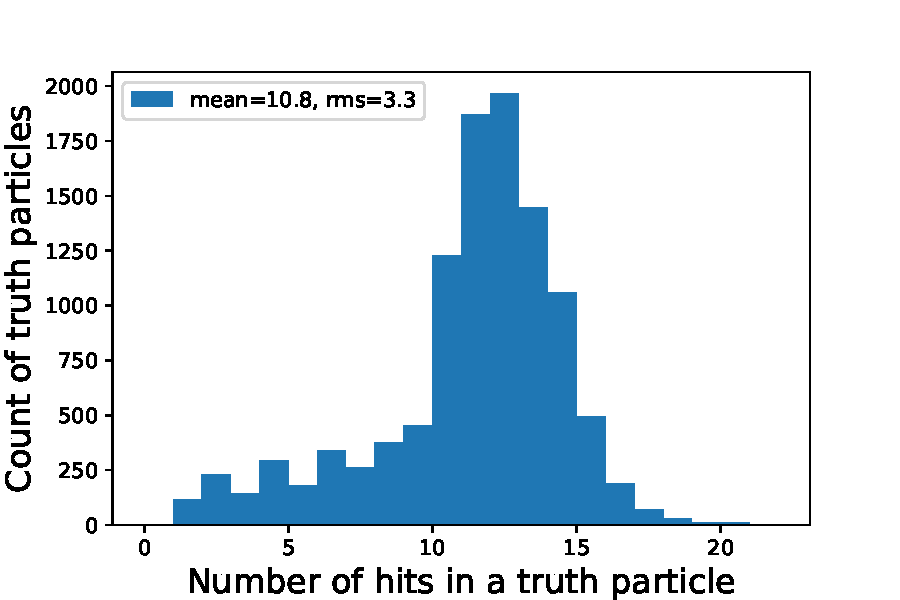
\includegraphics[width=0.45\textwidth]{plots/DataExploration_histo_counterTruthParticles_vs_nbHitsInTruthParticle.pdf}
\caption{Distribution of the number of hits in truth particles in event 99}
\label{fig:TruthParticleNbHits}
\end{figure}

%\ \\All collisions are simulated in the center of the detector, and all particles emerge from very close to the center of the detector. There are no particles travelling far away from the center of the detector, which is represented physically by no cosmic ray particles being considered in the sample. To double check this, for each truth particle of event 99, the $r$ and $z$ coordinates of all hist belonging to the particle are fit to a straight line of equation $y=a_0+a_1x$. $a_0$ is the $r$ value at $z=0$, while $a_1$ is the tangent of the slope angle. $z_0 = -a_0/a_1$ is the $z$ coordinate at zero radius $r$. Both $a_0$ and $z_0$ should be very close to zero for particles simulated in the center of the detector, and have large values for cosmic particles. Their distribution, illustrated in Figure~\ref{fig:TruthParticleFit} confirm that indeed there are no cosmic particle and all particles are simulated in the center of the detector. Furthermore, the angle of the particles peaks at -90 and 90 degrees, meaning that most particles are emitted in the transverse plane. Indeed, it is expected from a so called hard-scatter collision, like the \ttbar~events simulated for TrackML.

%\begin{figure}[!htb]
%\centering
%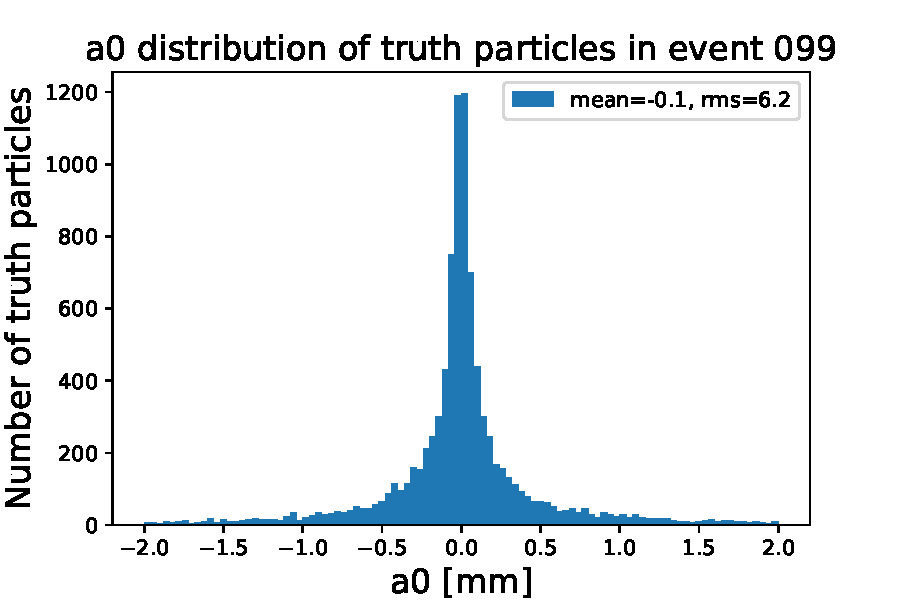
\includegraphics[width=0.45\textwidth]{plots/DataExploration_a0.pdf}
%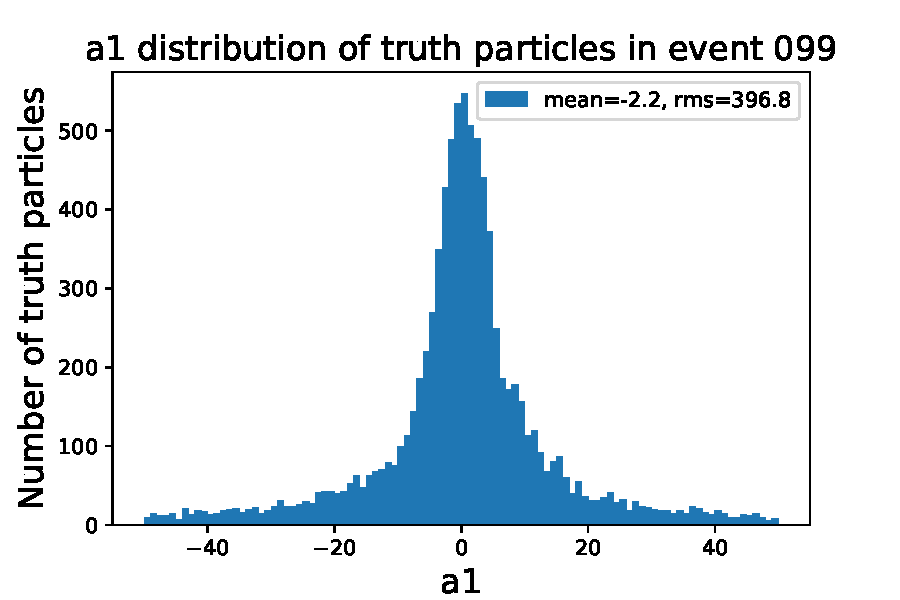
\includegraphics[width=0.45\textwidth]{plots/DataExploration_a1.pdf}\\
%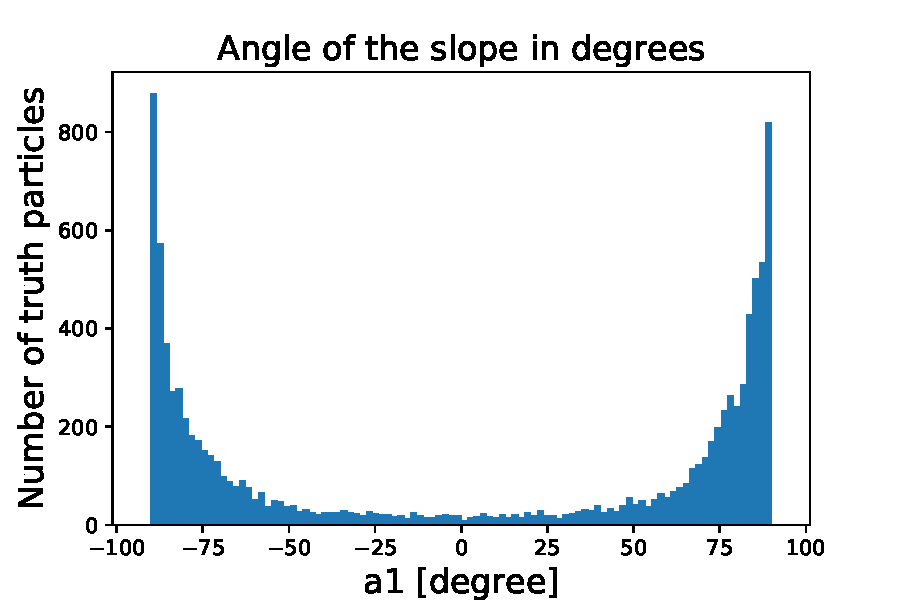
\includegraphics[width=0.45\textwidth]{plots/DataExploration_a1_degree.pdf}
%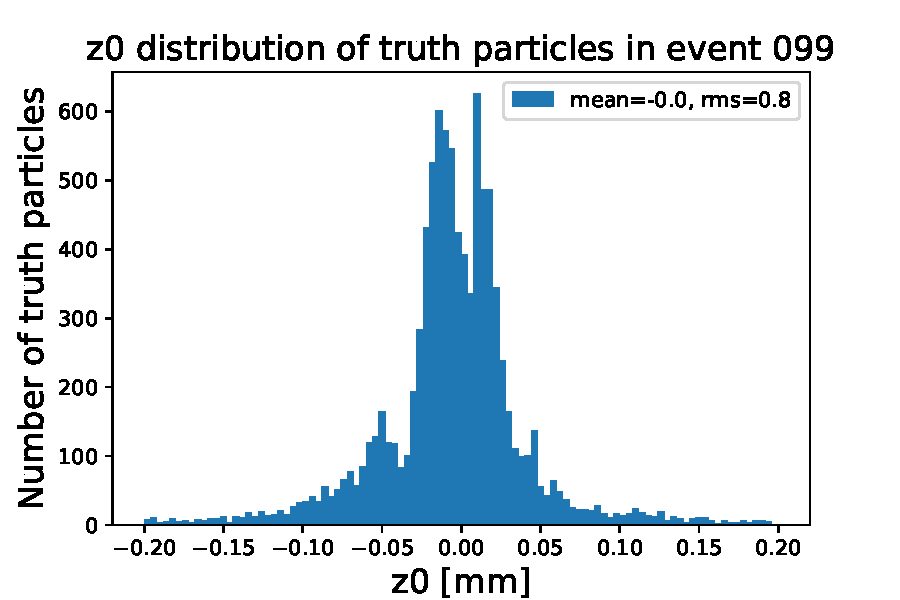
\includegraphics[width=0.45\textwidth]{plots/DataExploration_z0.pdf}
%\caption{$a_0$ [mm], $a_1$,  $a_1$ [degree], $z_0$ [mm] distributions for all truth particles in event 99.}
%\label{fig:TruthParticleFit}
%\end{figure}

\ \\Particles produced in the collisions in the centre of the detector travel in all possible directions. Four tracks made of hits for truth particles, going to both left and right, at an angle closer to the transverse plane, or to the z-axis, are shown in Figure~\ref{fig:TruthParticleTracks}. The images confirm that the hits for each particle are grouped along a line. The $z$ and radius $r$ coordinates are fit to a line of equation ($r = a_0 + a_1 \cdot x$). $a_0$ represents the intercept, or the radius when $z=0$, at the centre of the detector. The values of $a_0$ that are close to zero are consistent with the particles being emitted from the centre of the detector. $a_1$ represents the slope of the line. The fact that $a_0$ have different values, both positive and negative, show that particles are emitted in all directions. $z_0$ represents the $z$ position when the radius $r=0$, meaning when the particle line intersects the z-axis. The fact that the $z_0$ values are close to zero is consistent again with the particles being emitted in the centre of the detector.

\begin{figure}[htb]
\centering
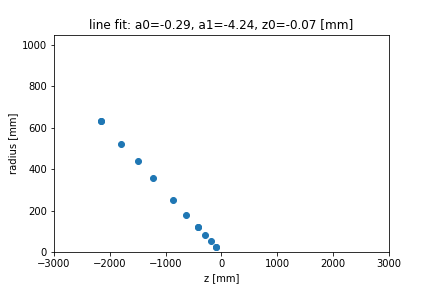
\includegraphics[width=0.35\textwidth]{plots/particle_553945090628780032_r_vs_z.png}
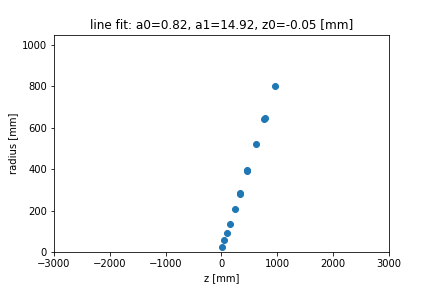
\includegraphics[width=0.35\textwidth]{plots/particle_540433329673994240_r_vs_z.png}\\
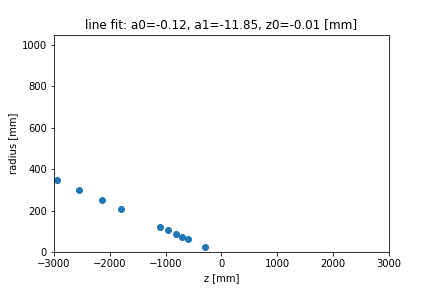
\includegraphics[width=0.35\textwidth]{plots/particle_94575729613733888_r_vs_z.png}
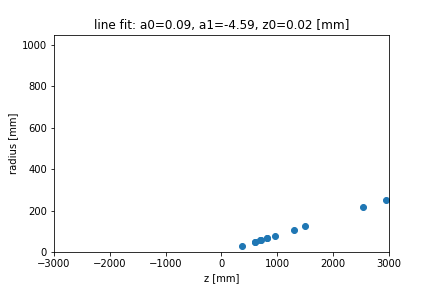
\includegraphics[width=0.35\textwidth]{plots/particle_99081047228022784_r_vs_z.png}
\caption{Four truth particle tracks from event 99 travelling in all possible directions shown in the longitudinal r-z plane. A straight line of equation $r = a_0 + a_1 \cdot x$ is fitted to the points. $a_0$ is the intercept and $a_1$ is the slope. $z_0$ is the $z$ coordinate when the radius $r=0$.}
\label{fig:TruthParticleTracks}
\end{figure}

%\section{Reconstructed hits}
\ \\The reconstructed hit coordinates $x$, $y$, $z$ are very close to the corresponding truth values, as illustrated in Figure~\ref{fig:ReconstructedToTruthHits}. The reconstructed scale and resolution values are therefore good. 

\begin{figure}[htb]
\centering
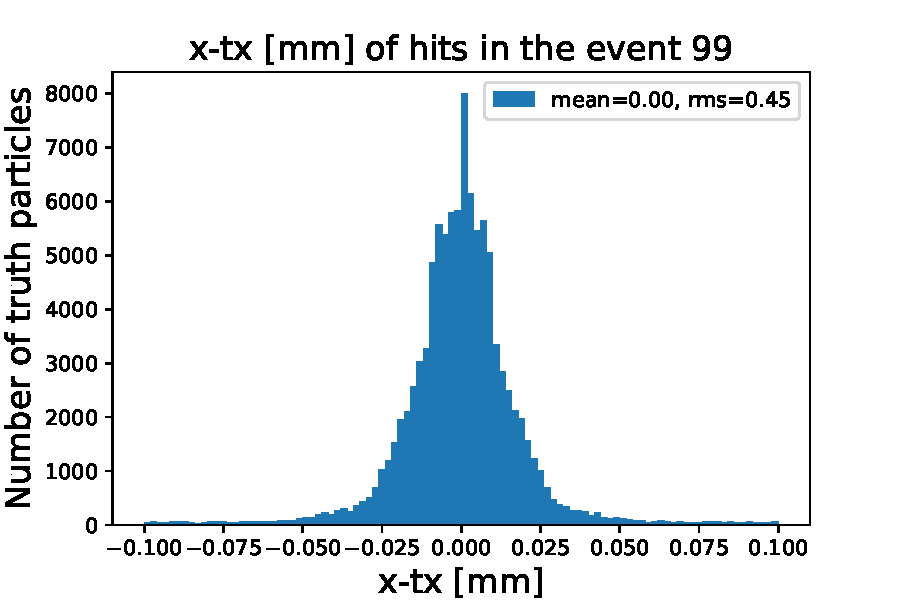
\includegraphics[width=0.32\textwidth]{plots/DataExploration_x_tx.pdf}
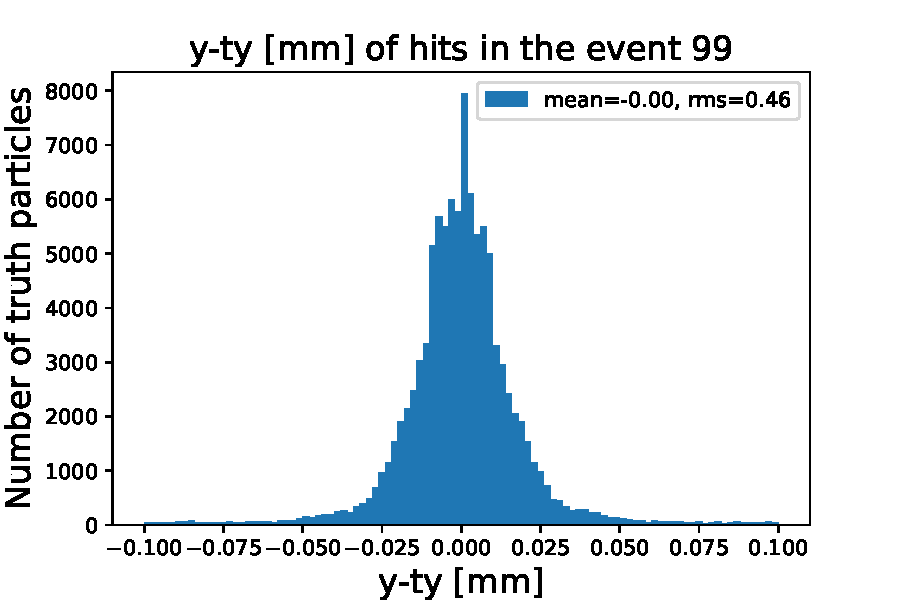
\includegraphics[width=0.32\textwidth]{plots/DataExploration_y_ty.pdf}
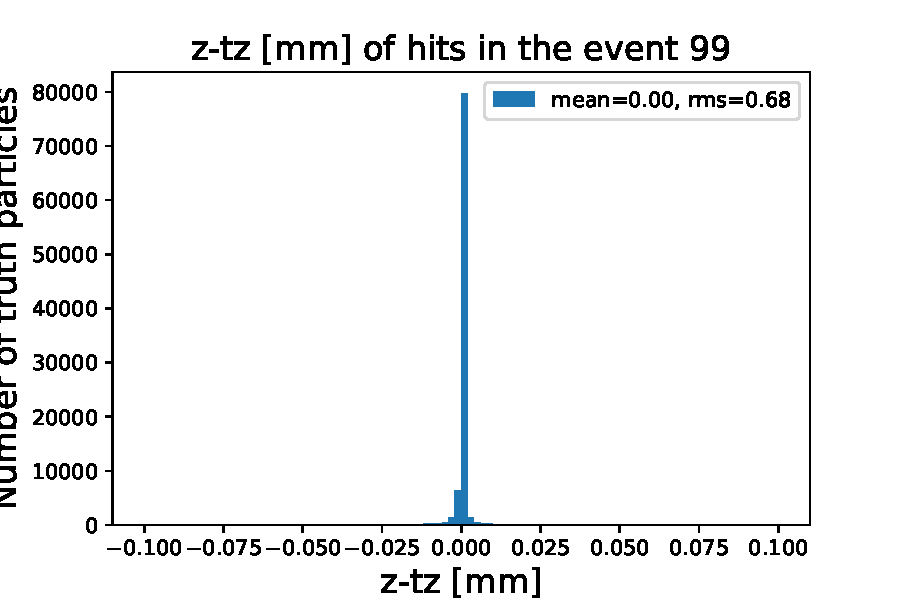
\includegraphics[width=0.32\textwidth]{plots/DataExploration_z_tz.pdf}
\caption{Distributions of reconstructed values minus truth values for $x$, $y$, $z$ in mm for all truth particles in event 99}
\label{fig:ReconstructedToTruthHits}
\end{figure}

\ \\Their coordinates, plus the $r$ coordinate, are illustrated in Figure~\ref{fig:ReconstructedHits}. 

\begin{figure}[htb]
\centering
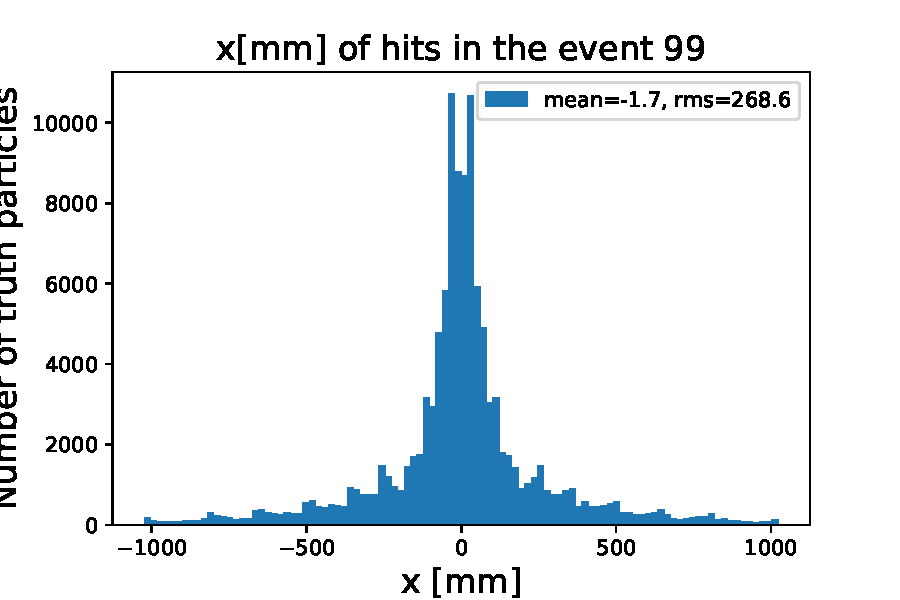
\includegraphics[width=0.35\textwidth]{plots/DataExploration_x.pdf}
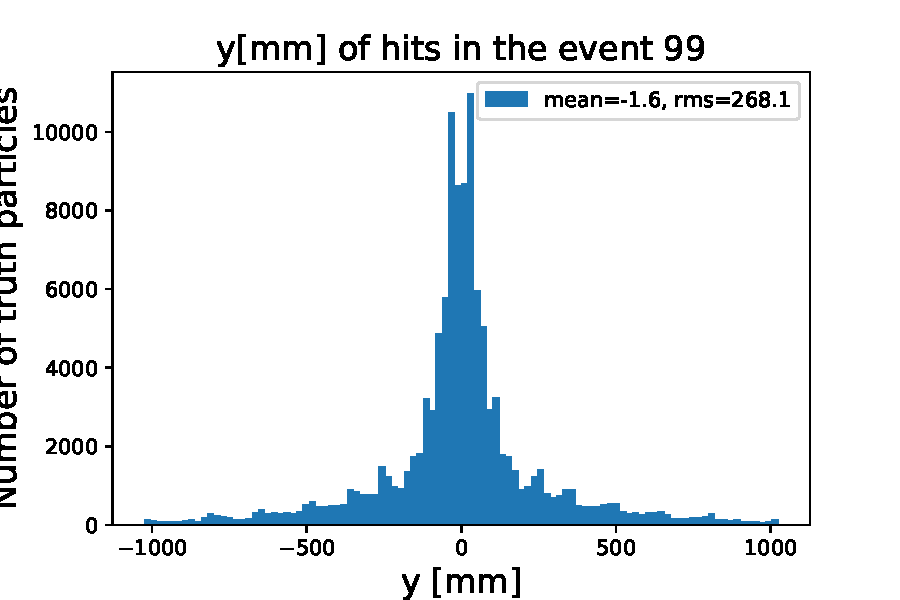
\includegraphics[width=0.35\textwidth]{plots/DataExploration_y.pdf}\\
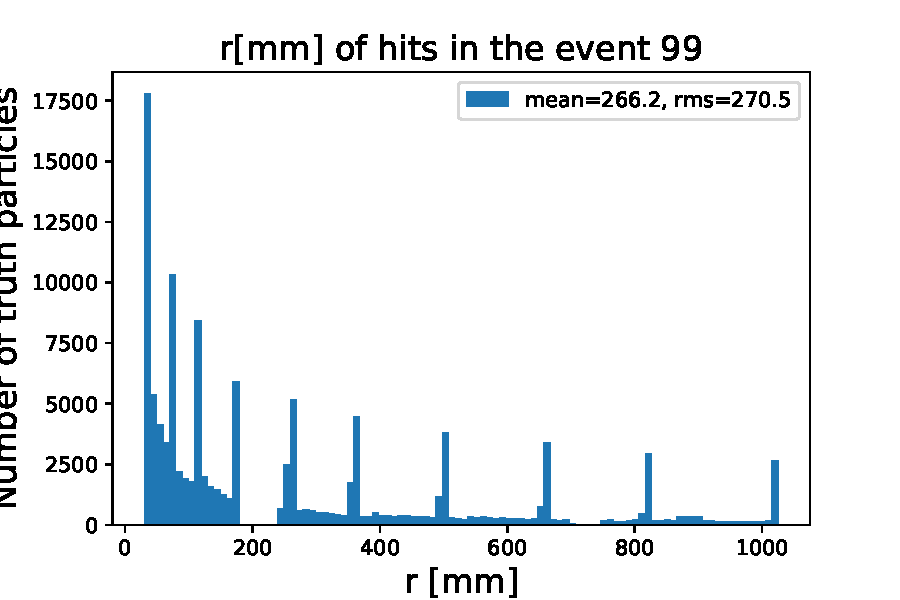
\includegraphics[width=0.35\textwidth]{plots/DataExploration_r.pdf}
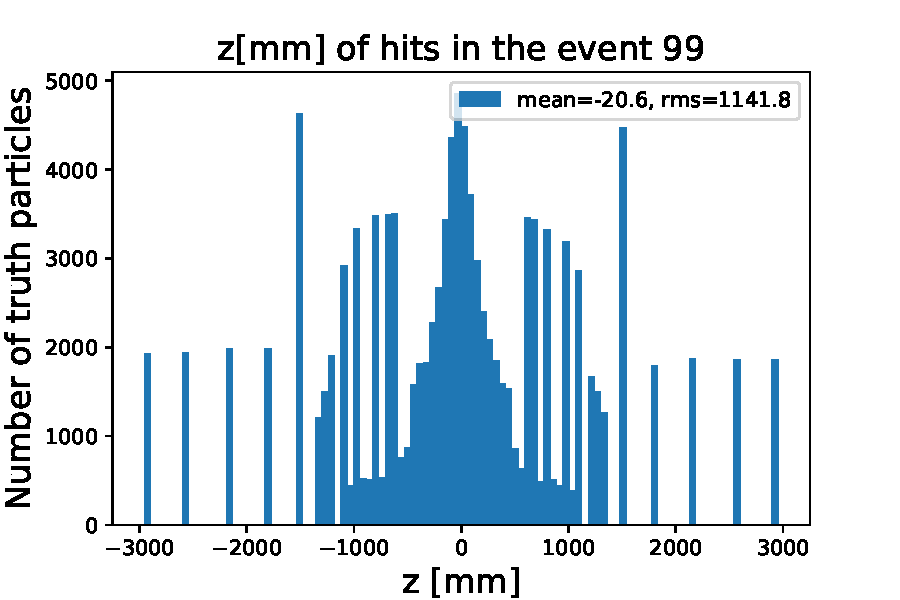
\includegraphics[width=0.35\textwidth]{plots/DataExploration_z.pdf}
\caption{$x$, $y$, $r$, $z$ distributions in mm for all truth particles in event 99}
\label{fig:ReconstructedHits}
\end{figure}

\section{Detector Components}

The grouping of hits inside the detector is used later in this study to evaluate the performance of the model in each detector sub-volume called \volumeID. The detector is formed by a central barrel and two end-caps. There are three layers of volumes from the beam outwards. The volumes from the barrel (end-caps) have the modules alligned horizontally (vertically). Most hits are detected in the volumes of the inner layer, and in those of the barrel. This is consistent with hard-scatter collisions emitted mostly at high $\pt$, so close to the transverse plane. The \volumeID~numbers are visualised in Figure~\ref{fig:DetectorVolumeIDLayerID}, along with the percentage of the hits in each \volumeID, as measured in 100 simulated event in this study. Also Figure~\ref{fig:DetectorHits} illustrates the clustering of hits by \volumeID, \layerID, and \moduleID. The 2D scatter plots between the \volumeID~and the \moduleID~on one side and the $r$ and $z$ on the other side are illustrated in Figure~\ref{fig:ScatterPlotHits}. 

\begin{figure}[!hbt]
\centering
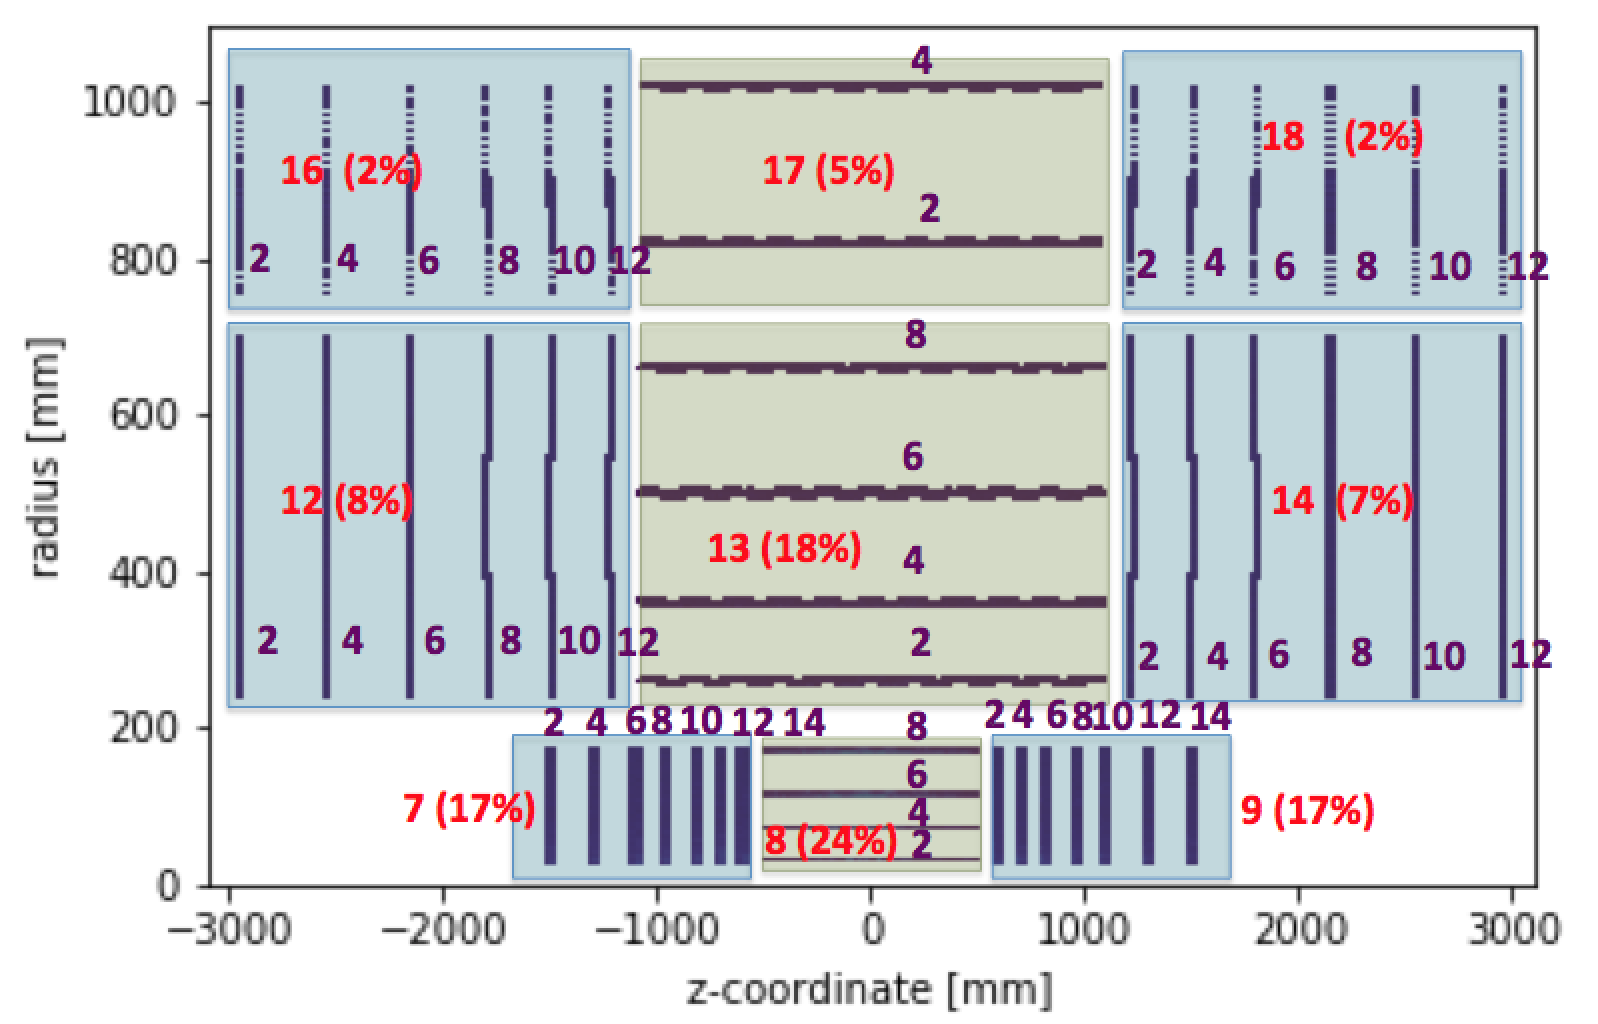
\includegraphics[width=0.9\textwidth]{./plots/DetectorVolumeIDLayerID.png}
\caption{Percentage of hits from 100 events in each volume ID and layer ID}
\label{fig:DetectorVolumeIDLayerID}
\end{figure}

\begin{figure}[!htb]
\centering
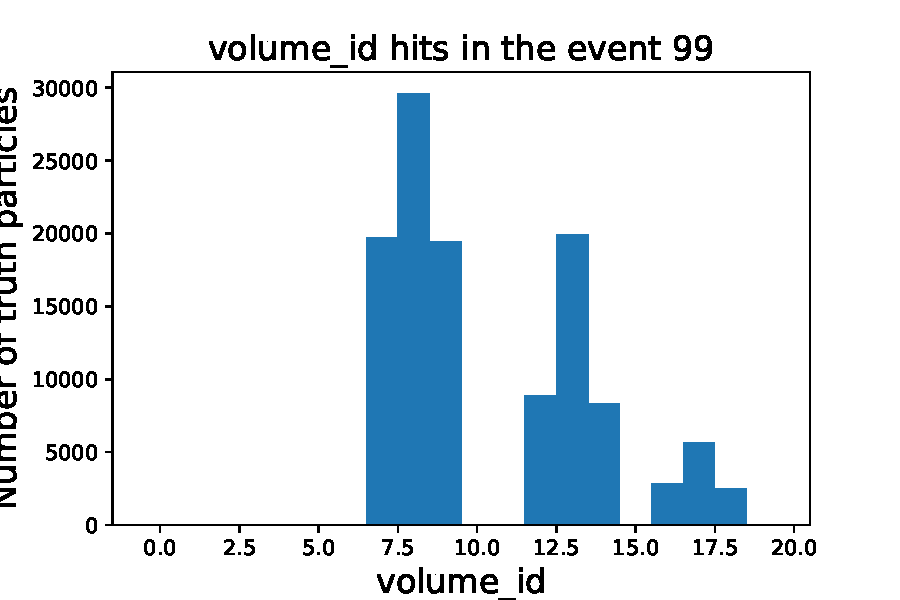
\includegraphics[width=0.32\textwidth]{plots/DataExploration_volume_id.pdf}
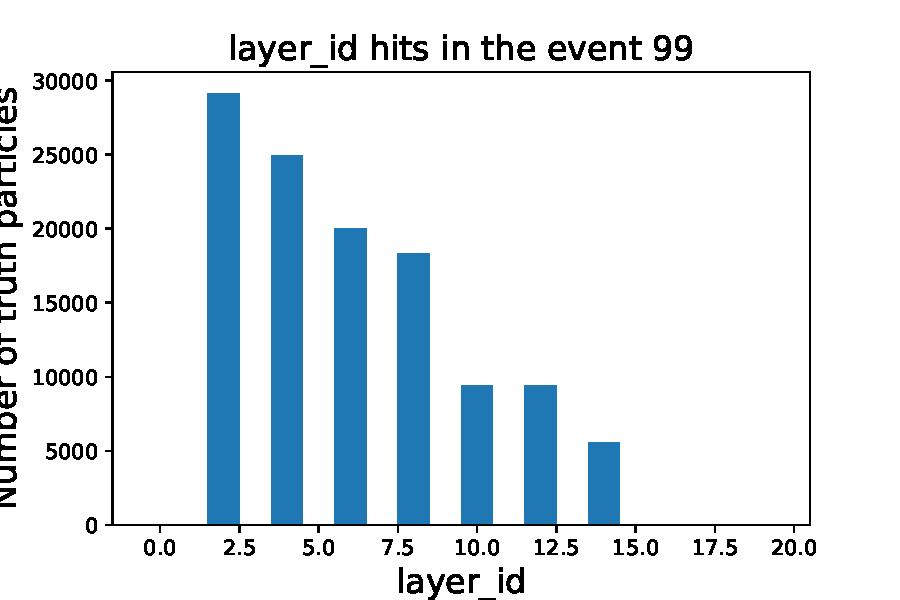
\includegraphics[width=0.32\textwidth]{plots/DataExploration_layer_id.pdf}
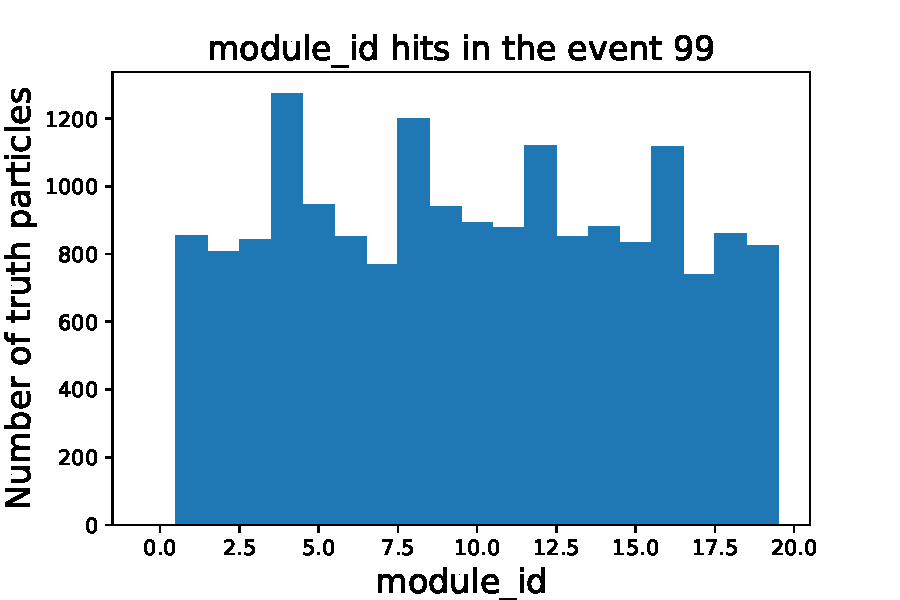
\includegraphics[width=0.32\textwidth]{plots/DataExploration_module_id.pdf}
\caption{Distributions of reconstructed hits in the various volume ID, layer ID and module ID, for all truth particles in event 99}
\label{fig:DetectorHits}
\end{figure}

\begin{figure}[!htb]
\centering
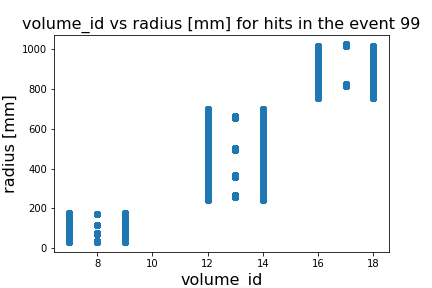
\includegraphics[width=0.35\textwidth]{plots/DataExploration_volume_id_r.png}
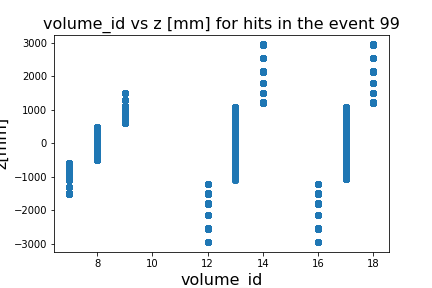
\includegraphics[width=0.35\textwidth]{plots/DataExploration_volume_id_z.png}\\
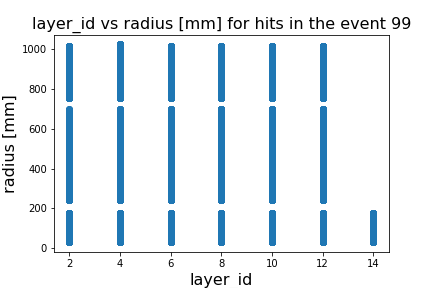
\includegraphics[width=0.35\textwidth]{plots/DataExploration_layer_id_r.png}
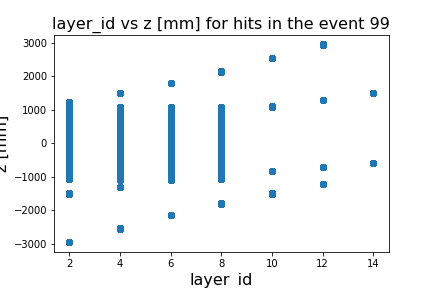
\includegraphics[width=0.35\textwidth]{plots/DataExploration_layer_id_z.png}
\caption{2D scatter plots of the reconstructed hits between the volume ID, module ID versus $r$ and $z$ coordinates, for all truth particles in event 99}
\label{fig:ScatterPlotHits}
\end{figure}

%\ \\ The distribution for one event of the \volumeID~and the \moduleID~inside the detector is illustrated in Figure~\ref{fig:ScatterRZ}.
%
%\begin{figure}[!htb]
%\centering
%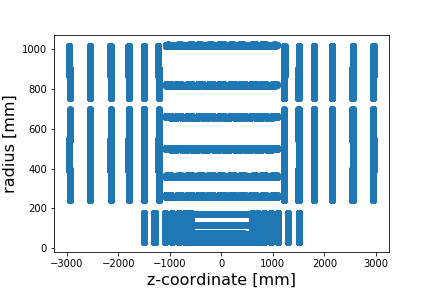
\includegraphics[width=0.7\textwidth]{plots/DataExploration_z_vs_r_scatter.png}
%\caption{2D scatter plots of the reconstructed hits between the $r$ and $z$, for all truth particles in event 99.}
%\label{fig:ScatterRZ}
%\end{figure}




\chapter{Problem Setting}
\label{chapter:ProblemSetting}

In this study a machine learning algorithm is developed to reconstruct tracks from reconstructed hits in an event. The dataset used is comprised of 100 events from the TrackML challenge, described in Chapter~\ref{chapter:TrackML}. This chapter describes what is processed for a given event, how are the input and output datasets formed, and how is the question formulated.

\section{Question}
\label{sec:Question}

Ideally, one would want like to take as input the totality of hits reconstructed in the detector in one event and return all the reconstructed particle tracks, each track with its own set of hits. This problem is too hard to solve due to the very large combinatorics. 

\ \\The problem may be simplified by asking to identify all the particle tracks in a given group of hits, also each particle with its own hits. It turns out this is still too hard. So an even simpler problem is attempted. 

\ \\In each group of reconstructed hits, there is one truth particle that has the largest number of hits in the group. This particle is denoted the \emph{majority particle} or the \emph{leading particle}. If a hit belongs to the majority particle, then it is assigned a label of 1 and is considered a positive hit (signal). If not, it is assigned a label of 0 or -1. In this study a label of -1 is used and it is considered a negative hit (background). The number of positive hits in the group represents physically the \emph{majority particle size} and is denoted by \nbPositiveHit. The question then becomes for each hit in the group if it belongs or not to the particle with the largest number of hits in the group (the majority particle). In other words, the question is given the x, y, z coordinates of all the hits in the group to predict the label of each hit in the group (1 or -1).

\section{Approximate Nearest Neighbours}
\label{sec:Approximate Nearest Neighbours}

A preliminary step is therefore to select groups of hits from the event that are close to each other in such a way as to be likely that the group contains at least one real particle inside. We employ an algorithm denoted \emph{approximate nearest neighbours}, a form of unsupervised learning, described in detail in Reference~\cite{BucketCreation}. The collection of hits with $x$, $y$, $z$ coordinates is represented mathematically by a 3D point cloud. 

\ \\Usually the distance considered to measure the closeness is the euclidean distance in 3D (x, y, z). However, in this case, it is best to select hits not closest in space, but closest to the same direction of travel from the centre of the detector onwards, as illustrated in Figure~\ref{fig:TruthParticleTracks} for several truth particles. Nearest neighbours can be computed exactly via brute force techniques, but they consume too many resources in terms of memory, CPU and time. Given the large number of hits in one event, it is preferred to use a more efficient algorithm, even if it may not return the exact result at every query. Such methods are called \emph{approximate nearest neighbour} methods. The algorithm contains two main steps, illustrated in Figure~\ref{fig:ApproximateNearestNeighbours}.

\begin{figure}[htb]
\centering
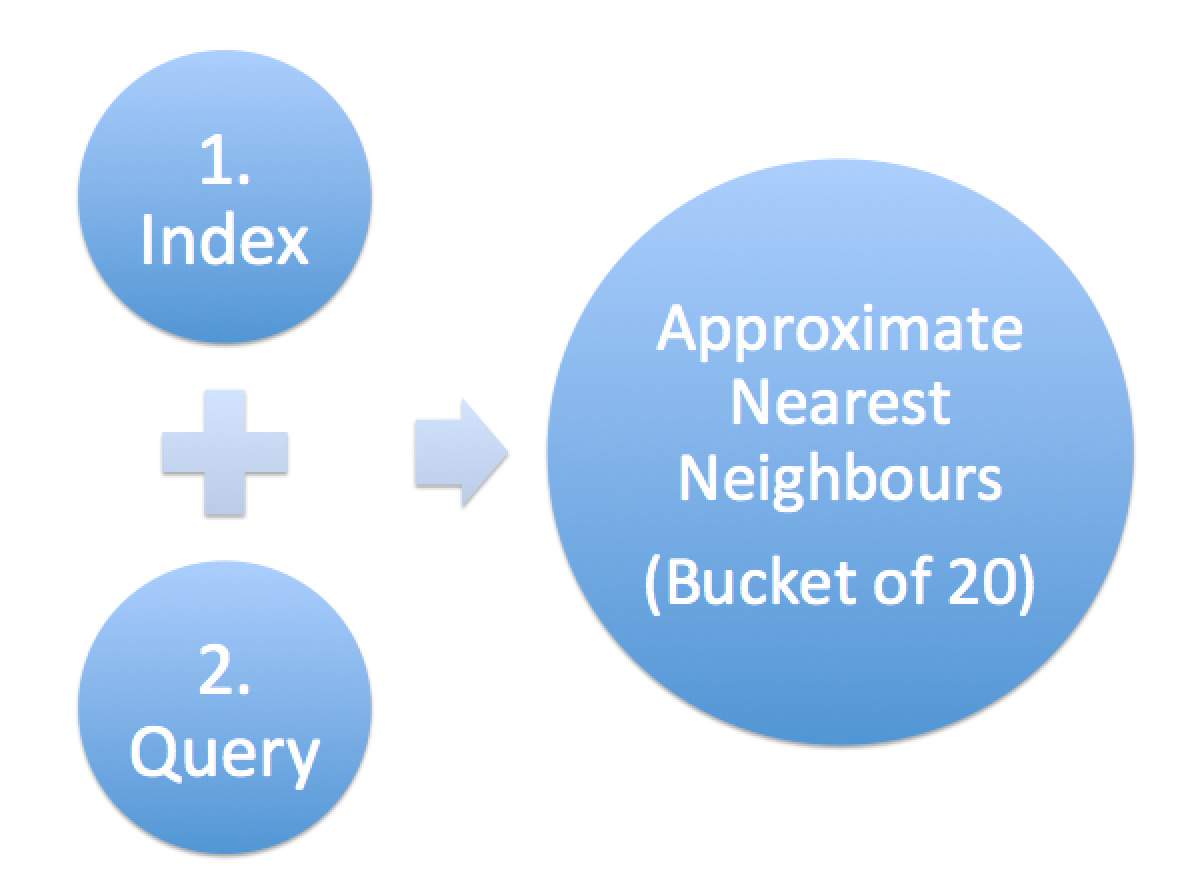
\includegraphics[width=0.35\textwidth]{./plots/ApproximateNearestNeighbours.jpeg}
\caption{There are two steps in the ApproximateNearestNeighbours. First create an index from the positions of all hits in the event. Then query hits (even in parallel) to find the nearest neighbours to each hit.}
\label{fig:ApproximateNearestNeighbours}.
\end{figure}

\ \\The first step takes as input the x, y, z coordinates of all the reconstructed hits in an event and returns as output a tree that groups the hits along their direction relative to the centre of the detector. The tree is built using random projections. At every node, a random sample of two hits is chosen and the hyper-plane equidistant to both hits is chosen to divide into two further subspaces. This is done k times, to obtain an ensemble method of a forest of trees. k is a hyper-paramter to tune and is set to 10 in our study. The result is called an index. 

\ \\In the second step, a query hit is given and the N-nearest-neighbour hits along the direction are returned (including the query hit), where N is a parameter choosen by the user. The resulting group of hits is called a \emph{bucket} or a \emph{hash} of hits. The operation is done for every hit in the event, resulting in as many buckets as hits in the event. The procedure is then repeated for each event in the sample.

\ \\There are several code implementations of the Approximate Nearest Neighbors algorithm. In this project the implementation in Annoy (Approximate Nearest Neighbors Oh Yeah)~\cite{Annoy} is used. Annoy is fast, since it is coded in C++, but easy to use from Python as it provides a Python wrapper (or bindings). Annoy is an efficient library as a static read-only file is produced for the index, allowing it to be queried simultaneously (in parallel) by many threads, like when running on several CPU cores, or a GPU, or in a real production environment. The Annoy implementation supports the two step process described above: building one tree and querying in parallel for several points.

\ \\The number N of hits in a bucket is chosen to be 20, since in Figure~\ref{fig:TruthParticleNbHits} the count of truth particles by the number of hits tails off just before 20. The pseudo-code used in this project to produce a bucket for each hit in each of the 100 events described in Appendix~\ref{sec:AppendixPseudoCodeInputOutput}.

\section{Buckets}
\label{sec:Buckets}

With the procedure above the distribution of the size of the majority particle, defined in Section~\ref{sec:Question} and denoted \nbPositiveHit, is obtained and illustrated in Figure~\ref{fig:BucketNbPositiveHit} for the Train and Test samples that are described later in Section~\ref{sec:TrainAndTest}. The mean and rms of the histograms are 8.5 and 2.8, respectively. The interpretation is that the average bucket contains fewer than 10 hits belonging to the same particle.  

\begin{figure}[htb]
\centering
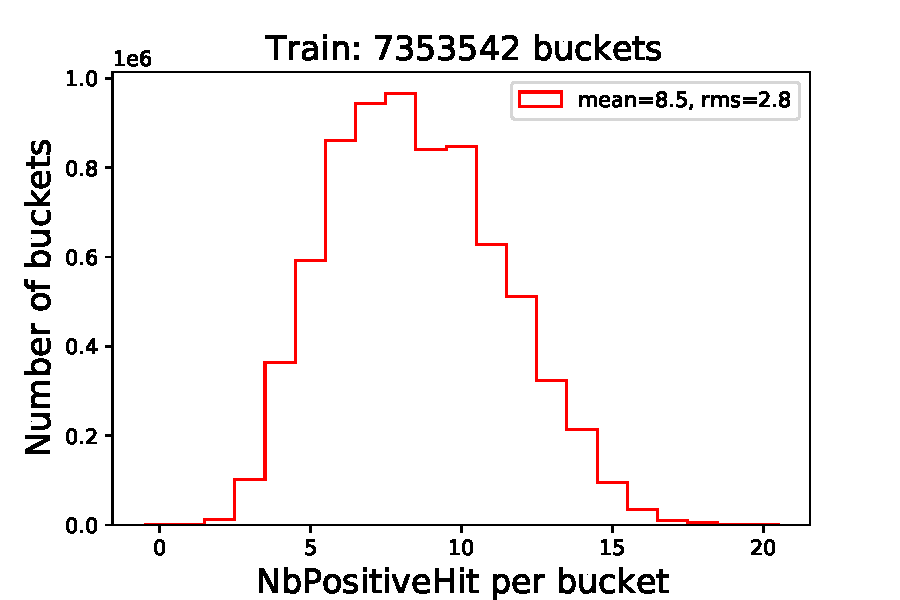
\includegraphics[width=0.34\textwidth]{plots/plot_bucket_unbalanced_Train_2.pdf}
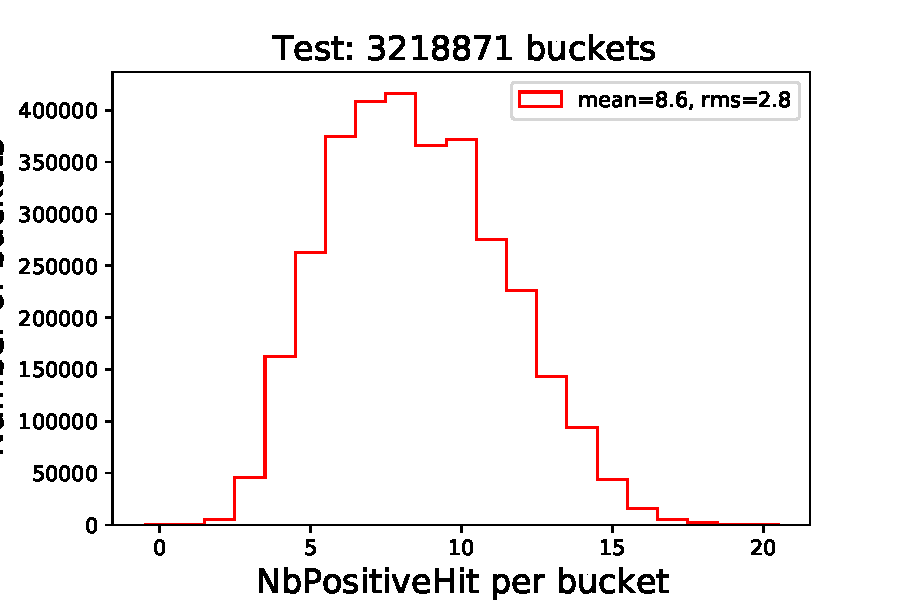
\includegraphics[width=0.34\textwidth]{plots/plot_bucket_unbalanced_Test_2.pdf}
\caption{The distribution of the majority particle size, or \nbPositiveHit.}
\label{fig:BucketNbPositiveHit}.
\end{figure}

\ \\Similarly as to the reconstructed hits above, another aspect realised from the Figure~\ref{fig:TruthParticleNbHits} is that only a fraction of truth particles have a number of hits smaller than 10. For both reasons, it is desired to reconstruct a particle with a significant number of hits in the bucket. A threshold of 10 is chosen. If a bucket has $\nbPositiveHit < 10$, then all its hit labels are set artificially to -1, leading to its $\nbPositiveHit=0$. In Figure~\ref{fig:BucketUnbalanced} the default threshold of 0 (Min00) and the chosen threshold of 10 (Min10) are overlaid for both the Train and Test samples. The Train and Test samples represent 70\% and 30\% of the events, respectively, as detailed in Section~\ref{sec:TrainAndTest}, and behave similarly. For each sample, the histograms for $\nbPositiveHit \ge 10$ are identical (seen as an overlapped colour). The values in red with  $\nbPositiveHit < 10$ appear in blue at $\nbPositiveHit = 10$. After this change the unbalance between the fraction of positive and negative hits is increased in the favor of the negative hits. A further balancing is needed, as described in Section~\ref{sec:BalancingDatasets}. 

\begin{figure}[htb]
\centering
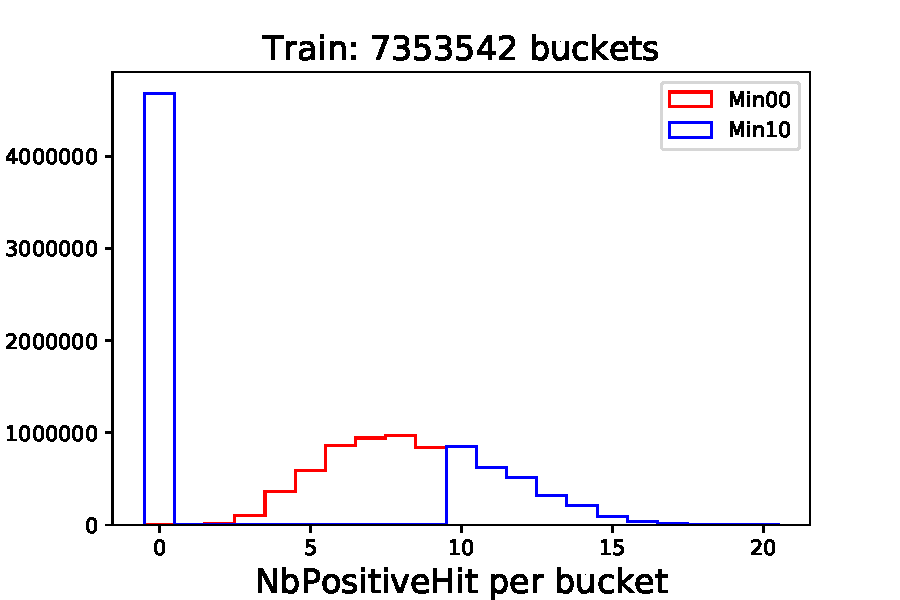
\includegraphics[width=0.34\textwidth]{plots/plot_bucket_unbalanced_Train.pdf}
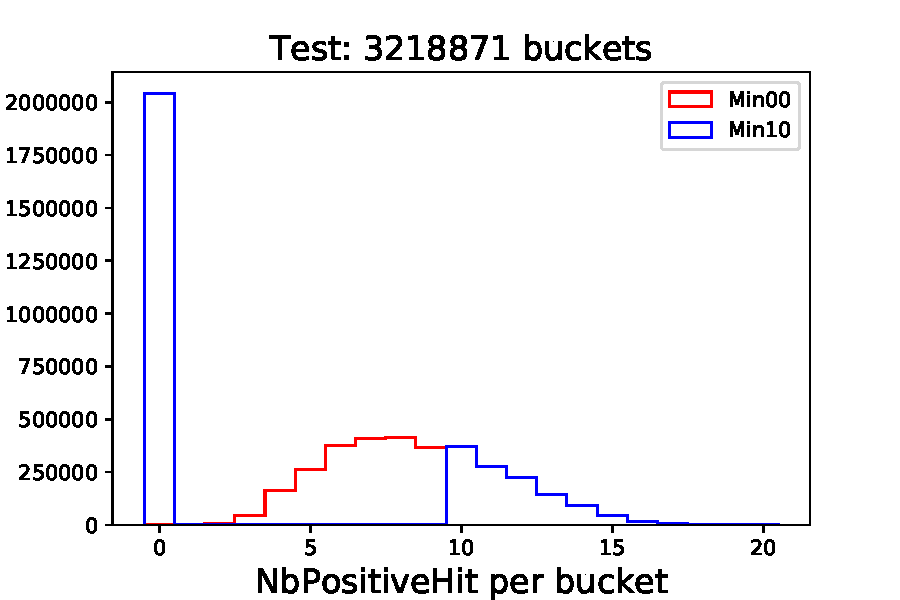
\includegraphics[width=0.34\textwidth]{plots/plot_bucket_unbalanced_Test.pdf}
\caption{Overlay of the number of positive hits per bucket by default (Min00) and after moving all hits to negative for buckets with less than 10 number of positive hits (Min10). Train (left) vs Test (right).}
\label{fig:BucketUnbalanced}
\end{figure}

\section{Multi-Label Binary Classification}
\label{sec:MultiLabelBinaryClassification}

To formulate mathematically the track reconstruction, for each bucket one must ask as many questions as there are hits in the bucket. Does the hit belong to the majority particle, or does it have the label +1 (signal) or -1 (background)? For one hit, it is a classification problem. For the entire bucket, it is a multi-label classification problem. This can be answered via a supervised machine learning model. It is a supervised problem, as the labels are known. It is a classification problem, as the answers are categorical (yes or no, +1 or -1). There are only two possible answers, so it is a binary classification. It is a multi-label, as for each data sample (bucket), several questions are asked (one for each hit). The exact procedure is described in detail in Chapter~\ref{chapter:MachineLearning}.

\chapter{Machine Learning}
\label{chapter:MachineLearning}

\section{Introduction}

As described in Section~\ref{sec:MultiLabelBinaryClassification}, the reconstruct tracks from the reconstructed hits in an event, one must solve a multi-label binary classification problem. This chapter describes how Machine Learning answers this question.

\ \\Since the labels are known, it is a supervised problem. Supervised learning can be either classification or regression. The possibles answers are finite, or categorical, so it is a classification problem. There are several types of classification problems. 

\ \\Multi-class is a classification with more than two classes. In this category each sample is assigned to one and only one label. For example, a color can have only one label from several choices: red, green, blue. In other words, there is only one question, and each answer can be one of three or more labels.

\ \\Multi-label is a classification where each sample is mapped to a set of labels, each being binary. It is as if asking several questions, each with an answer of yes or no. In this case, the question asked for each hit is if the output is -1 or 1 for this hit. So this problem is a multi-label one. 

\ \\The general case is a multi-class multi-label classification problem, when there are many questions, and for each the answer can be chosen from several labels. 

\section{Neural Network Architecture}

Several machine learning algorithms can be used to perform a classification task. The most common are decision trees and neural networks~\cite{AndrewNg}. Several decision trees are trained and grouped together into an enesemble method like random forests and boosted decision trees. In general, to find a multidimensional highly non-linear function representing a non-linear relation between input and output, it is efficient to train a neural network (NN). NNs are statistical models inspired by biological neural networks in the brain. The brain contains millions of neuron cells forming a network where electro-chemical impulses are being passed between them. An artificial neural network is formed by a number of interconnected artificial \emph{neurons}, or \emph{nodes}. In this project NNs are used.

\ \\One of the NN characteristics is that they contain weights along paths between neurons. The weights can be tuned with an algorithms that learns from observed data to improve the model. The NN learns through optimisation techniques, like the gradient descent. A NN is represented by an architecture formed by layers of artificial neurons, which are able to receive several inputs, which are processed by an activation function to determine the output. A simple model is formed by an input layer followed by a hidden layer and then an output layer. Each layer may contain one or more neurons. A NN with more than one hidden layer is called a deep neural network (DNN). For the best DNN performance, the model has to be designed according to the problem to solve, and then hyper-parameters are tuned. A general structure of a fully connected DNN is presented in Figure~\ref{fig:DNN}.

\begin{figure}[h]
  \centering
  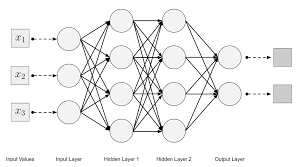
\includegraphics[width=0.6\textwidth]{./plots/DNNArchitecture.png}
  \caption{Diagram of a general architecture of a DNN. Credit image: O'Reilly.~\cite{OReilly}.}
  \label{fig:DNN}
\end{figure}

\ \\The \emph{Universal Approximation Theorem} states that a neural network with one \emph{hidden layer} can in principle approximate any N-dimensional function to an arbitrary degree of accuracy, given a sufficiently large (though finite) number of nodes. In practice however it is more suitable to use multiple hidden layers connected in series~\cite{AndrewNg}.

\ \\In a fully connected NN, each node takes a weighted linear combination of the outputs from nodes of the previous layer, adds its own bias value, and applies an \emph{activation function}, then outputs the result to the neurons of the next layer, as illustrated in Figure~\ref{fig:Neuron}. The activation function is choosen via optimisation for each neuron when the architecture of the NN is defined. 

\begin{figure}[h]
  \centering
  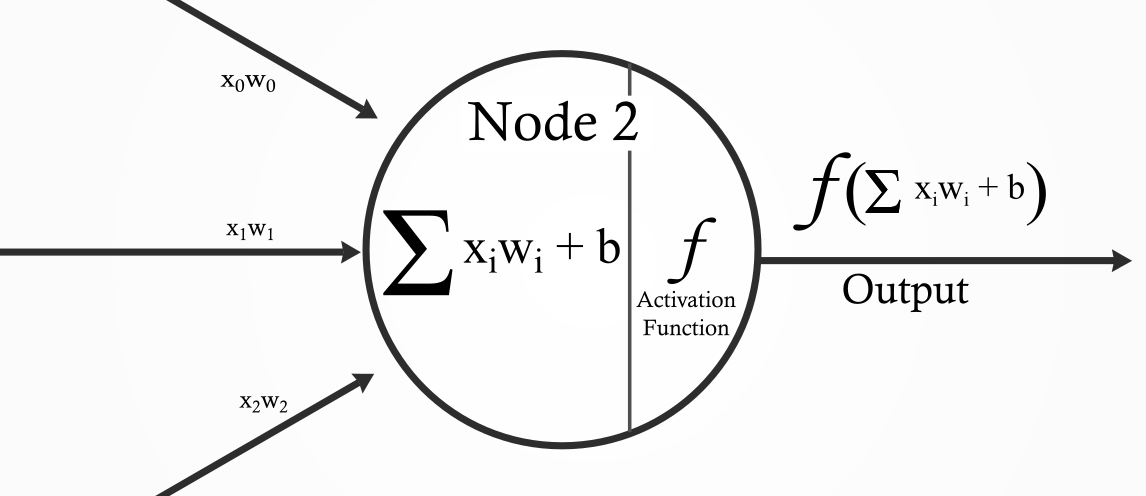
\includegraphics[width=0.6\textwidth]{./plots/Neuron.png}
  \caption{Diagram of a neuron or node in a NN, with its weight inputs, its bias and the output via the activation function. Credit image: The Fork~\cite{TheFork}.}
  \label{fig:Neuron}
\end{figure}

\ \\Once the NN architecture is set, the layers, nodes and activation functions, the total function of the NN is parametrized by all the weights for the connections between nodes plus the biases of each node. Training the NN means learning these weights and biasis so that the NN function can predict well the output when a new data not seen before is taken as input.

\section{Hyper-Parameters}
\label{sec:Hyperparameters}

Several hyper-parameter choices can be made depending on the question being asked, regarding the number of hidden layers, number of nodes on a hidden layer, the activation function of nodes in the hidden layers, the activation function of nodes in the output layer, the learning optimizer, the loss function, the batch size. In the plots of this section the hyper-parameters that are retained for the best performing model are colored in red, to already ilustrate their behaviour relative to the other possible hyper-parameters.

\ \\The problem is a multi-label binary classification. Given a collection (bucket) of 20 hits, for each hit there is a question of a binary classification (if yes or no) the hit belongs to the particle with the largest number of hits in the bucket. 

\ \\The output labels of yes and no may be encoded as 1.0 and 0.0, or as 1.0 and -1.0, respectively. A preliminary study suggests that the latter option provides better results. With this choice, there remains only a limited choice of activation functions of the output layer and of loss functions. 

\ \\Firstly, the output value of the NN prediction fixes the choice of the activation function on the last layer to the hyperbolic tangent (TANH), which has values between -1.0 and 1.0, and not the logistic regression, also called sigmoid, which has values between 0.0 and 1.0, illustrated in Equations

\begin{equation}
   \tanh x = \frac{\sinh x}{\cosh x} = \frac{e^x - e^{-x}}{e^x + e^{-x}} = \frac{e^{2x}-1}{e^{2x}+1}
\end{equation}

\ \\and

\begin{equation}
   S(x) = \frac{1}{1 + e^{-x}} = \frac{e^{x}}{e^{x}+1}.
\end{equation}

\ \\and on the left-hand side of Figure~\ref{fig:ActivationFunctionsLastLayer}. Two more activation functions are possible for values between -1.0 and 1.0. The square non linear (SQNL) is described by Equation

\begin{equation}
   \SQNL~(x) = 
\begin{dcases}
    -1 , & x < -2.0\\
    x + \frac{x^2}{4}, & -2.0 \leq x < 0\\
    x - \frac{x^2}{4}, & 0 \leq x < 2.0\\   
    1 , & x > 2.0\\
\end{dcases}.
\end{equation}

\ \\ and the soft sign (SOSI) function by Equation

\begin{equation}
   \SOSI~(x) = \frac{x}{1 + |x|}.
\end{equation}

\ \\All three functions reach the values of -1.0 and 1.0, but for different values of x. SQNL, TANH and SOSI reach the value of 1.0 (-1.0) for the x values of exactly 2.0 (-2.0), of around $\pi \sim 3.14$ (-$\pi \sim -3.14$) and for $\infty$ ($-\infty$), respectively, as illustarted in the right-hand side of Figure~\ref{fig:ActivationFunctionsLastLayer}.

\begin{figure}[htb]
\centering
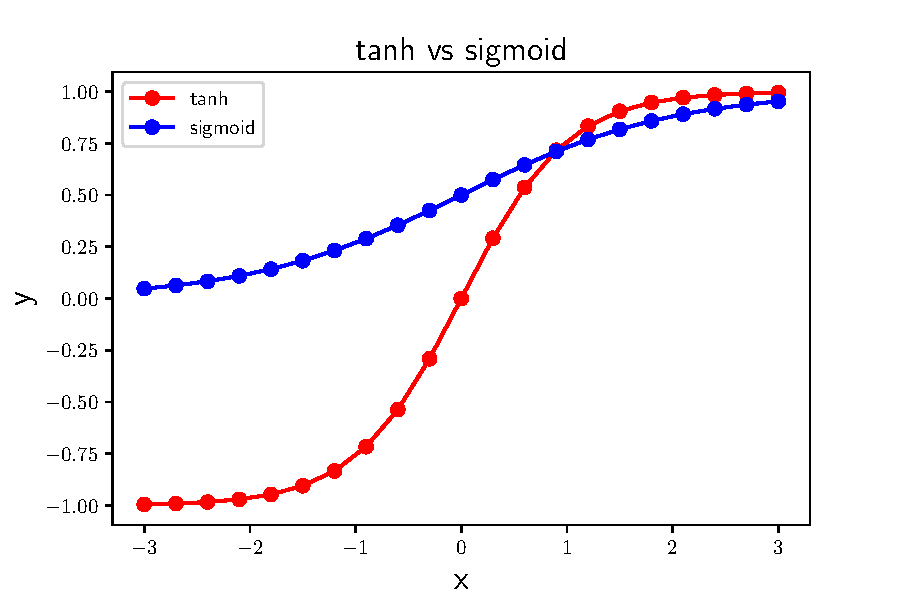
\includegraphics[width=0.45\textwidth]{plots/ActivationFunctionsLastLayer1.pdf}
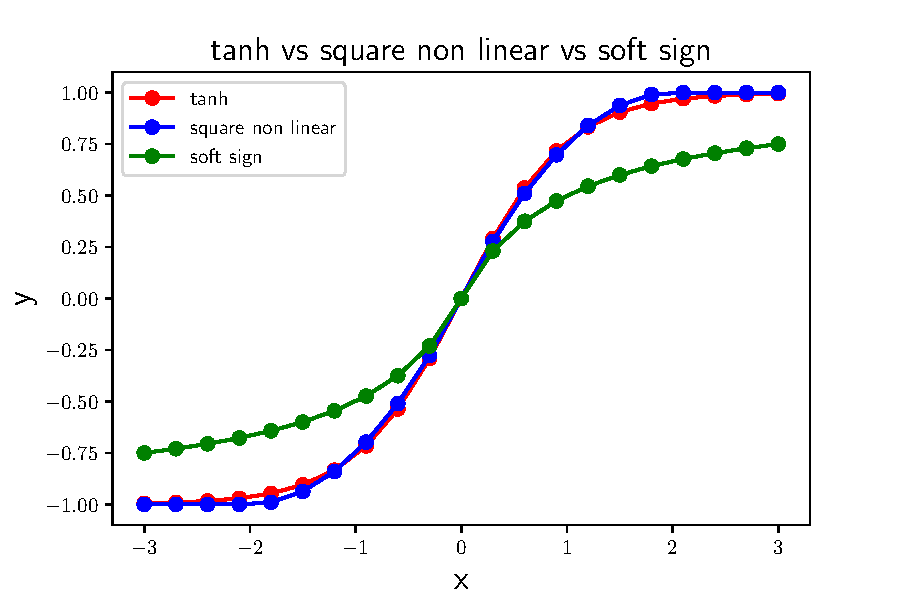
\includegraphics[width=0.45\textwidth]{plots/ActivationFunctionsLastLayer2.pdf}
\caption{Overlaid potential activation functions for the last layer. Left: hyperbolic tangent (tanh) and logistic regression (sigmoid). Right: tanh, square non linear and soft sign. Tanh is chosen as our output labels are -1.0 and 1.0.}
\label{fig:ActivationFunctionsLastLayer}
\end{figure}

\ \\The appropriate loss functions for the target values of -1.0 and 1.0 are only the (regular) hinge function and the squared hinge function. Denoting y the predicted output and t the true target output (label), the hinge function is given by the Equation

\begin{equation}
   \LossFunctionHinge:~l(y) =  \max(0, 1 - t \cdot y),
\end{equation}

\ \\and the squared hinge by the Equation

\begin{equation}
   \LossFunctionSquaredHinge:~l(y) = [\max(0, 1 - t \cdot y)]^2.
\end{equation}

\ \\Their relative behaviour is illustrated in Figure~\ref{fig:LossFunctions} for t=-1.0 (left) and t=1.0 (right). These loss functions never become negative. For t=1.0, for $y \ge t$, the loss function is exactly zero. For $y<t$, the loss function gradually increases. The squared hinge does not have a discontinuity at $y=1$ and at high values increases more than the regular hinge, penalizing large deviations more. The same is valid for y=-1.0, but in the opposite direction. 

\begin{figure}[htb]
\centering
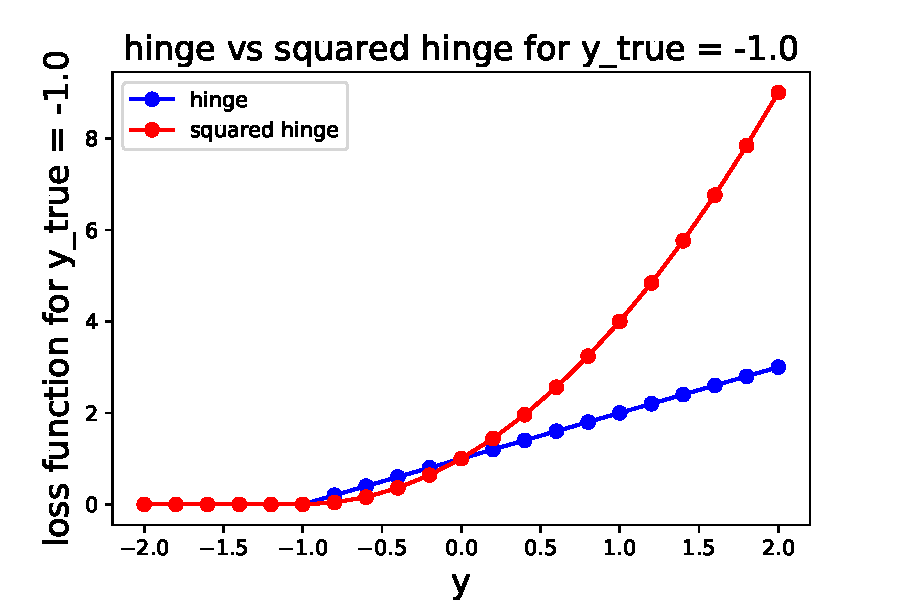
\includegraphics[width=0.45\textwidth]{plots/LossFunctions_MinusOne.pdf}
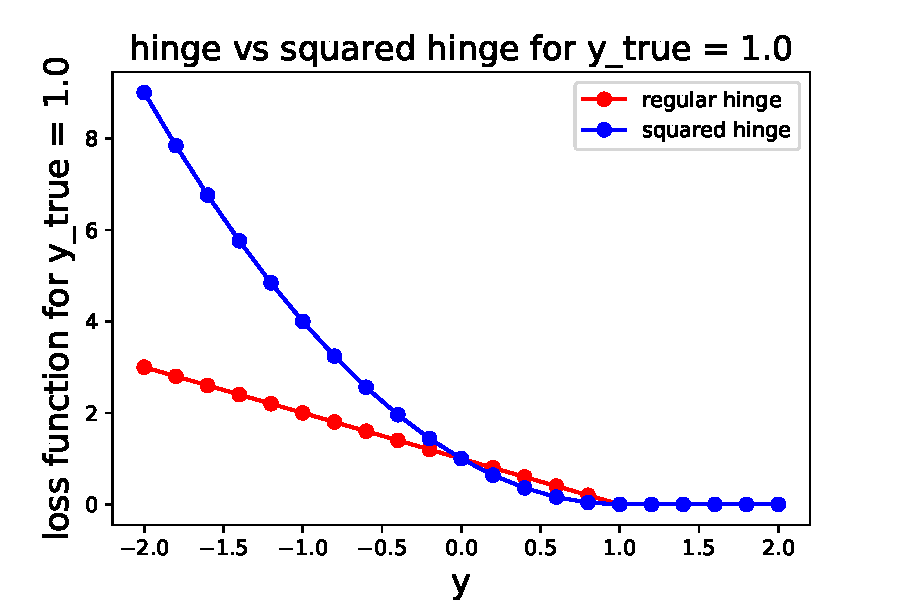
\includegraphics[width=0.45\textwidth]{plots/LossFunctions_PlusOne.pdf}
\caption{Overlaid loss functions of (regular) hinge and squared hinge for varying predicted y, for a fixed true y of -1.0 (left) and 1.0 (right).}
\label{fig:LossFunctions}
\end{figure}

\ \\The functions above apply to a pair of predicted y and true t values. In our problem it refers to each hit. The final loss function for the entire sample represents a sum over all the buckets in all events in the train or test sample, and for each bucket the sum over each of the 20 hits, as exemplified in Equation

\begin{equation}
   \LossFunctionHinge:~l(y) = \sum_{\rm bucket} \sum_{\rm hit} \max(0, 1 - t_{\rm hit} \cdot y_{\rm hit})
\end{equation}

\ \\ and

\begin{equation}
   \LossFunctionSquaredHinge:~l(y) = \sum_{\rm bucket} \sum_{\rm hit} [\max(0, 1 - t_{\rm hit} \cdot y_{\rm hit})]^2.
\end{equation}

\ \\Another choice to make is that of the activation functions for the nodes of the hidden layers. Besides the already-mentioned sigmoid and hyperbolic tangent functions, the Rectified Linear Unit (ReLU) is introduced. ReLU is the mostly common activation function for neural networks nowadays, including for more advanced neural networks such as convolutional neural networks (CNN) or deep neural networks (DNN). ReLU is \emph{rectified} from the bottom, meaning its values are zero for negative inputs and return the same value as the input for positive inputs. ReLU can be summarized by Equation

\begin{equation}
   \ReLU:~R(x)= \max(0, x).
\end{equation}

\ \\While both the function R(x) and its derivative are monotonous, the function also has some drawbacks. is not differentiable at zero. Since for all negative values the input is exactly zero, for methods learning with gradient descent, the ability to learn is reduced. To address this problem, a variation of ReLU is introduced, namely and the Exponential Linear Function (ELU), described by Equation

\begin{equation}
     \ELU:~E(x= 
\begin{dcases}
    \alpha(e^x -1), & x < 0\\
    x,              & x \geq 0
\end{dcases}.
\end{equation}

\ \\For positive values, the function remains the same. But for the negative values, an exponential curve appears, tending smoothly to a constant value $\alpha$. ELU has the advantage over ReLU to be fully continuous and differentiable, and not having a vanishing gradient problem for gradient descent learning. Its main disadvtange is that it is slower to compute for negative values. But it may be worth it for a more precise result. The comparison of the ReLU and ELU functions is illustrated in Figure~\ref{fig:ActivationFunctionsHiddenLayers}.

\begin{figure}[htb]
\centering
\includegraphics[width=0.45\textwidth]{plots/ActivationFunctionsHiddenLayers.pdf}
\caption{Overlaid activation functions of ReLU and ELU, with $\alpha=1.0$.}
\label{fig:ActivationFunctionsHiddenLayers}
\end{figure}

\ \\Another hyper-parameter to tune is the number of hidden layers and the number of nodes on each hidden layer. The \emph{Universal Approximation Theorem} suggests that one layer with a very large number of nodes is enough to learn any arbitrary function. But in practice it is worth having several consecutive layers of fewer nodes per layer. That forms a deep neural network. 

\ \\Another option in the architecture of the NN is whether to use or not to add a regularisation layer, in particular a dropout layer~\cite{DropoutLayer}. Sometimes the resulting model is too complex relative to the quantity of input data, leading to overfitting during training. Overfitting is similar to memorisation of the input data, leading to not be able to predict correctly on new data. To avoid overfitting, regularisation techniques are used. Typical methods add a new term to the loss functions. Other techniques add a dropout layer. The dropout method sets randomly some of the inputs to 0 with a frequency $f$, and reweights the other inputs by $1/(1-f)$, so that the total sum of inputs remains constant. The value of $f$ is a hyper-parameter to be optimised. The location of the dropout layer is usually between the hidden layers and the last layer. Dropout is applied only during training, and not during testing or infering on new data.

\ \\Another choice related to the learning method is the learning optimiser. Two algorithms based on stochastic gradient descent are compared, namely Adam~\cite{Adam} and AdaDelta~\cite{AdaDelta}. For both their default parameters are used, the most important being the learning rate of 0.001. Adam is very computationally efficient, while AdaDelta uses adaptive learning rate. 

\section{Learning Methods}

NN training is done learning on the training dataset and testing on the testing dataset. Running once over all the data from training and testing represents an \emph{epoch}. During an epoch, events are analysed in groups called \emph{batches}. The number of epochs to run on and the number of events in each batch can be optimised.

\ \\ Let's take a look at how the NN training happens. At first the NN has random values for the weights and biases. For each of the events in the first batch, data comes in, and the NN predicts an output values, that are at first very different from the true desired output value. To evaluate how far away are the predicted output from the desired output, a \emph{loss} function is defined that can be chosen from several formulas, but have the generic form of a sum over the absolute values of these differences. The goal of the NN training is to update the values of the weights and biases so that the loss function is minimized. After the first batch, the NN changes the weights via a back-propagation aglorithm using the optimiser algorithm. For each new batch, the weights and biases change, and become continously closer to the correct values, as the loss function becomes gradually smaller. When all the training events are used, the first epoch is finished. The NN function at this point is then applied to the new dataset from the testing dataset, which is not split in batches, and a loss function is also calculated. The entire procedure repeats for the number of epochs chosen. At the end, the final weights and biases define the final NN model that has been learned.

\section{Train and Test Split and k-fold}
\label{sec:TrainAndTest}

The k-fold validation is a procedure used to test the effectiveness of a machine learning model. It is used especially if the data are limited. Normally, the data are split in two equal parts (train and test), corresponding to k=2. For a general k, the data are split randomly into k groups. k-1 groups are used in training and the last one in testing. The operation is repeated by permuting the groups, so that each group is used only once in testing. The final result is obtained by averaging out the permutations.

\ \\It is also possible to split into two unequal parts. In this project the split is done with k=2, 70\% in train and 30\% in test. Although teach data sample is a bucket, it is convenient to use that events have about the same number of buckets. The split of 100 events is done with 70\% of events in train and 30\% of events in test. One can split the events randomly, as by the laws of particle physics events simulate independent particle collisions. NN training takes a significant amount of time. It is useful to train on an increasing data sample size and check if the performance reaches a plateau. For convenience, to study easily with a step of 10 events, events are grouped in consecutive order by 10, with the first 7 events being used for training (Train sample) and the following 3 events are used for testing (Test sample). The pseudo-code is described in Appendix~\ref{sec:AppendixPseudoCodeInputOutput}.

\section{Balancing Datasets}
\label{sec:BalancingDatasets}

It is common practice in ML classification problems that the signal target is much rarer than the backgrounds. It is said the dataset is unbalanced. The solution is to balance the dataset by increasing the weights of signal events such that the total sum of weights of signal equals the total sum of weights for background. The NN learning uses for each data samples its own specific weight. A balanced dataset is used for training. It is not used in testing, in order to represent a real-world situation when one tries to predict the proportion of signa to background, and does not know the balancing ratio. 

\ \\This project involves a multi-label classification problem, where there are 20 hits in a bucket, and for each hit a classification question is asked, if it is a signal (1) or background (0) relative to being part of the majority particle in the bucktet. From physics studies in Chapter~\ref{chapter:TrackML}, it is decided that all buckets with less than 10 hits with output = 1, have all their hits set to output = -1. The dataset becomes even more unbalanced. Balancing is done in two steps.

\ \\First, buckets are removed so that there are equal number of buckets for each of \nbPositiveHit\ between 10 and 17. Values 18-20 are left unchanged, as they are too small. The goal is to learn uniformly and not be biased towards a particular category. \nbPositiveHit~between 1 and 9 are zero by constructions, as all these values are moved to \nbPositiveHit~of zero, which originally did not have any entries. Then the number of buckets of \nbPositiveHit=0 is reduced so that overall, there are exactly equal numbers of positive and negative hits in the sample. That ensures the most general way for learning, without a bias towards one category or the other. The training set is balanced, keeping about 130k buckets. The testing set remains unbalanced, with roughly 3.2M bckets.

\section{Hyper-Parameter Tuning}
\label{sec:HyperparameterTuning}

The hyper-parameters are tuned by choosing the models that perform best in the test sample over 300 epochs, looking at the accuracy and loss that result directly from Keras/TensorFlow after the training. In the plots of this section, the best model summarised in Section~\ref{sec:BestModel} is compared with alternative models where all hyper-parameters are kept constant, except one that is changed. Since training on 1200 epochs and an unbalanced test dataset takes too long, 300 epochs and the balanced test dataset are used. The balanced train dataset are used both in this study and for the final result with 1200 epochs, described in Chapter~\ref{chapter:ModelPerformance}. From this study the best performining hyper-parameters are chosen. When the performance of several hyper-parameters is similar, the simplest or most commonly used hyper-parameter is chosen. The resulting final model is presented in Section~\ref{sec:BestModel}.

\subsection{DNN Architecture}
\label{sec:DNNArchitecture}

A comparison of the number of hidden layers is studied. The performance is similar for different values, and 3 hidden layers is retained for the final model, as it provides a slightly better performance, as illustrated in Figure~\ref{fig:HPNbHiddenLayers}.

\begin{figure}[htb]
\centering
\includegraphics[width=0.32\textwidth]{plots/plot_01_1_overlay_graph_accuracyBinary_Train_NbHiddenLayers.pdf}
\includegraphics[width=0.32\textwidth]{plots/plot_01_1_overlay_graph_accuracyBinary_Test_NbHiddenLayers.pdf}\\
\includegraphics[width=0.32\textwidth]{plots/plot_01_1_overlay_graph_loss_Train_NbHiddenLayers.pdf}
\includegraphics[width=0.32\textwidth]{plots/plot_01_1_overlay_graph_loss_Test_NbHiddenLayers.pdf}\\
\caption{Comparison of different numbers of hidden layers. 3 hidden layer is best. Binary accuracy and loss in Train and Test balanced samples.}
\label{fig:HPNbHiddenLayers}
\end{figure}

\ \\A comparison of the number of nodes on the hidden layers is studied. For simplicity, in this study it is considered the same number of nodes on each hidden layer. The performance is similar for different values, and 200 nodes on the hidden layers is retained for the final model, as illustrated in Figure~\ref{fig:HPNbNodesOnHiddenLayers}. This represents 10 times more than the nodes on the output layer.

\begin{figure}[!htb]
\centering
\includegraphics[width=0.32\textwidth]{plots/plot_01_1_overlay_graph_accuracyBinary_Train_NbNodesOnHiddenLayers.pdf}
\includegraphics[width=0.32\textwidth]{plots/plot_01_1_overlay_graph_accuracyBinary_Test_NbNodesOnHiddenLayers.pdf}\\
\includegraphics[width=0.32\textwidth]{plots/plot_01_1_overlay_graph_loss_Train_NbNodesOnHiddenLayers.pdf}
\includegraphics[width=0.32\textwidth]{plots/plot_01_1_overlay_graph_loss_Test_NbNodesOnHiddenLayers.pdf}\\
\caption{Comparison of the ratio of the different number of nodes on the hidden layers divided by the number of nodes on the last layer. k=10, or 200 nodes on each hidden layer, is best. Binary accuracy and loss in Train and Test balanced samples.}
\label{fig:HPNbNodesOnHiddenLayers}
\end{figure}

\ \\A comparison of the activation functions for the hidden layers, namely ReLU and ELU, is performed. For simplicity, in this study it is considered that all nodes of all hidden layers have the same activation function. The performance is similar between the two options, so the standard and mostly used ReLU is retained for the final model, as illustrated in Figure~\ref{fig:HPActivationFunctionHiddenLayers}.

\begin{figure}[!htb]
\centering
\includegraphics[width=0.32\textwidth]{plots/plot_01_1_overlay_graph_accuracyBinary_Train_ActivationFunctionHiddenLayers.pdf}
\includegraphics[width=0.32\textwidth]{plots/plot_01_1_overlay_graph_accuracyBinary_Test_ActivationFunctionHiddenLayers.pdf}\\
\includegraphics[width=0.32\textwidth]{plots/plot_01_1_overlay_graph_loss_Train_ActivationFunctionHiddenLayers.pdf}
\includegraphics[width=0.32\textwidth]{plots/plot_01_1_overlay_graph_loss_Test_ActivationFunctionHiddenLayers.pdf}\\
\caption{Comparison of ReLU and ELU activation functions on the hidden layers. ReLU is chosen for the final model. Binary accuracy and loss in Train and Test balanced samples.}
\label{fig:HPActivationFunctionHiddenLayers}
\end{figure}

\ \\A comparison of adding or not adding a regularisation function via the dropout layer at the end of the hidden layers is studied. The performance is better by having a dropout layer, as illustrated in Figure~\ref{fig:HPDropoutLayer}.

\begin{figure}[!htb]
\centering
\includegraphics[width=0.32\textwidth]{plots/plot_01_1_overlay_graph_accuracyBinary_Train_DropoutLayer.pdf}
\includegraphics[width=0.32\textwidth]{plots/plot_01_1_overlay_graph_accuracyBinary_Test_DropoutLayer.pdf}\\
\includegraphics[width=0.32\textwidth]{plots/plot_01_1_overlay_graph_loss_Train_DropoutLayer.pdf}
\includegraphics[width=0.32\textwidth]{plots/plot_01_1_overlay_graph_loss_Test_DropoutLayer.pdf}\\
\caption{Comparison without and with a dropout layer for regularisation. A dropout layer is used in the final model. Binary accuracy and loss in Train and Test balanced samples.}
\label{fig:HPDropoutLayer}
\end{figure}

\ \\A comparison of the activation functions for the last layer, namely TANH, SQNL and SOSI, is studied. The performance is similar for the three options, so the standard and mostly used TANH is retained for the final model, as illustrated in Figure~\ref{fig:HPActivationFunctionLastLayer}.

\begin{figure}[!htb]
\centering
\includegraphics[width=0.32\textwidth]{plots/plot_01_1_overlay_graph_accuracyBinary_Train_ActivationFunctionLastLayer.pdf}
\includegraphics[width=0.32\textwidth]{plots/plot_01_1_overlay_graph_accuracyBinary_Test_ActivationFunctionLastLayer.pdf}\\
\includegraphics[width=0.32\textwidth]{plots/plot_01_1_overlay_graph_loss_Train_ActivationFunctionLastLayer.pdf}
\includegraphics[width=0.32\textwidth]{plots/plot_01_1_overlay_graph_loss_Test_ActivationFunctionLastLayer.pdf}\\
\caption{Comparison of TANH, SQNL and SOSI as activation functions on the last layer. TANH is used in the final model. Binary accuracy and loss in Train and Test balanced samples.}
\label{fig:HPActivationFunctionLastLayer}
\end{figure}

\subsection{DNN Learning}
\label{sec:DNNLearning}

Moving on from the hyper-parameters that define the geometry of the deep neural network to those defining its learning method, a comparison of the optimizers, Adam and AdaDelta, each with its default parameters, is studied. The performance of Adam is significantly better than that of AdaDelta, so Adam is retained for the final model, as illustrated in Figure~\ref{fig:HPOptimizer}.

\begin{figure}[!htb]
\centering
\includegraphics[width=0.32\textwidth]{plots/plot_01_1_overlay_graph_accuracyBinary_Train_Optimizer.pdf}
\includegraphics[width=0.32\textwidth]{plots/plot_01_1_overlay_graph_accuracyBinary_Test_Optimizer.pdf}\\
\includegraphics[width=0.32\textwidth]{plots/plot_01_1_overlay_graph_loss_Train_Optimizer.pdf}
\includegraphics[width=0.32\textwidth]{plots/plot_01_1_overlay_graph_loss_Test_Optimizer.pdf}\\
\caption{Comparison of Adam and AdaDelta optimizers for the learning method. Adam is used in the final model. Binary accuracy and loss in Train and Test balanced samples.}
\label{fig:HPOptimizer}
\end{figure}

\ \\A comparison of the loss functions used to learn the weights and biases of the DNN via gradient descent, regular hinge and squared hinge, is studied. Their performance is similar, so the standard and mostly used regular hinge is retained for the final model, as illustrated in Figure~\ref{fig:HPLossFunction}.

\begin{figure}[!htb]
\centering
\includegraphics[width=0.32\textwidth]{plots/plot_01_1_overlay_graph_accuracyBinary_Train_LossFunction.pdf}
\includegraphics[width=0.32\textwidth]{plots/plot_01_1_overlay_graph_accuracyBinary_Test_LossFunction.pdf}\\
\includegraphics[width=0.32\textwidth]{plots/plot_01_1_overlay_graph_loss_Train_LossFunction.pdf}
\includegraphics[width=0.32\textwidth]{plots/plot_01_1_overlay_graph_loss_Test_LossFunction.pdf}\\
\caption{Comparison of regular and square hinge loss functions for DNN learning. Regular hinge is used in the final model. Binary accuracy and loss in Train and Test balanced samples.}
\label{fig:HPLossFunction}
\end{figure}

\ \\The conclusion is that the learning part of the hyper-parameters tuning by comparing various batch sizes. The best performance is obtained for 50000, which is retained for the final model, as illustrated in Figure~\ref{fig:HPBatchSize}.

\begin{figure}[!htb]
\centering
\includegraphics[width=0.32\textwidth]{plots/plot_01_1_overlay_graph_accuracyBinary_Train_BatchSize.pdf}
\includegraphics[width=0.32\textwidth]{plots/plot_01_1_overlay_graph_accuracyBinary_Test_BatchSize.pdf}\\
\includegraphics[width=0.32\textwidth]{plots/plot_01_1_overlay_graph_loss_Train_BatchSize.pdf}
\includegraphics[width=0.32\textwidth]{plots/plot_01_1_overlay_graph_loss_Test_BatchSize.pdf}\\
\caption{Comparison of various batch sizes for DNN learning. A batch size of 50000 is used in the final model. Binary accuracy and loss in Train and Test balanced samples.}
\label{fig:HPBatchSize}
\end{figure}

\subsection{Best Model}
\label{sec:BestModel}

The problem structure fixes the number of nodes on the input layer to 60 (3 coordinates for 20 hits), and of the output layer to 20 (1 boolean for 20 hits). The DNN architecture and learning methods are optimised as hyper-parameters, whose options are limited by the choice of representing the answers yes and no by 1.0 and -1.0, respectively. The hyper-parameters that describe the best model are summarised as follows.

\ \\There are 3 hidden layers, each with 200 nodes, or 10 times more than the number of nodes in the output layer. A reminder is that the input layer has 60 nodes (3 coordinates x, y, z for each of the 20 hits in the bucket) and the output layer has 20 nodes (an output of -1.0 or 1.0 for each of the 20 hits in the bucket). A dropout layer (0.2) is added at the end of the hidden layers. The activation function for the hidden layers is the rectified linear unit (ReLU). The activation function for the last layer is hyperbolic tangent ($\tanh$). The loss function is the (regular) hinge function. The batch size is 50000.

\ \\While the choice of hyper-parameters is done using 300 epochs and the balanced test dataset, the final result uses 1200 epochs and the unbalanced test dataset.

\section{Predicting or Inference and Figures of Merit}

Once the model is trained, it can be applied to a new dataset to infer or make a prediction.

\ \\Besides the value of the loss function across the entire dataset, there is also another figure of merit of how well does a NN perform in training and testing. It is called \emph{accuracy} and is related to the number of of true positives or false negatives. The larger the accuracy, the better.

\ \\For the training dataset, the loss and accuracy values always improve. But in the testing dataset they can start to degrade if we train for too many epochs. By degrading it means that the loss value starts to grow, and the accuracy value starts to decrease. That is called over-training and consists of memorizing the inputs, and thus not being able to predict correctly any more for new inputs.

\ \\The confusion matrix is a table that summarises the performance of a binary classification model, as illustrated in Table~\ref{tab:ConfusionMatrix}. 

\begin{table}[h!]
 \centering
   
    \begin{tabular}{|l|l|} % <-- Alignments: 1st column left, 2nd middle and 3rd right, with vertical lines in between
      \hline
      TP & FP \\
      \hline
      FN & TN \\
      \hline
    \end{tabular}
\caption {Confusion Matrix.}
\label{tab:ConfusionMatrix}
\end{table}

\ \\The four metrics presented in the table are true positive (TP), false positive (FP), false negative (FN), and true negative (TN). Based on these four numbers further figures of merit are derived.

\ \\The accuracy defines what percentage of the total predictions are classified correctly, either as TP or TN, as defined by the Equation

\begin{equation}
   \Accuracy = \frac{\TP + \TN}{\TP + \TN + \FP + \FN}.
\end{equation}

\ \\The precision defines the percentage of the predicted positive that are actually positive, as defined by Equation

\begin{equation}
   \Precision = \frac{\TP}{\TP + \FP}.
\end{equation}

\ \\The recall defines the percentage of actual positive that are correctly predicted, as defined by the Equation

\begin{equation}
   \Recall = \frac{\TP}{\TP + \FN}.
\end{equation}

\ \\ The equivalents of the precision and recall can be constructed also for the negative values, as if the negative values are the sought target. The negative predicted value is the negative equivalent of precision and it represents the percentage of the predicted negative that in reality are also negative, as defined by the Equation

\begin{equation}
   \NegativePredictedValue = \frac{\TN}{\TN + \FN}.
\end{equation}

\ \\The true negative rate is the negative equivalent of the recall. It defines the percentage of the real negative that are also predicted as negative, as defined by the Equation 

\begin{equation}
   \TrueNegativeRate = \frac{\TN}{\TN + \FP}.
\end{equation} 

\ \\The pseudo-code to calculate the metrics is described in Appendix~\ref{sec:AppendixModelEvaluationMetrics}. 

\section{Software Used}

Several software Python libraries are used to perform this study, including data manipulation, the NN training, the figure of merit evaluation and plotting.

\ \\Numpy is a Python programming library, which is a coding support for large multi-dimensional arrays and matrices~\cite{Numpy}. 

\ \\PANDAS is a data manipulation and analysis library~\cite{PANDAS}. It is an open source library that is made mainly for working with relational or labeled data. It provides various data structures and operations for manipulating numerical data and time series. It is fast, has high performance and productivity. Data frames is a two-dimensional data structure with labeled data (rows and columns). Pandas uses numpy behind the hood. 

\ \\Jupyter Notebook is an important tool in the data science field. It is a web-based interactive computing platform~\cite{JupyterNotebook}. The Notebook combines code, equations, text, visualisation, interactive dashboard and other media. It works in line code, using blocks. 

\ \\Matplotlib is used for producing the plots in this thesis, both 1D and 2D~\cite{Matplotlib}.



\chapter{Model Performance}
\label{chapter:ModelPerformance}

In this chapter the performance metrics of the best deep neural network model are described. The hyper-parameters values for the best model are enumerated in Section~\ref{sec:BestModel}.

\section{Training Metrics}
\label{sec:Training}

In Figure~\ref{fig:AccuracyLoss} the binary accuracy and loss function are presented as resulted directly from training in Keras and Tensorflow. Note that while Train is balanced and in general Test is unbalanced, for these plots Test is also balanced. The reason is that it would be too slow to train the NN with 1200 epochs with Test unbalanced. Training is done on the balanced Train dataset. Prediction is done on the unbalanced Test dataset.

\begin{figure}[t]
\centering
\includegraphics[width=0.45\textwidth]{plots/plot_01_1_overlay_graph_accuracyBinary_Train.pdf}
\includegraphics[width=0.45\textwidth]{plots/plot_01_1_overlay_graph_accuracyBinary_Test.pdf}\\
\includegraphics[width=0.45\textwidth]{plots/plot_01_1_overlay_graph_loss_Train.pdf}
\includegraphics[width=0.45\textwidth]{plots/plot_01_1_overlay_graph_loss_Test.pdf}\\
\caption{Binary accuracy and loss, as resulted directly from training in Keras and Tensorflow. Note that while Train is balanced, Test is also balanced, as it would be too slow to have it unbalanced.}
\label{fig:AccuracyLoss}
\end{figure}

\section{Hit-Level Metrics}
\label{sec:HitLevelMetrics}

In this section the metrics at the hit-level are studied. A bucket is made of 20 hits. Figure~\ref{fig:OutputOutputPredicted1D} presents at the top the distribution of the number of positive hits ($\nbPositiveHit$), at the bottom the distribution of the number of hits predicted to be positive, with Train on the left and Test on the right. The distributions are normalised, so their shapes can be compared. The number of events used in Train relative to Test is 7 to 3. Furthermore, the Train dataset is balanced, keeping only a tiny subset of the buckets, while the Test dataset is unbalanced, keeping all of its buckets. In both datasets all values of $\nbPositiveHit < 10$ are set artificially to 0, considering there was no hit belonging to an interesting particle. Furthermore, the Train dataset is balanced, so that buckets with $\nbPositiveHit$ between 10 and 17 are eliminated, so that equal numbers of buckets for each \nbPositiveHit~remain. Since the distribution is falling (as seen in the Test plot), all values take the lower value of the bin 17. Values 18-20 are left unchanged, as they are too small. Values 18-20 are left unchanged, as they are too small.

\ \\Tests were done with values varying from 14 to 20, but 17 had by far the best outcome. Lower than 17 would not have a training distribution flat enough. Higher than 17 would leave very few buckets to train on. 

\ \\At the bottom of Figure~\ref{fig:OutputOutputPredicted1D} there are the equivalent plots after the prediction using our model. The training is quite solid. There is a tall bin at $\nbPositiveHit=0$, followed by virtually empty bins, and the distributions starts to grow at $\nbPositiveHit=10$, just as in the desired output distribution. For the higher bins, the relative shape does not agree fully to the desired output. For Train, instead of being flat, the distribution increases with larger \nbPositiveHit. For Test it decreases as expected, but not nearly as fast. Overall, however, the model behaves quite well, relative to many other hyper-parameter settings tried.


\begin{figure}[t]
\centering
\includegraphics[width=0.45\textwidth]{plots/plot_02_1_overlay_histo_OutputPositive_Train.pdf}
\includegraphics[width=0.45\textwidth]{plots/plot_02_1_overlay_histo_OutputPositive_Test.pdf}\\
\includegraphics[width=0.45\textwidth]{plots/plot_02_1_overlay_histo_PredictedOutputPositive_Train.pdf}
\includegraphics[width=0.45\textwidth]{plots/plot_02_1_overlay_histo_PredictedOutputPositive_Test.pdf}\\
\caption{Output and output predicted 1D. Older ones have a sharp peak, the new ones are more flat.}
\label{fig:OutputOutputPredicted1D}
\end{figure}

\ \\Figure~\ref{fig:OutputOutputPredicted2D} presents the 2D distributions of the output predicted vs output in terms of number of positive hits. The color coding is proportional to the number of entries in the 2D histogram. As expected, there is a peak at (0, 0), meaning events with exactly zero number of positive hits (after the move of all values smaller than 10 to 0), and that are also predicted to have exactly zero. There is nothing between 1 and 9. And for values $\ge 10$, there is a diagonal, as expected for the Train balanced. For the Test unbalanced, it is harder to see. But indeed most entries are in the top left corner of this region, as expected.


\begin{figure}[t]
\centering
\includegraphics[width=0.45\textwidth]{plots/plot_04_1_overlay_histo2D_OutputPositive_PredictedOutputPositive_03_10_R_RH_B_1200_Train.pdf}
\includegraphics[width=0.45\textwidth]{plots/plot_04_1_overlay_histo2D_OutputPositive_PredictedOutputPositive_03_10_R_RH_B_1200_Test.pdf}\\
\caption{Output and output predicted 2D. In Train balanced, a diagonal is seen. In Test unbalanced it's harder to see.}
\label{fig:OutputOutputPredicted2D}
\end{figure}

\ \\From these plots it can be concluded that in the balanced dataset (Train and Test) a diagonal can be nicely seen. In the Test unbalanced it is harder to see, but still values look relatively flat in 1D. 

\ \\Figure~\ref{fig:FiguresOfMerit1} presents figures of merit at hit level for each \volumeID~in the detector. By looping over all buckets and all hits, both the true and predicted output labels for each hit are known. It results if the hit is TP (True Positive), FP (False Positive), FN (False Negative), or TN (True Negative). The number of hits in these four categories in each \volumeID~is counted. From these for each \volumeID~there are estimated the figures of merit of accuracy, precision, recall, predicted output negative and true negative rate. They all need to be as high as possible, ideally 1. As it is impossible for one model to satisfy all criteria, as known from the bias-variance trade-off, a model with overall good performance across all categories is chosen.

\begin{figure}[t]
\centering
\includegraphics[width=0.45\textwidth]{plots/plot_03_1_overlay_graph_Accuracy_VolumeID_Train.pdf}
\includegraphics[width=0.45\textwidth]{plots/plot_03_1_overlay_graph_Accuracy_VolumeID_Test.pdf}\\
\includegraphics[width=0.45\textwidth]{plots/plot_03_1_overlay_graph_Precision_VolumeID_Train.pdf}
\includegraphics[width=0.45\textwidth]{plots/plot_03_1_overlay_graph_Precision_VolumeID_Test.pdf}\\
\includegraphics[width=0.45\textwidth]{plots/plot_03_1_overlay_graph_Recall_VolumeID_Train.pdf}
\includegraphics[width=0.45\textwidth]{plots/plot_03_1_overlay_graph_Recall_VolumeID_Test.pdf}\\
\includegraphics[width=0.45\textwidth]{plots/plot_03_1_overlay_graph_PredictedOutputNegative_VolumeID_Train.pdf}
\includegraphics[width=0.45\textwidth]{plots/plot_03_1_overlay_graph_PredictedOutputNegative_VolumeID_Test.pdf}\\
\includegraphics[width=0.45\textwidth]{plots/plot_03_1_overlay_graph_TrueNegativeRate_VolumeID_Train.pdf}
\includegraphics[width=0.45\textwidth]{plots/plot_03_1_overlay_graph_TrueNegativeRate_VolumeID_Test.pdf}\\
\caption{Accuracy, precision, recall, predicted output negative, true negative rate. Train (left) and Test (right). }
\label{fig:FiguresOfMerit1}
\end{figure}


\section{Particle-Level Metrics}
\label{sec:ParticleLevelMetrics}

Two numpy arrays of dimension two are used: the true output and the output predicted by the model. Each row represents a bucket. There are 20 columns, representing the 20 hits. A for loop over buckets is made. For each bucket a loop over hits is made. Each hit has a value of -1 or +1 for the output and for the predicted output. For the current bucket, the number of hits that are positive (\nbPositiveHit) is counted. A count is also made for those that are both positive and in addition predicted to also be positive (\nbTruePositiveHit). A bucket with $\nbPositiveHit \ge10$ is considered to contain a truth particle. If in addition the bucket has also $\nbTruePositiveHit /\nbPositiveHit > 80\%$, it is considered to also have reconstructed correctly that particle. A count is made of the buckets that have a truth particle, and then those that both have a truth particle and have reconstructed it. The efficiency to reconstruct a particle ($\eff = \nbParticleReco / \nbParticleTruth$) is 84.2\% for Train and 71.3\% for Test. Detailed results are summarized in Table~\ref{tab:ParticleReconstructionEfficiency}.

\begin{table}[h!]
\centering
  \resizebox{\textwidth}{!}{
    \begin{tabular}{|l|l|l|l|l|} % <-- Alignments: 1st column left, 2nd middle and 3rd right, with vertical lines in between
      \hline
      Sample & \eff & \nbBucket & \nbParticleTruth & \nbParticleReco \\
      \hline
      Train Balanced & 84.2\% & 130k &  94k & 79k \\
      Test Balanced & 74.9\%  & 62k & 45k & 34k \\
      Test Unbalanced & 71.3\% & 3219k & 1178k & 840k \\
      \hline
    \end{tabular}
  }
\caption {Particle reconstruction efficiency results.}
\label{tab:ParticleReconstructionEfficiency}
\end{table}

\chapter{Conclusions}
\label{Conclusions}

\section{Conclusions}

CERN experiments at the LHC plan to continue their studies of the building blocks of the Universe by studying proton-proton collisions with ever instantaneous luminosity. This improves the probability that interesting particles are produced, such as the Higgs boson, top quarks, W and Z bosons, and hopefully also particles predicted by models Beyond the Standard Model. It translates to increasing number of collisions per bunch crossing (pile-up $\mu$). For Run-4, $\mu$ is expected to reach a value of 200, from a maximum around 60 today. The drawback is that the particle events become much busier, with many more particles overlapping. Reconstructiong these particles becomes harder. So much so that computing resources are predicted to not be enough to reconstruct Run-4 detector data and simulation data. 

\ \\The solution is to improve dramatically particle reconstruction from the algorithm and software side. In this regard, machine learning is a promising avenue studied thorougly at CERN. In this thesis, a deep neural network (DNN) is studied to reconstruct particles from hit data in the inner detector, using simulations of a general particle physics detector at CERN, provided by the TrackML data challenge. The inner detector is split into subdetectors and regions defined by the \volumeID, \layerID~and \moduleID. For each simulated hit, both the reconstructed position and the original (true) position is known. Also the \particleID~of the particle producing the hit is known. This allows to build a supervised machine learning algorithm, to study groups of hits at a time and try to identify the particle with the largest number of hits in the group. First all hits in an event are organised in an approximate nearest neighbour tree based on their spatial position. For each hit in the detector a group of hits is created consisting of hits that are closest to the direction of the line that connects this hit with the original collision in the center of the detector. Such group is denoted a bucket. Since a particle leaves typically around 10 hits in the detector, the bucket size is chosen to be 20. However,the number of hits belonging to the particle with the largest number of hits is counted. If this number is smaller than 10, then it is considered that none of the hits belongs to this particle, and the labels of all hits are reset to -1. The goal is therefore that in each group of 20 hits, to identify those that belong to a particle that has at least 10 hits. It is a multi-class binary classificiation problem, as for each hit in the bucket there is a question that can be answered by yes or no, namely if the hit belongs to the particle with the largest number of hits in the bucket. 

\ \\A deep neural network algorithm is trained, using Keras and TensorFlow in Python. 100 events are used, split 70\% in training and 30\% in testing. The training data set is balanced. The test sample is studied both in a balanced and unbalanced format The balanced training set has about 130k buckets, the balanced testing set about 62k buckets, and the unbalanced testing seet about 3.2M buckets. Hyper-parameters are tuned and the resulting structure of the best model is summarised in Section~\ref{sec:BestModel}.

\ \\The final performance metrics are shown for the unbalanced dataset, ensuring a particle reconstruction efficiency of 71.3\%. 

\section{Future Plans}

Given more time, several improvements or new studies may enhance the current results.

\ \\The output labels of the hits of no and yes are represented by -1.0 and 1.0. One can represent them also as 0.0 and 1.0. This leads to the use of other activation functions on the last layer and to other loss functions. A preliminary study suggests that -1.0/1.0 behave better than 0.0/1.0, but a more thorough study may be performed. 

\ \\Only 100 events have been studied in this project. The entire TrackML dataset is 100 times larger, consisting of 10000 events. Deep learning methods benefit from using large quantities of data. Using the entire dataset should provide a better peforming model. The technical challenges will remain the computing power needed for training. Dedicated resources at CERN and member institutes, such as the University of Geneva, using CPU and ideally also GPU, may then be used to improve the training and inference times.

\ \\Once the current question is addressed, namely of identifying hits belonging to the particle with the largest number of hits, more complex questions may be tackled, such as identifing several particles at once from a given bucket, probably with using a larger bucket size.

\ \\To conclude, this study is a stepping stone towards improving tracking reconstruction for Run-4 at the LHC at pile-up $\mu=200$, for fast real-time inference for trigger and particle offline reconstruction, using advanced machine learning techniques.


%----------------------------------------------------------------------------------------
%	THESIS CONTENT - APPENDICES
%----------------------------------------------------------------------------------------

%\appendix % Cue to tell LaTeX that the following "chapters" are Appendices

% Include the appendices of the thesis as separate files from the Appendices folder
% Uncomment the lines as you write the Appendices

\chapter{Pseudo-Code}
\label{chapter:PseudoCode}

In this appendix chapter several pseudo-code algorithms are presented. 

\section{Input and Output Preparation}
\label{sec:AppendixPseudoCodeInputOutput}

This section presents the pseudo-code for three algorithms for preparing the input and output for the NN training.

\subsection{Algorithm 1}

The Algorithm 1 is the following: for all events in a folder, store in \texttt{.npy} files numpy arrays with each row representing a bucket of 20 hits.

\ \\The input variables are the following:
\begin{itemize}
\item inputFolderName: contains any number of files for each event in format \td{"*-hits.csv"}, \td{"*-truth.csv"}
\item outputFolderName:
\item fileNameNNInputTrainAll: \td{("input_train.npy")}
\item fileNameNNOutputTrainAll: \td{("input_test.npy")}
\item fileNameNNInputTestAll: \td{("output_train.npy")}
\item fileNameNNOutputTestAll: \td{("output_test.npy")}
\item metric: \td{("angular")}
\item nrtrees: \td{(10)}
\end{itemize}

\ \\There is no output variables. There are only side effects.

\ \\ There are the following intermediate variables:
\begin{itemize}
\item \td{list_eventNumber}: used in the for loop, using the \td{eventNumber} and \td{index i}
\item \td{inputFileName_hits_recon}
\item \td{inputFileName_hits_truth}
\item \td{df_hits_recon}
\item \td{df_hits_truth}
\item \td{df_hits}
\item \td{nparray_position}
\item \td{numberDimension}
\item \td{index}
\item \td{nparray_input_all}
\item \td{nparray_output_all}
\item \td{nrBuckets}
\item \td{list_index_Train}
\item \td{list_index_Test}
\item \td{nparray_Input_Train}
\item \td{nparray_Input_Test}
\item \td{nparray_Output_Train}
\item \td{nparray_Output_Test}
\item \td{nparray_Input_Train_all_Events}
\item \td{nparray_Input_Test_all_Events}
\item \td{nparray_Output_Train_all_Events}
\item \td{nparray_Output_Test_all_Events}
\end{itemize}

\ \\The method of the algorithm is the following.

\begin{verbatim}
create empty list: list_eventNumber=[]
for fileName in alphapetical list (sorted) of files in inputFolder:
  if fileName ends in "-hits.csv":
    eventNumber <-- from fileName remove "event" and "-hits.csv"
    append eventNumber to the list_eventNumber

for eventNumber in list_eventNumber also remember index i:
  inputFileName_hits_recon <-- inputFolderName+"/event"+eventNumber+"-hits.csv"
  inputFileName_hits_truth <-- inputFolderName+"/event"+eventNumber+"-truth.csv"
  df_hits_recon <-- read pandas df from csv file inputFileName_hits_recon
  df_hits_truth <-- read pandas df from csv file inputFileName_hits_truth
  df_hits <-- concatenate df_hits_recon & df_hits_truth on axis 1
  nparray_position <-- df_hits take column "x", "y", "z" and convert to nparray
  numberDimension <-- number of columns in nparray_position (3)
  metric <-- "angular"
  index <-- AnnoyIndex constructor(numberDimension, metric)
  for position in nparray_position with index j:
    add to index the position at index j
  build index with 10 trees 

  nparray_input_all, nparray_output_all <-- function with arguments df_hits, index 
  (see this function implemented in Algorithm 2)

  nrBucket <-- number of elements in nparray_input_all
  if nrBucket is odd remove last element from nparray_input_all and nparray_output_all 
  reshape nparray_input_all to have three dim as needed by TensorFlow
  nrBucket <-- recount number of elements in nparray_input_all
  list_index_Train <-- build list of even bucket indices
  list_index_Test <-- build list of odd bucket indices

  nparray_Input_Train <-- takes subset of nparray_input_all with list_index_Train
  nparray_Input_Test <-- takes subset of nparray_input_all with list_index_Test
  nparray_Output_Train <-- takes subset of nparray_output_all with list_index_Train
  nparray_Output_Test <-- takes subset of nparray_output_all with list_index_Test

  if i is 0:
    nparray_Input_Train_all_Events <-- nparray_Input_Train
    nparray_Input_Test_all_Events <-- nparray_Input_Test
    nparray_Output_Train_all_Events <-- nparray_Output_Train
    nparray_Output_Test_all_Events <-- nparray_Output_Test
  else:
    nparray_Input_Train_all_Events <-- concatenate  over axis 0
    nparray_Input_Train_all_Events & nparray_Input_Train
    nparray_Input_Test_all_Events <-- concatenate  over axis 0
    nparray_Input_Test_all_Events & nparray_Input_Test
    nparray_Output_Train_all_Events <-- concatenate  over axis 0
    nparray_Output_Train_all_Events & nparray_Output_Train
    nparray_Output_Test_all_Events <-- concatenate  over axis 0
    nparray_Output_Test_all_Events & nparray_Output_Test
# done for loop over all events

write nparray_Input_Train_all_Events to binary .npy file fileNameNNInputTrainAll
write nparray_Input_Test_all_Events to binary .npy file fileNameNNInputTestAll
write nparray_Output_Train_all_Events to binary .npy file fileNameNNOutputTrainAll
write nparray_Output_Test_all_Events to binary .npy file fileNameNNOutputTestAll
\end{verbatim}


\subsection{Algorithm 2}

The Algorithm 2 is the following. For one event, from \td{df_hits} and \td{Annoy index} compute numpy arrays for NN input and output, where each row represents a bucket of 20 hits. For one bucket, the input has 60 elements (20 hits times 3 coordinates (x,y,z)), and the output has 20 elements (-1 or 1 depending if the hit belongs to the particle with largest number of hits in that bucket).

\ \\ The input variables are the following:
\begin{itemize}
\item \td{df_hits}
\item \td{index}
\item \td{minValueOfNrHitsForParticleWithMostHits} (0 or 10)
\item \td{bucketSize} (20)
\end{itemize}

\ \\ The output variables are the following:
\begin{itemize} 
\item \td{nparray_input_all}
\item \td{nparray_output_all}
\end{itemize}

\ \\ The intermediate variables are the following:
\begin{itemize} 
\item \td{nparray_volume_id}
\item \td{nparray_layer_id}
\item \td{list_nparray_input}
\item \td{list_nparray_output}
\item \td{i index} of hit in \td{df_hits}
\item \td{list_index} list of indices in \td{df_hits} for 20 nearest neighbors (nns) by angle to one hit
\item \td{df_bucket}
\item \td{nparray_input}
\item \td{nparray_particleID}
\item \td{dict_particleID_counterParticleID}
\item \td{particleIDWithMaxHits}
\item \td{counterParticleIDWithMaxHits}
\item \td{list_output}
\item \td{nparray_output}
\end{itemize}

\ \\The method of the algorithm is the following.
\begin{verbatim}
Create empty lists list_nparray_input and list_nparray_output

nparray_volume_id <-- df_hits takes column "volume_id" and convert to nparray
nparray_layer_id <-- df_hits takes column "layer_id" and convert to nparray

for i in list of indices of elements in df_hits:
  list_index <-- from annoy index get the nns for hit with index i and bucketSize
  df_bucket <-- subset of df_hits using indices from list_index
  nparray_input <-- df_bucket take column "x", "y", "z" and convert to flat nparray 

  nparray_particleID <-- df_bucket take column "particle_id" and convert to nparray
  dict_particleID_counterParticleID <-- is a dictionary for each particleID (in the bucket) counts how many hits belongs to this particle
  counterParticleIDWithMaxHits <-- find max counter of the dictionary above
  list_output <-- create empty list

  for particleID in nparray_particleID (loop over hits in bucket):
    if counterParticleIDWithMaxHits<minValueOfNrHitsForParticleWithMostHits:
      add to list_output -1 (consider no hit belongs to a particle)
    else:
      if articleID==particleIDWithMaxHits:
        add to list_output +1 (consider this hit belongs to the particle) 
      else:
        add to list_output -1 (consider this hit not belongs to the particle)
  # done loop over hits in bucket
  nparray_output <-- convert list_output into a numpy array

  Add to list list_nparray_input. the element nparray_input
  Add to list list_nparray_output. the element nparray_output
# done loop over hits in the event 

nparray_input_all <-- convert from list_nparray_input
nparray_output_all <-- convert from list_nparray_output	

return nparray_input_all, nparray_output_all
\end{verbatim}

\subsection{Algorithm 3}

The Algorithm 3 describes how the 100 events are split 70\% into the Train sample and 30\% in the Test sample.
\begin{verbatim}
for i, eventNumber in list_eventNumber:
  df_hits_recon <-- pd.read.csv (file ending in “_hits.csv”)
  df_hits_truth <-- pd.read.csv (file ending in “_truth.csv”)
  df_hits <-- concatenate (df_hits_recon, df_hits_truth)

  nparray_position <-- from df_hits take columns “x”,”y”,”z” as numpy arrays
  index <-- use Annoy library to build an index (sorting hits per direction)
  nparray_input_all, nparray_output_all <-- from df_hits and index
  (see this function implemented in Algorithm 1)
	
  # keep only number of buckets multiple of 10
  nbBucket=nparray_input_all.shape[0]
  rest=nbBucket%10
  if  rest<7:
    add event to Train
  else:
    add event to Test
# done for loop over event
\end{verbatim}

\section{Model Evaluation Metrics}
\label{sec:AppendixModelEvaluationMetrics}

In this section the pseudo code for the metric evaluation of the model is presented.

\ \\In the first algorithm, a histogram is built across buckets for multi-label classification metrics at bucket level, across the 20 hits in a bucket: Accuracy, Precision, Recall, Positive, Negative, Predicted Positive, Predicted Negative. The algorithm is implemented in a function that is called for both Train and Test.

\ \\The input variables are the following:
\begin{itemize}
\item \td{nparray_Output}
\item \td{nparray_PredictedOutput}
\end{itemize}

\ \\The output variables are the following:
\begin{itemize}
\item \td{nparray_bucket_OutputPositive}
\item \td{nparray_bucket_OutputNegative}
\item \td{nparray_bucket_PredictedOutputPositive}
\item \td{nparray_bucket_PredictedOutputNegative}
\item \td{nparray_bucket_TruePositive}
\item \td{nparray_bucket_FalsePositive}
\item \td{nparray_bucket_FalseNegative}
\item \td{nparray_bucket_TrueNegative}
\item \td{nparray_bucket_acc}
\item \td{nparray_bucket_accuracy}
\item \td{nparray_bucket_precision}
\item \td{nparray_bucket_recall}
\end{itemize}

\ \\The intermediate variables are the following:
\begin{itemize}
\item \td{nparray_bucket_Output}
\item \td{nparray_bucket_PredictedOutput}
\item \td{counter_hit_TP} (per bucket)
\item \td{counter_hit_FP} (per bucket)
\item \td{counter_hit_FN} (per bucket)
\item \td{counter_hit_TN} (per bucket)
\item \td{TP} True Positive (per hit)
\item \td{FP} False Positive (per hit)
\item \td{FN} False Negative (per hit)
\item \td{TN} True Negative (per hit)
\item \td{bucket_OutputPositive}
\item \td{bucket_OutputNegative}
\item \td{bucket_PredictedOutputPositive}
\item \td{bucket_PredictedOutputNegative}
\item \td{bucket_TruePositive}
\item \td{bucket_FalsePositive}
\item \td{bucket_FalseNegative}
\item \td{bucket_TrueNegative}
\item \td{bucket_acc,bucket_accuracy}
\item \td{bucket_precision}
\item \td{bucket_recall}
\end{itemize}

\ \\The method of the algorithm is the following.
\begin{verbatim}
Create an empty list for every metric
nbBucket=number of rows in nparray_Output
for i in range(nbBucket): (for loop over buckets): 
  nparray_bucket_Output=nparray_Output[i]
  nparray_bucket_PredictedOutput=nparray_PredictedOutput[i]
  # Initialize to zero counters of number of hits for each confusion matrix element (TP,FP,FN,TN)
  counter_hit_TP=0
  counter_hit_FP=0
  counter_hit_FN=0
  counter_hit_TN=0
  for j in range(len(nparray_bucket_Output)): (for loop over hits)
    # Read values for every hit
    hit_Output=nparray_bucket_Output[j]
    hit_PredictedOutput=nparray_bucket_PredictedOutput[j] 
    # initialize matrix confusion element to zero for this hit
    TP=0
    FP=0
    FN=0
    TN=0
    if hit_PredictedOutput>0 and hit_Output>0:
      TP=1 
    if hit_PredictedOutput>0 and hit_Output<0:
      FP=1
    if hit_PredictedOutput<0 and hit_Output>0:
      FN=1 
    if hit_PredictedOutput<0 and hit_Output<0:
      TN=1 
    # increment counters for this hit
    counter_hit_TP+=TP
    counter_hit_FP+=FP
    counter_hit_FN+=FN
    counter_hit_TN+=TN
  # done for loop over hits, for each bucket calculate metrics: accuracy, precision, recall, etc . 
  bucket_accuracy=(counter_hit_TP+counter_hit_TN)/(counter_hit_TP+counter_hit_FP+counter_hit_FN+counter_hit_TN)
  if counter_hit_TP+counter_hit_FP==0:
    bucket_precision=0
  else:
    bucket_precision=(counter_hit_TP)/(counter_hit_TP+counter_hit_FP)
  if counter_hit_TP+counter_hit_FN==0:
    bucket_recall=0
  else:
    bucket_recall=(counter_hit_TP)/(counter_hit_TP+counter_hit_FN)
  #
  bucket_TruePositive=counter_hit_TP+counter_hit_FP
  bucket_TrueNegative=counter_hit_FN+counter_hit_TN
  bucket_PredictedOutputPositive=counter_hit_TP+counter_hit_FN
  bucket_PredictedOutputNegative=counter_hit_FP+counter_hit_TN
  bucket_acc=counter_hit_TP+counter_hit_TN
  For each metric append the value for this bucket to its corresponding list
# done for loop over buckets 
For each metric create a numpy array from the corresponding list
\end{verbatim}

\ \\This function is run twice, one pe Train or Test. This allows to create a histogram from the numpy array and overlay Train and Test. If the histogram with values between 0 and 20 is divided by the number of buckets (20), the x variable becomes the probability density function with values between 0.0 and 1.0. 


%----------------------------------------------------------------------------------------
%	BIBLIOGRAPHY
%----------------------------------------------------------------------------------------

\newpage
\printbibliography[heading=bibintoc]
%\printbibliography

%----------------------------------------------------------------------------------------

\end{document}  
